%%%---PREAMBLE---%%%%%%%%%%%%%%%%%%%%%%%%%%%%
\documentclass[oneside,12pt,final]{sty/ucthesis-CA2012}
\pdfoutput=1
\setcounter{chapter}{-1}
\setcounter{tocdepth}{2}

%--- Packages ---------------------------------------------------------
\usepackage[lofdepth,lotdepth,caption=false]{subfig}
\usepackage{fancyhdr}
\usepackage{hyperref}
\usepackage{amsmath, amssymb, graphicx}
\usepackage{xspace}
\usepackage{color}
\usepackage{setspace}
% Added packages
\usepackage{multirow}
\usepackage{slashed}

%---New Definitions and Commands------------------------------------------------------
\def\p{\partial}
\def\im{\mrm{im}}
\def\Tr{\mrm{Tr}}
\def\Z{\mbb{Z}}
\def\R{\mbb{R}}
\def\C{\mbb{C}}
\def\half{\frac{1}{2}}
\def\filler{\phantom{fillerfillerfiller}}
\newcommand{\be}{\begin{equation}}
\newcommand{\ee}{\end{equation}}
\newcommand{\mbb}[1]{\mathbb{#1}}
\newcommand{\mrm}[1]{\mathrm{#1}}
\newcommand{\mcal}[1]{\mathcal{#1}}
\newcommand{\mbf}[1]{\mathbf{#1}}
\newcommand{\ph}[1]{\phantom{#1}}
\newcommand{\udten}[3]{#1^{#2}_{\ph{#2}#3}}
\newcommand{\duten}[3]{#1^{\ph{#2}#3}_{#2}}
\newcommand{\pd}[2]{\frac{\p#1}{\p#2}}
\newcommand{\D}[2]{\frac{d#1}{d#2}}

% Cuts
\newcommand{\baseHT}{\ensuremath{\HT > 1200~\GeV}\xspace}
\newcommand{\baseMJ}{\ensuremath{\MJ > 500~\GeV}\xspace}
\newcommand{\baseNb}{\ensuremath{\Nb \geq 1}\xspace}
\newcommand{\baseNjets}{\ensuremath{\Njets \geq 4}\xspace}
\newcommand{\baseNleps}{\ensuremath{\Nleps = 1}\xspace}

% Generators
\newcommand{\GEANTfour}{\textsc{Geant4}\xspace}
\newcommand{\MGatNLO}{\textsc{MadGraph5}\_aMC@NLO\xspace} 
\newcommand{\POWHEG}{\textsc{Powheg}\xspace}
\newcommand{\PYTHIA}{\textsc{Pythia}\xspace}

% Particles and Processes
\newcommand{\bbbar}{\ensuremath{\mrm{b\bar{b}}}\xspace}
\newcommand{\glu}{\ensuremath{\tilde{\mrm{g}}}\xspace}
\newcommand{\ttbar}{\ensuremath{\mrm{t\bar{t}}}\xspace}
\newcommand{\tttt}{\ensuremath{\mrm{t\bar{t}t\bar{t}}}\xspace}
\newcommand{\ttH}{\ensuremath{\mrm{t\bar{t}H}}\xspace}
\newcommand{\ttW}{\ensuremath{\mrm{t\bar{t}W}}\xspace}
\newcommand{\ttZ}{\ensuremath{\mrm{t\bar{t}Z}}\xspace}
\newcommand{\Wboson}{\ensuremath{\mrm{W}}\xspace}
\newcommand{\Wjets}{\ensuremath{\mrm{W+jets}}\xspace}
\newcommand{\Zboson}{\ensuremath{\mrm{Z}}\xspace}
\newcommand{\Zjets}{\ensuremath{\mrm{Z+jets}}\xspace}

% Shorthands
\newcommand{\kT}{\ensuremath{k_\mrm{T}}\xspace}
\newcommand{\largeR}{large-$R$\xspace}
\newcommand{\RP}{$R$-parity\xspace}
\newcommand{\RPC}{$R$-parity conserving\xspace}
\newcommand{\RPV}{$R$-parity violating\xspace}
\newcommand{\smallR}{small-$R$\xspace}

\newcommand{\rpvDecay}{\ensuremath{\glu \to \mrm{t}\bar{\tilde{\mrm{t}}} \to \mrm{tbs}}\xspace}

% Triggers
\newcommand{\trigEle}{\texttt{HLT\_Ele27\_WPTight}\xspace}
\newcommand{\trigHT}{\texttt{HLT\_PFHT900}\xspace}
\newcommand{\trigJet}{\texttt{HLT\_PFJet450}\xspace}

% Units
\newcommand{\keV}{\ensuremath{\mrm{ke\kern -0.1em V}}\xspace}
\newcommand{\MeV}{\ensuremath{\mrm{Me\kern -0.1em V}}\xspace}
\newcommand{\GeV}{\ensuremath{\mrm{Ge\kern -0.1em V}}\xspace}
\newcommand{\TeV}{\ensuremath{\mrm{Te\kern -0.1em V}}\xspace}

\newcommand{\ifb}{\ensuremath{\mrm{fb^{-1}}}\xspace}
\newcommand{\ipb}{\ensuremath{\mrm{pb^{-1}}}\xspace}

\newcommand{\um}{\ensuremath{\mu\mrm{m}}\xspace}
\newcommand{\cm}{\ensuremath{\mrm{cm}}\xspace}
\newcommand{\m}{\ensuremath{\mrm{m}}\xspace}

\newcommand{\ns}{\ensuremath{\mrm{ns}}\xspace}
\newcommand{\mus}{\ensuremath{\mu\mrm{s}}\xspace}
\newcommand{\ps}{\ensuremath{\mrm{ps}}\xspace}
\newcommand{\s}{\ensuremath{\mrm{s}}\xspace}

% Variables
\newcommand{\dRbb}{\ensuremath{\Delta R_{\bbbar}}\xspace}
\newcommand{\HT}{\ensuremath{H_\mrm{T}}\xspace}
\newcommand{\MET}{\ensuremath{E_\mrm{T}^\mrm{miss}}\xspace}
\newcommand{\MJ}{\ensuremath{M_\mrm{J}}\xspace}
\newcommand{\mglu}{\ensuremath{m_{\glu}}\xspace}
\newcommand{\mh}{\ensuremath{m_{h}}\xspace}
\newcommand{\mll}{\ensuremath{m_{\ell\ell}}\xspace}
\newcommand{\Nb}{\ensuremath{N_\mrm{b}}\xspace}
\newcommand{\Nleps}{\ensuremath{N_{\mrm{leps}}}\xspace}
\newcommand{\Njets}{\ensuremath{N_{\mrm{jets}}}\xspace}
\newcommand{\pT}{\ensuremath{p_\mrm{T}}\xspace}


%---Set Margins ------------------------------------------------------
\setlength\oddsidemargin{0.25 in} \setlength\evensidemargin{0.25 in} \setlength\textwidth{6.25 in} \setlength\textheight{8.50 in}
\setlength\footskip{0.25 in} \setlength\topmargin{0 in} \setlength\headheight{0.25 in} \setlength\headsep{0.25 in}

%%%---DOCUMENT---%%%%%%%%%%%%%%%%%%%%%%%%%%%%
\begin{document}

%=== Preliminary Pages ============================================
\begin{frontmatter}
	%%%%%%%%%%%%%%%%%%%%%%%%%%%
% TITLE PAGE INFORMATION %
%%%%%%%%%%%%%%%%%%%%%%%%%%%


\title{A Search for $R$-parity violating supersymmetry at the 13 TeV LHC}

\author{Rohan Bhandari}

%%%%%%%%%%%%%%%%%%%%%%%%%%%%%%%%%%
% DECLARATIONS FOR FRONT MATTER %
%%%%%%%%%%%%%%%%%%%%%%%%%%%%%%%%%%
\report{Dissertation} \degree{Doctor of Philosophy} \degreemonth{June} \degreeyear{2018}
\defensemonth{May}
\defenseyear{2018}

\chair{Professor David Stuart} \othermemberA{Professor Harry Nelson} \othermemberB{Professor Nathaniel Craig}   \numberofmembers{3}

\field{Physics}
\campus{Santa Barbara}


%\title{{ University of California \\ Santa Barbara} \linebreak \\  Ph.D. Dissertation}
%\author{Tom\'as Andrade}
%\date{2012}

	\maketitle
	\approvalpage
	\copyrightpage
	\begin{dedication}

\bigskip

${}$ \\

\bigskip

${}$ \\

\bigskip

${}$ \\

\bigskip

\begin{center}
\begin{Large}
To my parents, Ramesh and Savita
\end{Large}
\end{center}


\end{dedication} 
%comment out if you don't want a dedication
	\begin{acknowledgements}

Since my childhood, I have always been fascinated by big questions about the universe, and I feel blessed to have had the opportunity to immerse myself in them for the past five years.
This dissertation encapsulates my career as a particle physicist and my contribution to answering those universal questions.
I, however, could not have done this without many helping hands to whom I owe a great deal.

First, I must thank the RichStu group---my HEX family. 
In particular, I want to thank my advisor, David Stuart, for always being a fantastic mentor, and Jeff Richman, my de facto second advisor, for his extraordinary teaching.
There is not enough space here to properly thank you for all your guidance and wisdom.
I would not be the physicist I am today without it.
To the postdocs---Ana Ovcharova, Chris West, Jae Hyeok Yoo, Manuel Franco Sevilla, and Matt Citron---and to my fellow graduate students in arms---Adam Dishaw, Alex Dorsett, Jack Bradmiller-Feld, and Ryan Heller---it was truly a pleasure to have gone through this Ph.D. with all of you.
I could not have asked for a better group of colleagues and friends.
You made grad school fun, and I'll always have fond memories of the hour-long impromptu discussions we found ourselves in, whether we were debating physics, the news, or, far more often, color themes.

I also owe much gratitude to my parents, Ramesh and Savita, without whom none of this would be possible.
It was only through their endless love and support and countless sacrifices that I was able to pursue my dreams.
Included in this is my brother, Simit, who was always willing to make time for me and share his advice.

Finally, I would like to thank my partner, Mallorie Chase, for all her support over the last few years and for moving with me to Geneva for a year-long adventure.
I am so thankful to have met you during my time here, and I am excited to tackle our next chapter in life together.

\end{acknowledgements} 

	\begin{vitae}
\addcontentsline{toc}{chapter}{Curriculum Vitae}

\begin{vitaesection}{Education}
\vspace{-0.1cm}
\item [20XX]	Ph.D. in Physics (Expected), University of California, Santa Barbara.
\item [20XX]	M.A. in Physics, University of California, Santa Barbara.
\item [20XX]	etc
\end{vitaesection}

\textbf{Publications}

Publications.

\end{vitae}
	%
%  Abstract
%

\begin{abstract}
\addcontentsline{toc}{chapter}{Abstract}
%todo: max 350 words

Abstract text. 

%\abstractsignature
\end{abstract}



	\tableofcontents
        \listoffigures
        \listoftables
\end{frontmatter}

\begin{mainmatter}

%---Set Headers and Footers ------------------------------------------------------
\pagestyle{fancy}
\renewcommand{\chaptermark}[1]{\markboth{{\sf #1 \hspace*{\fill} Chapter~\thechapter}}{} }
\renewcommand{\sectionmark}[1]{\markright{ {\sf Section~\thesection \hspace*{\fill} #1 }}}
\fancyhf{}

\makeatletter \if@twoside \fancyhead[LO]{\small \rightmark} \fancyhead[RE]{\small\leftmark} \else \fancyhead[LO]{\small\leftmark}
\fancyhead[RE]{\small\rightmark} \fi

\def\cleardoublepage{\clearpage\if@openright \ifodd\c@page\else
  \hbox{}
  \vspace*{\fill}
  \begin{center}
    This page intentionally left blank
  \end{center}
  \vspace{\fill}
  \thispagestyle{plain}
  \newpage
  \fi \fi}
\makeatother
\fancyfoot[c]{\textrm{\textup{\thepage}}} % page number
\fancyfoot[C]{\thepage}
\renewcommand{\headrulewidth}{0.4pt}

\fancypagestyle{plain} { \fancyhf{} \fancyfoot[C]{\thepage}
\renewcommand{\headrulewidth}{0pt}
\renewcommand{\footrulewidth}{0pt}}

%=== Body ============================================
\chapter{Introduction for Non-technical Readers}
\begin{section}{Section Title}

Lorem ipsum dolor sit amet, consectetur adipiscing elit, sed do eiusmod tempor incididunt ut labore et dolore magna aliqua. Ut enim ad minim veniam, quis nostrud exercitation ullamco laboris nisi ut aliquip ex ea commodo consequat. Duis aute irure dolor in reprehenderit in voluptate velit esse cillum dolore eu fugiat nulla pariatur. Excepteur sint occaecat cupidatat non proident, sunt in culpa qui officia deserunt mollit anim id est laborum.

\end{section}

\chapter{Introduction}

Cum Veteres Mechanicam (uti Author est Pappus) in verum Naturalium investigatione maximi fecerint, \& recentiores, missis formis substantialibus \& qualitatibus occultis, Ph¾nomena Natur¾ ad leges Mathematicas revocare aggressi sint: Visum est in hoc Tractatu Mathesin excolere quatenus ea ad Philosophiam spectat. Mechanicam vero duplicem Veteres constituerunt: Rationalem qu¾ per Demonstrationes accurate procedit, \& Practicam. Ad practicam spectant Artes omnes Manuales, a quibus utiq; Mechanica nomen mutuata est. Cum autem Artifices parum accurate operari soleant, fit ut Mechanica omnis a Geometria ita distinguatur, ut quicquid accuratum sit ad Geometriam referatur, quicquid minus accuratum ad Mechanicam. Attamen errores non sunt Artis sed Artificum. Qui minus accurate operatur, imperfectior est Mechanicus, \& si quis accuratissime operari posset, hic foret Mechanicus omnium perfectissimus. Nam \& Linearum rectarum \& Circulorum descriptiones in quibus Geometria fundatur, ad Mechanicam pertinent. Has lineas describere Geometria non docet sed postulat. Postulat enim ut Tyro easdem accurate describere prius didicerit quam limen attingat Geometri¾; dein, quomodo per has operationes Problemata solvantur, docet. Rectas \& circulos describere Problemata sunt sed non Geometrica. Ex Mechanica postulatur horum solutio, in Geometria docetur solutorum usus. Ac gloriatur Geometria quod tam paucis principiis aliunde petitis tam multa pr¾stet. Fundatur igitur Geometria in praxi Mechanica, \& nihil aliud est quam Mechanic¾ universalis pars illa qu¾ artem mensurandi accurate proponit ac demonstrat. Cum autem artes Manuales in corporibus movendis pr¾cipue versentur, fit ut Geometria ad magnitudinem, Mechanica ad motum vulgo reseratur. Quo sensu Mechanica rationalis erit Scientia Motuum qui ex viribus quibuscunq; resultant, \& virium qu¾ ad motus quoscunq; requiruntur, accurate proposita ac demonstrata. Pars h¾c Mechanic¾ a Veteribus in Potentiis quinque ad artes manuales spectantibus exculta fuit, qui Gravitatem (cum potentia manualis non sit) vix aliter quam in ponderibus per potentias illas movendis considerarunt. Nos autem non Artibus sed Philosophi¾ consulentes, deq; potentiis non manualibus sed naturalibus scribentes, ea maxime tractamus qu¾ ad Gravitatem, levitatem, vim Elasticam, resistentiam Fluidorum \& ejusmodi vires seu attractivas seu impulsivas spectant: Et ea propter h¾c nostra tanquam Philosophi¾ principia Mathematica proponimus. Omnis enim Philosophi¾ difficultas in eo versari videtur, ut a Ph¾nomenis motuum investigemus vires Natur¾, deinde ab his viribus demonstremus ph¾nomena reliqua. Et hac spectant Propositiones generales quas Libro primo \& secundo pertractavimus. In Libro autem tertio exemplum hujus rei proposuimus per explicationem Systematis mundani. Ibi enim, ex ph¾nomenis c¾lestibus, per Propositiones in Libris prioribus Mathematice demonstratas, derivantur vires gravitatis quibus corpora ad Solem \& Planetas singulos tendunt. Deinde ex his viribus per Propositiones etiam Mathematicas deducuntur motus Planetarum, Cometarum, Lun¾ \& Maris. Utinam c¾tera Natur¾ ph¾nomena ex principiis Mechanicis eodem argumentandi genere derivare liceret. Nam multa me movent ut nonnihil suspicer ea omnia ex viribus quibusdam pendere posse, quibus corporum particul¾ per causas nondum cognitas vel in se mutuo impelluntur \& secundum figuras regulares coh¾rent, vel ab invicem fugantur \& recedunt: quibus viribus ignotis, Philosophi hactenus Naturam frustra tentarunt. Spero autem quod vel huic Philosophandi modo, vel veriori alicui, Principia hic posita lucem aliquam pr¾bebunt.

\begin{section}{Permissions and Attributions}
\begin{enumerate}

\item The content of chapter 2 and appendix A is the result of a collaboration with Alice and Bob, and has previously appeared in the (Journal) (paper citation). It is reproduced here with the permission of (Institution): \url{http://}.

\end{enumerate}
\end{section}

\part{Theoretical Context and Motivations}
%\chapter{Theory}
\begin{section}{Section Title}

Lorem ipsum dolor sit amet, consectetur adipiscing elit, sed do eiusmod tempor incididunt ut labore et dolore magna aliqua. Ut enim ad minim veniam, quis nostrud exercitation ullamco laboris nisi ut aliquip ex ea commodo consequat. Duis aute irure dolor in reprehenderit in voluptate velit esse cillum dolore eu fugiat nulla pariatur. Excepteur sint occaecat cupidatat non proident, sunt in culpa qui officia deserunt mollit anim id est laborum.

\end{section}

\begin{section}{Section Title}

\cite{Maldacena:1997re,joesbook}. Figure \ref{fig:label}.

\begin{figure}[t]
\centerline{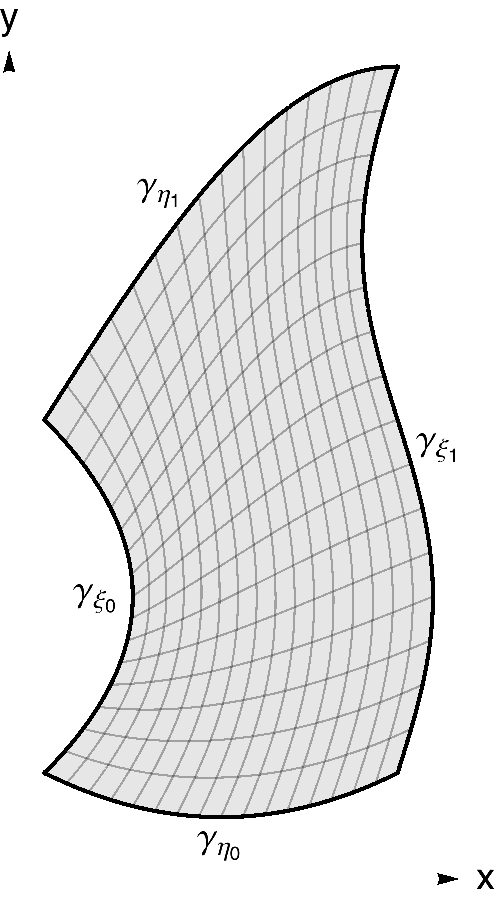
\includegraphics[width=.35\textwidth]{fig/testfig1.pdf}
\hspace{1cm}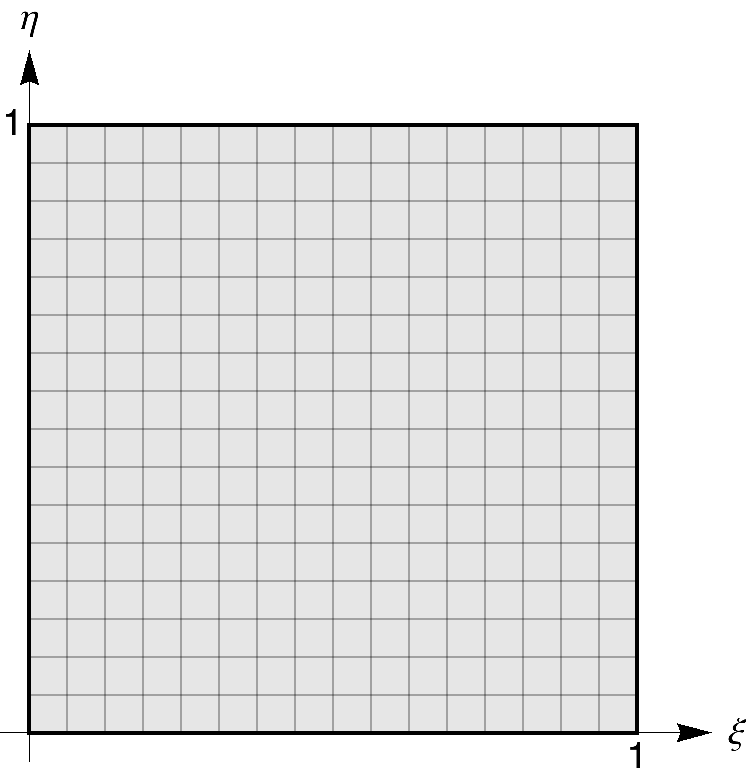
\includegraphics[width=.45\textwidth]{fig/testfig2.pdf}}
\caption{Figure Captions.}
\label{fig:label}
\end{figure}

\end{section}

\chapter{The Standard Model}
\begin{section}{Overview and Successes}

The Standard Model (SM) of particle physics is a wildly successfull theory and one of the greatest accomplishments in science.
Formulated in the second half of the 20th century, it describes 17 experimentally-observed, fundamental particles and their interactions through the electromagnetic, weak, and strong fundamental forces.
These particles, shown in Figure~\ref{fig:sm_particles}, consist of six quarks and six leptons, known as fermions, which comprise the matter particles, along with four gauge bosons and one scalar boson, which mediate particle interactions.

\begin{figure}[tbp!]
\begin{center}
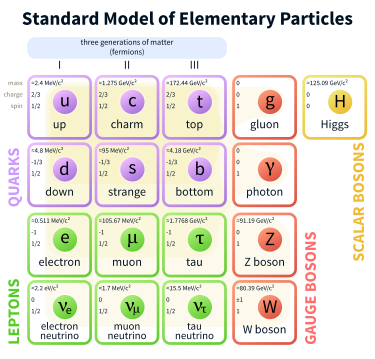
\includegraphics[angle=0,width=0.80\columnwidth]{fig/sm_particles.png}
\end{center}
\caption{The fundamental particles of the Standard Model and some of their properties.}
\label{fig:sm_particles}
\end{figure}

Formally, the Standard Model is quantum field theory with symmetries described by the group $\mrm{SU}_c(3) \times \mrm{SU}_L(2) \times \mrm{U}_Y(1)$ and with a Lagrangian of
\begin{align}
\mathcal{L} &= -\frac{1}{4}F_{\mu\nu}F^{\mu\nu} + i\overline{\psi}_i\slashed{D}\psi_i \nonumber \\
            &+ y_{ij}(\psi_{i}\psi_{j}+\bar{\psi}_{i}\bar{\psi}_{j})\phi + |D_{\mu}\phi|^2 - V(\phi),
\end{align}
where $F_{\mu\nu}$ is the field strength tensor, $D_{\mu}$ is the gauge covariant derivative, $\slashed{D} = \gamma^{\mu}D_{\mu}$, $\psi_{i}$ are the fermion fields, $\phi$ is the Higgs field, and $y_{ij}$ are the yukawa couplings.
In the top line, the first term of the Lagrangian describes the interactions of gauge bosons, while the second encodes the interactions between gauge bosons and fermions.
The bottom line describes Higgs physics with the first term describing the Higgs-fermion interactions, the second term encoding the Higgs-gauge boson interactions, and finally, the third term representing the Higgs potential.

As the Standard Model is able to provide predictions across an enormous scope of physics, it has been rigorously tested throughout its history.
For example, Figure~\ref{fig:sm_tests}, shows the agreement between the SM predictions and experimental results for the production cross section of a variety of processes.
Amazingly, all of the measurements, spanning nine order sof magnitude, agree with SM predictions.
At the same time, the Standard Model is the most precisely tested theory in physics with its prediction~\cite{PhysRevLett.109.111807} of the anamalous electron magnetic moment incredibly agreeing with experimental measurements~\cite{PhysRevLett.100.120801,PhysRevA.83.052122} at up to fourteen decimal places, as shown in Table~\ref{tab:ae_values}.

\begin{figure}[tbp!]
\begin{center}
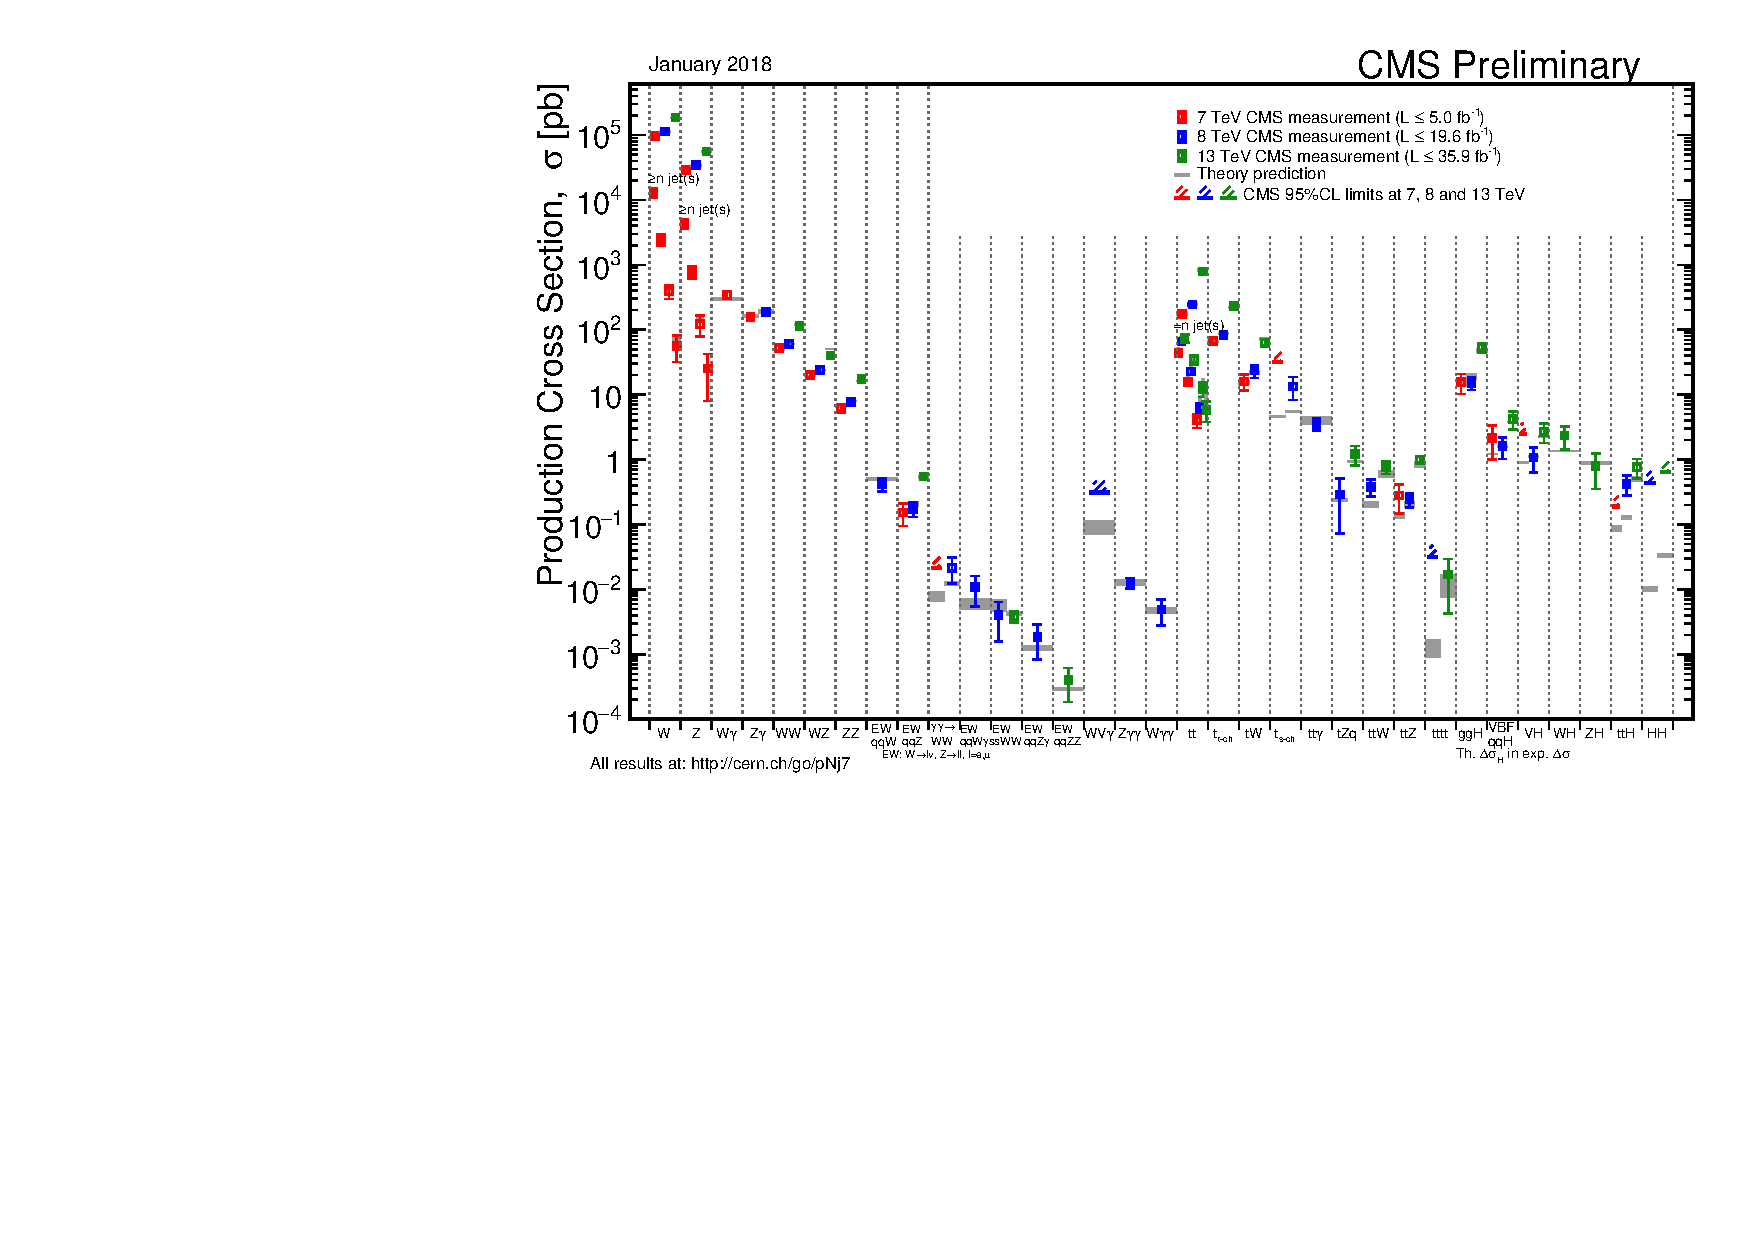
\includegraphics[angle=0,width=0.95\columnwidth]{fig/sm_tests.pdf}
\end{center}
\caption{The theoretical and experimental value for the production cross section of various processes~\cite{sm_tests}.}
\label{fig:sm_tests}
\end{figure}

\begin{table}[tbp!]
\centering
\begin{tabular}{ |c|c| }
\hline
$a_e \mrm{(Theory)}$      &  0.001 159 652 181 78(77) \\
$a_e \mrm{(Experiment)}$  &  0.001 159 652 180 73(28) \\
\hline
\end{tabular}
\caption{The theoretical~\cite{PhysRevLett.109.111807} and experimental~\cite{PhysRevLett.100.120801,PhysRevA.83.052122} values of the anamalous electron magnetic moment, $a_e$.
The uncertainty in the last digits is shown in parantheses.}
\label{tab:ae_values}
\end{table}

\end{section}

\begin{section}{The Standard Model as an Incomplete Theory}

Despite the impressive successes of the Standard Model, it is incomplete as a fundamental description of the unvierse and many tensions exist between it and both experimental and theoretical concerns.
For example, the Standard Model glaringly leaves out the fundamanetal force of gravity and attempts to construct a theory of quantum gravity have been frought with difficulties.
Furthermore, the Standard Model is unable to explain the substantial astrophysical evidence for dark matter~\cite{Bertone:2004pz,Rubin:1970zza}, which comprises $\sim 80\%$ of the matter in the universe, as it has no suitable candidate that can account for the observed mass density of dark matter.

Additionally, the Standard Model provides no mechanisms for:
\begin{itemize}
\item the origin of neutrino masses
\item the matter-antimatter symmetry
\item the presence of dark energy
\item a grand unified theory of the strong and electroweak forces
\end{itemize}

Because of these issues, the Standard Model is believed to be a low-energy effective field theory with new physics entering at higher energies.
It is, however, not easy to know what form this new physics may take, and thus solutions to the above problems have been used to drive much of the theoretical framework for extending the Standard Model.
In particular, the Hierarchy Problem and the idea of ``naturalness'', described in the section below, are, perhaps, the most significant lampposts in the search for new physics.

\begin{subsection}{The Hierarchy Problem and Naturalness}

The long-awaited discovery of the Higgs boson~\cite{Aad:2012tfa,Chatrchyan:2012xdj,Chatrchyan:2013lba,Khachatryan:2014jba,Aad:2014aba,Aad:2015zhl} confirmed the existence of a scalar boson with an observed mass of approximately $125~\GeV$.
This relatively low mass of the Higgs boson, however, creates two related theoretical concerns.
First, the Higgs mass is tied to the electroweak scale by the relation 
\begin{align}
v = \frac{\mh}{\sqrt{2}\lambda_h} \approx 246~\GeV,
\end{align}
where $v$ is the higgs vacuum expectation value (vev), \mh is the physical Higgs mass, and $\lambda_h$ is the Higgs Yukawa coupling.
The vev directly dictates the electroweak scale and is only on the order of 100~\GeV.
The next largest known energy scale is that of quantum gravity and is typically defined as the Planck mass, which is on the order of $10^{19}~\GeV$.
The question as to why these two scales are so discrepant is known as the Hierarchy Problem~\cite{Barbieri:1987fn}.

The second question stems from trying to understand the observed mass of the Higgs boson in the prescence of quantum corrections.
The Higgs mass can be broken down into two components, its bare mass, $m_{h,0}$, and contributions from radiative corrections, $\delta \mh^2$, as shown in the equation below
\begin{align}
\mh^2 = m_{h,0}^2 + \delta \mh^2.
\end{align}
As a scalar particle, the Higgs boson mass receives contributions from all massive particles, and in partcular, for a fermion, $f$, the contribution to the Higgs mass at the one-loop level, corresponding to the the diagram shown in Figure~\ref{fig:higgs_fermion_loop}, is of the form
\begin{align}
\delta \mh^2|_f &= -\frac{\lambda^2_f}{8\pi^2}N_f \int^{\Lambda_{UV}} \frac{d^4p}{p^2} \nonumber \\
                &= -N_f\frac{\lambda^2_f}{8\pi^2 } \left[\Lambda^2_{UV} - 6m_f^2\ln\left(\frac{\Lambda_{UV}}{m_f}\right) + 2m_f^2\right] + \mathcal{O}\left(\frac{1}{\Lambda^2}\right),
\label{eqn:higgs_fermion_correction}
\end{align}
with $\lambda_f$ the Yukawa coupling and $N_f$ the number of fermionic degrees of freedom.
The quantity $\Lambda_{UV}$ is the cutoff of the momentum integral, which represents the approximate scale at which the Standard Model is no longer valid.
In the case that there is no new physics beyond the Standard Model, this would correspond to $\Lambda_{UV} \sim \text{Planck scale} \sim 10^{19}~\GeV$, where effects due to quantum gravity are introduced.

\begin{figure}[tbp!]
\begin{center}
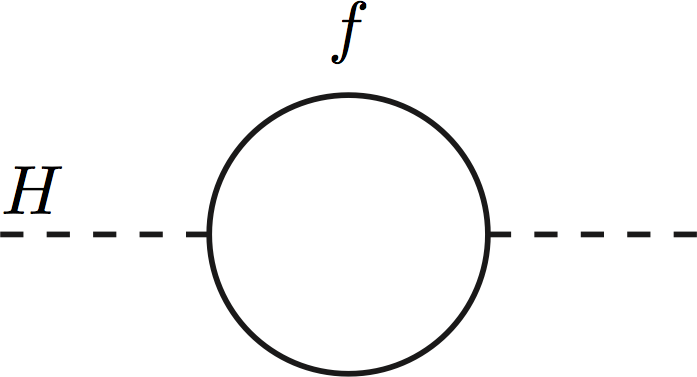
\includegraphics[angle=0,width=0.40\columnwidth]{fig/higgs_fermion_loop.png}
\end{center}
\caption{The fermionic one-loop Higgs mass correction.}
\label{fig:higgs_fermion_loop}
\end{figure}

In this scenario, the leading term of the Higgs mass corrections is $\mathcal{O}(10^{38}~\GeV^2)$, while, as measured, the squared Higgs mass is only $\mathcal{O}(10^{4}~\GeV^2)$.
For these two values to be consistent with each other, the Higgs bare mass parameter must exactly cancel the correction term at over 30 decimal places of precision.
This high-level of fine-tuning is considered to be ``unnatural'' and has been deemed the Naturalness Problem~\cite{Feng:2013pwa,Craig:2013cxa,Papucci:2011wy,Casas:2014eca}.
While it is entirely plausible that such a fine-tuned cancellation of parameters occurs -- there is no inherent theoretical reason against this, this problem motivates the need for new physics below the Planck scale, particularly physics that naturally incorporates a mechanism for cancelling the quadratic divergence of the $\Lambda_{UV}^2$ term.

\end{subsection}

\end{section}

\chapter{Supersymmetry}
\begin{section}{Natural Supersymmetry}

Supersymmetry (SUSY) is an extension of the Standard Model that introduces a new symmetry that relates fermionic and bosonic degrees of freedoms~\cite{ref:hierarchy1,ref:hierarchy2,Ramond:1971gb,Golfand:1971iw,Neveu:1971rx,Volkov:1972jx,Wess:1973kz,Wess:1974tw,Fayet:1974pd,Nilles:1983ge}.
This symmetry imposes that for every fermionic degree of freedom in the Standard Model, there exists a ``superpartner'' bosonic degree of freedom, and vice versa.
Furthermore, this symmetry dictates that both sets of particles couple to physics at the $\Lambda_{UV}$ scale identitically.

In the Minimal Supersymmetric Standard Model (MSSM)~\cite{Csaki:1996ks}, the Standard Model is extended to include a Higgs sector comprised of two scalar doublets and only the SM superpartners.
The superpartners of fermions are scalars and labeled by prefixing an ``s'' to the beginning of the corresponding SM particle name, while the superpartners of bosons are spin-1/2, labeled by suffixing an ``ino'' to the end of the corresponding SM particle name, and collecticely known as gauginos.
Thus, the SUSY particles consist of 4 higgsinos, 12 squarks, 9 sleptons, and 7 gauginos, where there are 2 scalar particles for each SM fermion in order to preserve the number of degrees of freedom.
The superpartners of SM particles are not necesarily mass eigenstates and can mix.
The gauge and mass eigenstates of the superpartners, along with their properties, are shown in Table~\ref{tab:susy_particles}.

\begin{table}[tb!]
\centering
\renewcommand{\arraystretch}{1.25}
\begin{tabular}{|c|c|c|c|c|}
\hline
Name                       &  Spin                &  Gauge Eigenstates                                            &  Mass Eigenstates \\
\hline
\hline  
Higgs bosons               &  0                   &  $H^0_u$ $H^0_d$ $H^+_d$ $H^-_d$                              &  $h^0$ $H^0$ $A^0$ $H^\pm$ \\
\hline
\multirow{3}{*}{squarks}   &  \multirow{3}{*}{0}  &  $\tilde{u}_L$ $\tilde{u}_R$ $\tilde{d}_L$ $\tilde{d}_R$      &  same \\
                           &                      &  $\tilde{c}_L$ $\tilde{c}_R$ $\tilde{s}_L$ $\tilde{s}_R$      &  same \\
                           &                      &  $\tilde{t}_L$ $\tilde{t}_R$ $\tilde{b}_L$ $\tilde{b}_R$      &  $\tilde{t}_1$ $\tilde{t}_2$ $\tilde{b}_1$ $\tilde{b}_2$\\
\hline
\multirow{3}{*}{sleptons}  &  \multirow{3}{*}{0}  &  $\tilde{e}_L$ $\tilde{e}_R$ $\tilde{\nu}_e$                  &  same \\
                           &                      &  $\tilde{\mu}_L$ $\tilde{\mu}_R$ $\tilde{\nu}_\mu$            &  same \\
                           &                      &  $\tilde{\tau}_L$ $\tilde{\tau}_R$ $\tilde{\nu}_\tau$         &  $\tilde{\tau}_1$ $\tilde{\tau}_2$ $\tilde{\nu}_\tau$\\
\hline
neutralinos                &  1/2                 &  $\tilde{B}^0$ $\tilde{W}^0$ $\tilde{H}^0_u$ $\tilde{H}^0_d$  &  $\tilde{N}_1$ $\tilde{N}_2$ $\tilde{N}_3$ $\tilde{N}_4$\\
\hline
charginos                  &  1/2                 & $\tilde{\Wboson}^\pm$ $\tilde{H}^+_u$ $\tilde{H}^-_d$         &  $\tilde{C}^\pm_1$ $\tilde{C}^\pm_2$ \\
\hline
gluino                     &  1/2                 & $\glu$                                                        &  same \\
\hline
\end{tabular}
\renewcommand{\arraystretch}{1}
\caption{The additional SUSY particles in the Minimal Supersymmetric Standard Model.}
\label{tab:susy_particles}
\end{table}

With the addition of these superpartners, a mechanism for naturally cancelling the radiative corrections to the Higgs mass is apparent, as the Higgs will couple to these new massive particles as well and provide additional radiative corrections that cancel the SM contributions.
For example, for a fermion $f$, the radiative corrections from the corresponding sfermion $\tilde{f}$, shown in Figure~\ref{fig:higgs_scalar_loop}, take the form
\begin{align}
\delta \mh^2|_{\tilde{f}} = &+N_{\tilde{f}}\frac{\lambda_{\tilde{f}}}{8\pi^2} \left[-\Lambda^2_{UV} + 2m_{\tilde{f}}^2\ln\left(\frac{\Lambda_{UV}}{m_{\tilde{f}}}\right)\right] \nonumber \\
                            &-N_{\tilde{f}}\frac{\lambda_{\tilde{f}}}{8\pi^2} \left[-2m_f^2 + 4m_f^2\ln\left(\frac{\Lambda_{UV}}{m_{\tilde{f}}}\right)\right] + \mathcal{O}(\frac{1}{\Lambda^2_{UV}})
\end{align}
using the relation $\sqrt{2}m_f = \lambda_f\nu$.
Supersymmetry imposes that $N_{\tilde{f}} = N_f$ and $\lambda_{\tilde{f}} = -\lambda_f^2$, and thus, in the case where $m_f = m_{\tilde{f}}$, this perfectly cancels not only the quadratic divergence in Equation~\ref{eqn:higgs_fermion_correction} but also the higher-order corrections, solving the Hierarchy and Naturalness Problems.

\begin{figure}[tbp!]
\begin{center}
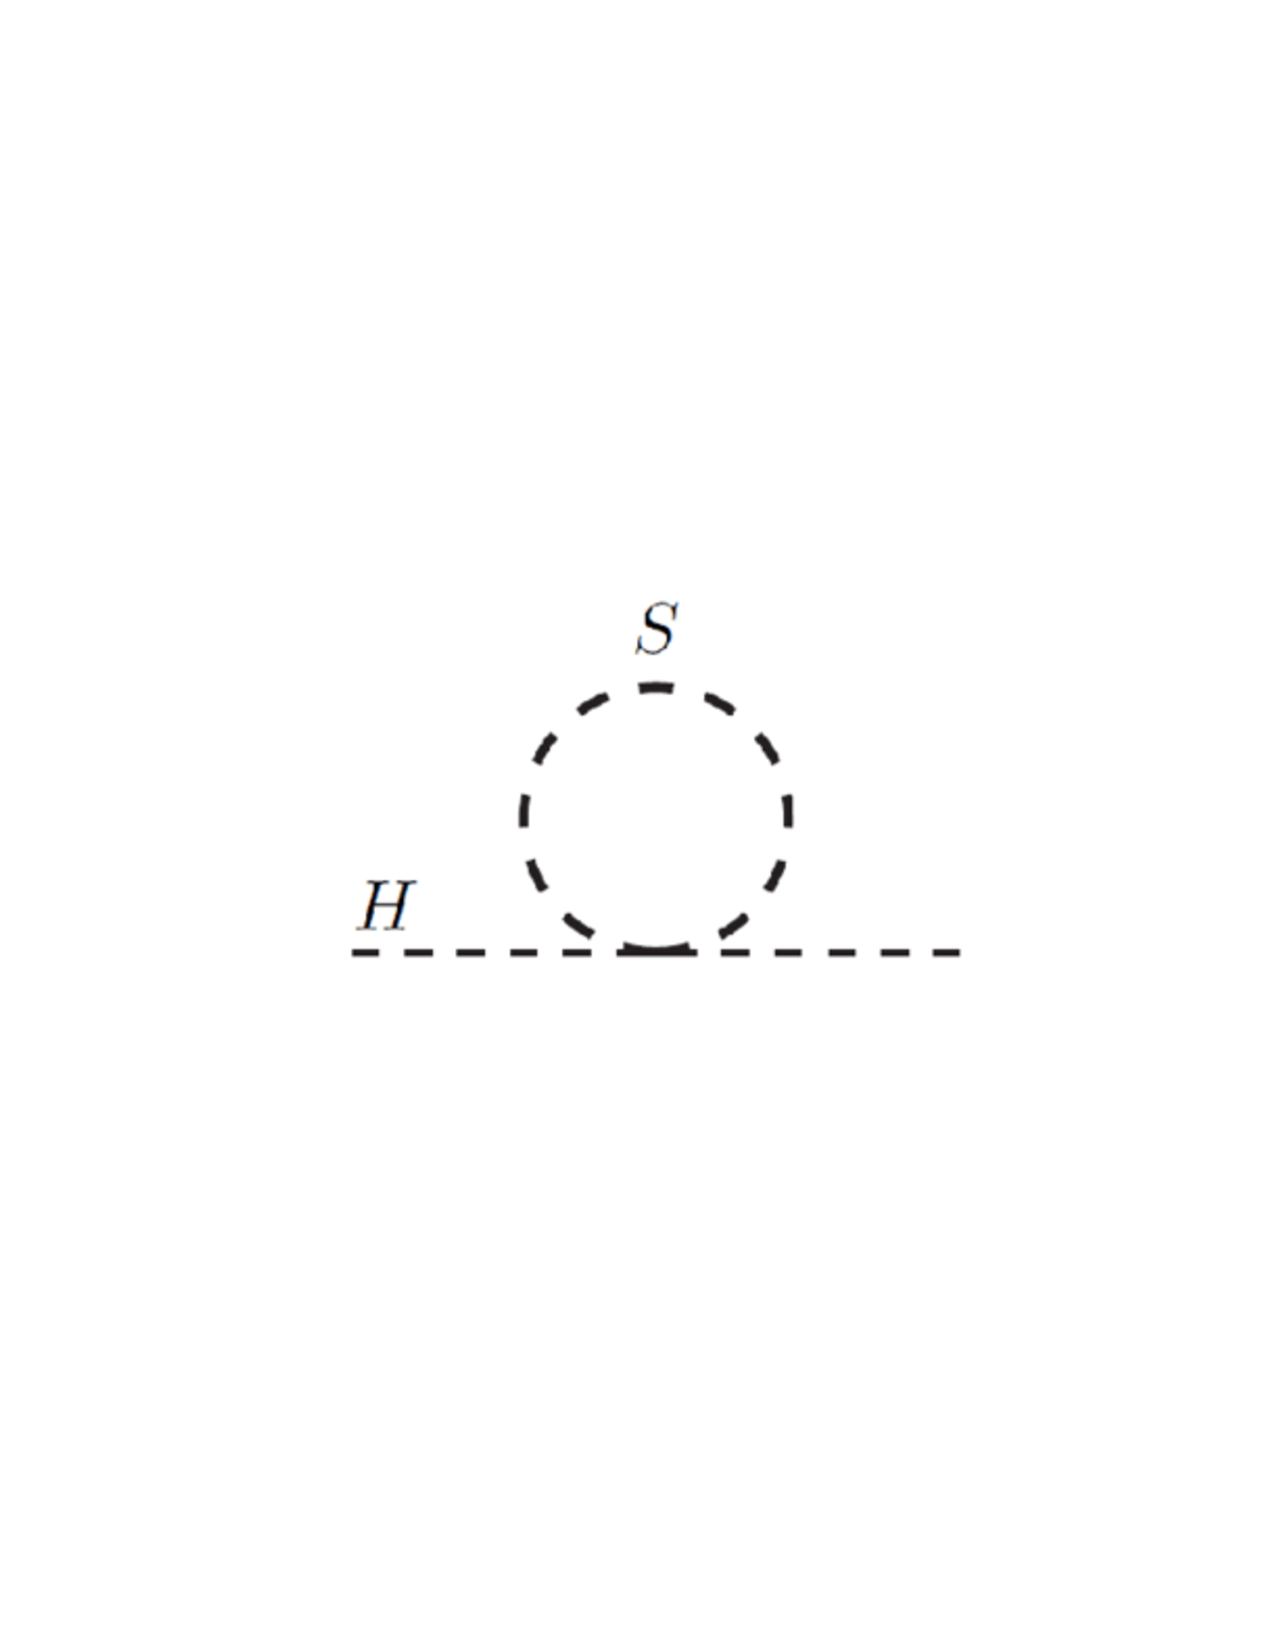
\includegraphics[angle=0,width=0.60\columnwidth]{fig/higgs_scalar_loop.pdf}
\end{center}
\caption{The scalar one-loop Higgs mass correction.}
\label{fig:higgs_scalar_loop}
\end{figure}

Of course, no superparticles have been observed at the SM scale.
This, however, does not imply that supersymmetry is incorrect but only that it may be a broken symmetry.
In this scenario where $m_f \neq m_{\tilde{f}}$, the quadratically divergent terms still cancel and what is left is only a lograithmic divergence, mediated by the squared mass difference of the partner particles:
\begin{align}
\delta \mh^2 = N_f\frac{\lambda_f^2}{8\pi^2} \left(m_f^2 - m_{\tilde{f}}^2\right) \ln\left(\frac{\Lambda_{UV}}{m_{\tilde{f}}}\right) + ...\ .
\label{eqn:total_higgs_correction}
\end{align}
This squared mass difference defines the degree to which the Higgs mass is fine-tuned.

\end{section}

\begin{section}{Phenemonological and Experimental Constraints}
\label{sec:susy_constraints}

While there is no theoretical prediction for the mass of the supersymmetric particles, there are certain guidelines for what the scale of these masses should be for a given level of fine-tuning that is deemed acceptable.
Firstly, the Higgsino masses are directly controlled by the value of $\mu$, which is related to the electroweak scale by
\begin{align}
-\frac{m_{\Zboson}}{2} = \mh^2 + |\mu|^2,
\end{align}
indicating that the Higgsino masses must be near the electroweak scale, $\sim 100~\GeV$, in order avoid a large fine-tuning of parameters.

The other superparticle masses are constrained by the size of their contributions to the Higgs mass, described in Equation~\ref{eqn:total_higgs_correction}.
Not all superparticles, however, contribute equally to the Higgs mass, and thus the phenemonological constraints for paritcles are in proportion to the size of their correction to the Higgs mass.
The largest constraint is on the stop squark masses due to the large Yukawa coupling of the top quark, which implies that the stop masses must be relatively light in order to keep the squared mass difference small and correspondingly the overall contribution small.
This also constrains the mass of the left-handed sbotom squark as it is in a doublet with $\tilde{t}_L$ and thus must not be much heavier.
Finally, the gluino couples to the squarks at the one-loop level, which means it still couples to the Higgs boson at the two-loop order, despite the Yukawa coupling for a gluon being zero.
This constraint on the gluino is looser than for other particles described, but since it is strongly interacting, it has a high cross section at the Large Hadron Collider (LHC) and is thus an important experimentally accessible particle.
Not considering model-dependent concerns, these are generically the only SUSY particles that are required to be light, and the rest of the superparticles may be decoupled with very high masses.
A qualitiative example of a natural SUSY spectrum is shown in Figure~\ref{fig:natural_susy_spectrum}.

\begin{figure}[tbp!]
\begin{center}
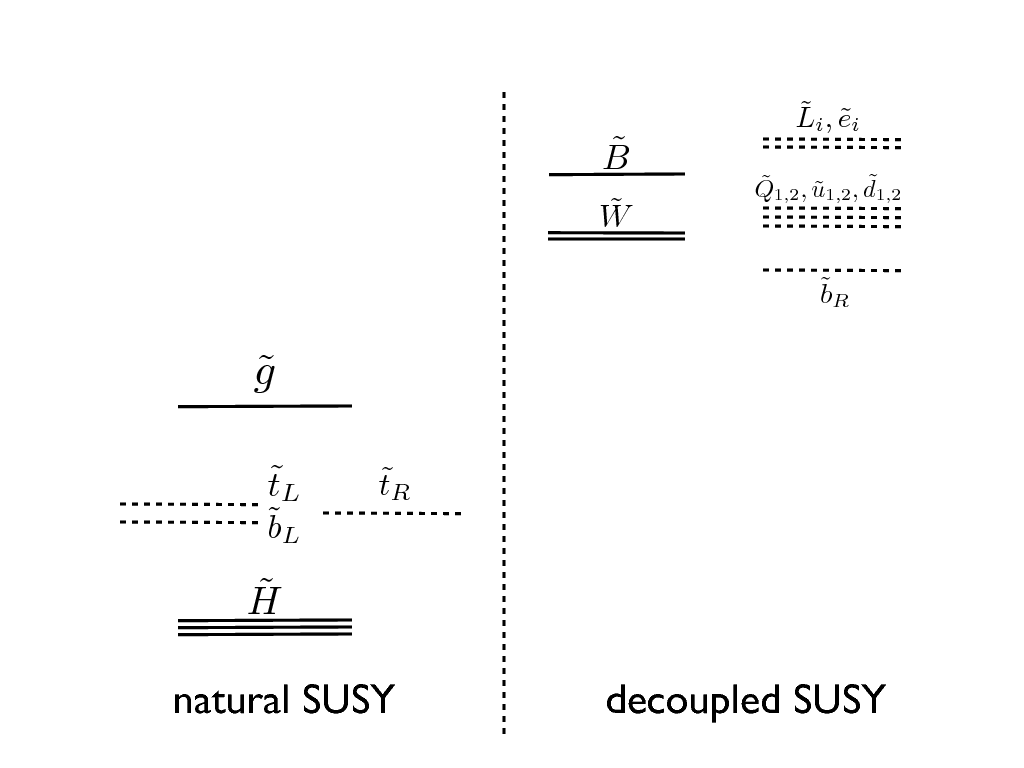
\includegraphics[angle=0,width=0.60\columnwidth]{fig/natural_susy_spectrum.png}
\end{center}
\caption{An example spectrum for natural SUSY~\cite{Papucci:2011wy}.}
\label{fig:natural_susy_spectrum}
\end{figure}

In order to gain a rough quantitative sense of what the mass constraints for these particles are, a measure of the Higgs mass fine-tuning can be constructed as
\begin{align}
\mathcal{N} \equiv \frac{\delta\mh^2}{\mh^2}.
\end{align}
Thus for $\mathcal{N} = 10$, a fine tuning of 1 part in 10, the bounds are $m_{\tilde{t}} \lesssim 1~\TeV$ and correspondingly $m_{\tilde{b}} \lesssim 1~\TeV$ and $\mglu \lesssim 2~\TeV$.

Recent results from the LHC, however, are already starting to threaten these bounds, as shown in Figure~\ref{fig:cms_susy_results} and Figure~\ref{fig:atlas_susy_results}, with gluino and stop exclusion limits already surpassing these bounds for certain models.
These constraints, however, are largely in the context of \RPC models, where a new quantum number, $P_R$, is conserved.
\RP is defined per particle as
\begin{align}
P_R \equiv (-1)^{3(B-L)+2s},
\end{align}
where $B$, $L$, and $s$ is the baryon number, lepton number, and spin of the particle.
This results in $P_R = +1$ for SM particles and $P_R = -1$ for SUSY particles.
The motivation for requiring that \RP be conserved is that the lightest supersymmetric particle (LSP), in this case, cannot decay to SM particles and is therefore stable.
For models where the LSP is a neutralino, the LSP is then a dark matter candidate.

\begin{figure}[tbp!]
\begin{center}
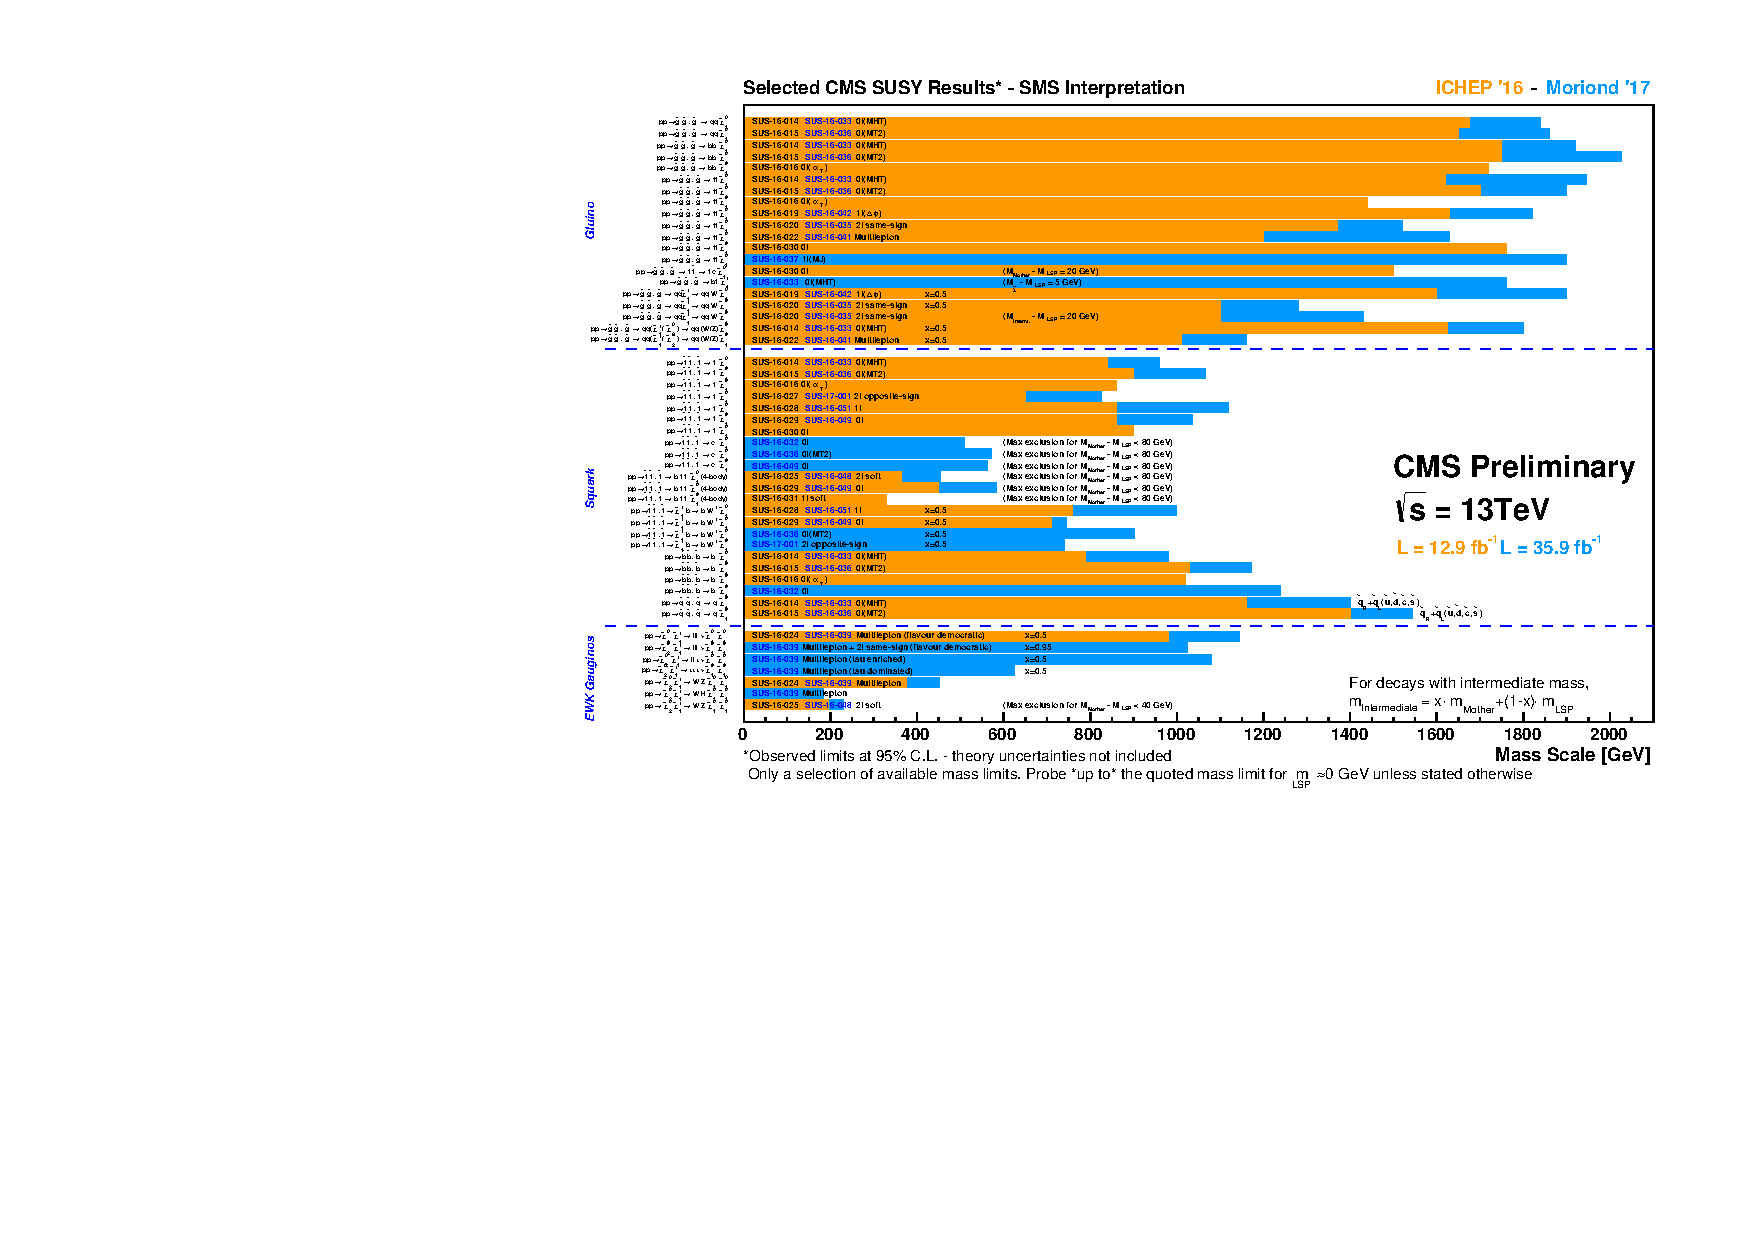
\includegraphics[angle=0,width=0.95\columnwidth]{fig/cms_susy_results.pdf}
\end{center}
\caption{An overview of recent results from SUSY searches from the Compact Muon Solenoid experiment~\cite{cms_susy_results}.}
\label{fig:cms_susy_results}
\end{figure}

\begin{figure}[tbp!]
\begin{center}
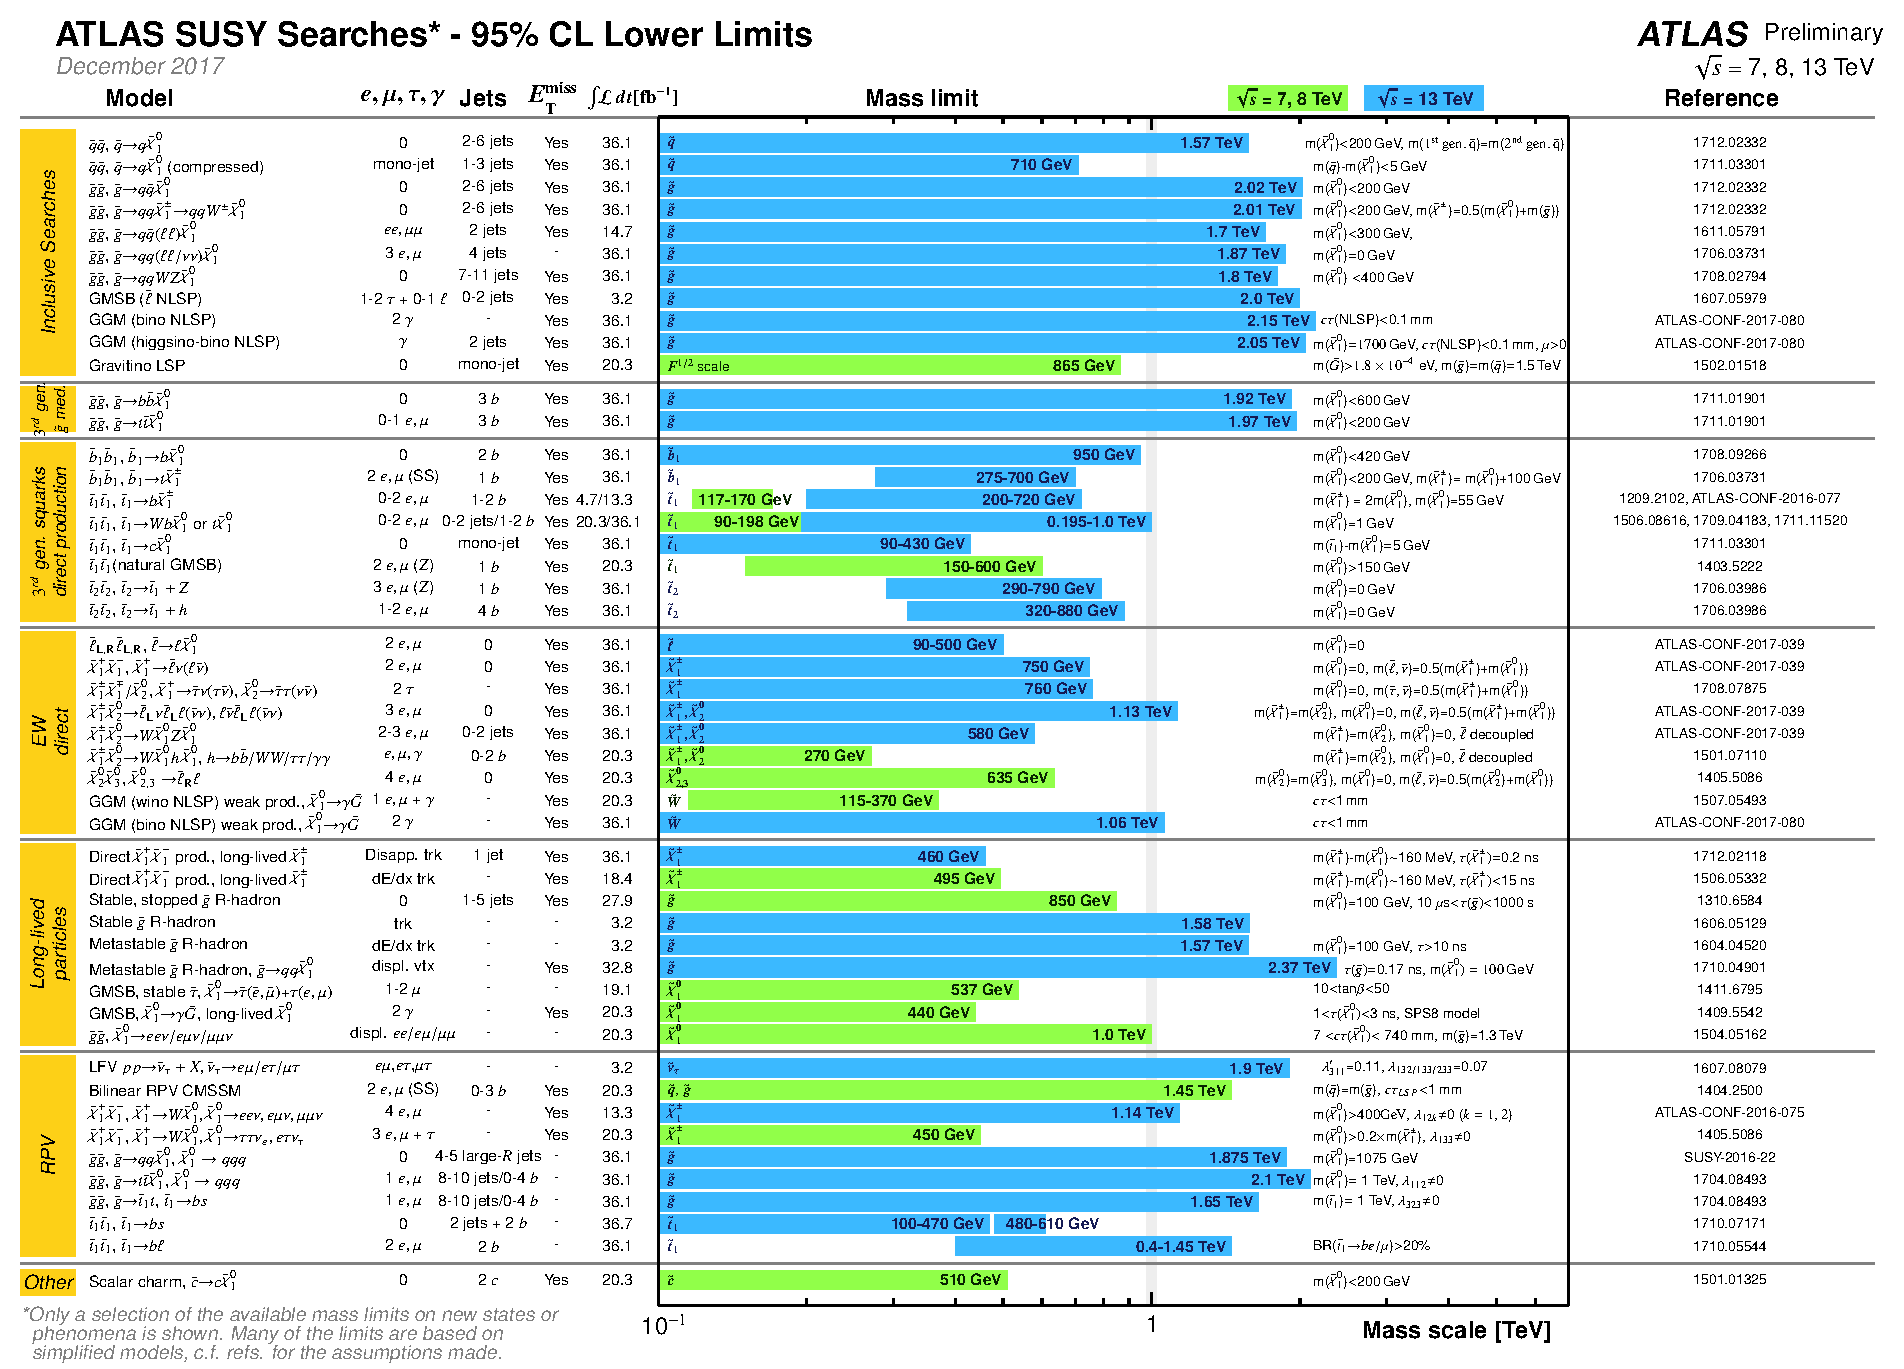
\includegraphics[angle=0,width=0.90\columnwidth]{fig/atlas_susy_results.pdf}
\end{center}
\caption{An overview of recent results from SUSY searches from the A Toroidal LHC Apparatus experiment~\cite{atlas_susy_results}.}
\label{fig:atlas_susy_results}
\end{figure}

The phenomenology, however, for \RPC (RPC) and \RPV (RPV) SUSY models is very different.
For RPC scenarios, the stable LSP does not interact with the detector and escapes without depositing any energy.
The presence of the LSPs, however, can be inferred by examining the missing transverse momentum (\MET) in an event, which due to the negligible transverse momentum of the initial colliding particles, should be 0 in events without LSPs or neutrinos.
Thus, the \MET in an event provides a powerful handle for discriminating signal and background and most analyses search for signatures that include significant amounts of \MET.
In RPV models, however, the LSP is not stable and decays to SM particles, which does not produce a large \MET signature.
Although this disfavor the LSP as a dark matter candidate, it allows RPV models to evade the constraints from RPC searches.
Subsequently, RPV SUSY yields an important class of models that can ease the tension between natural solutions to the hierarchy problem and current experimental limits.

\end{section}

\begin{section}{\RP Violating Supersymmetry}

In the MSSM, the additional \RPV terms are
\begin{align}
W_{RPV} = \frac{1}{2}\lambda^{ijk}L_{i}L_{j}\overline{\mrm{e}}_{k} + \lambda^{'ijk}L_{i}Q_{j}\overline{\mrm{d}}_{k} + \frac{1}{2}\lambda^{''ijk}\overline{\mrm{u}}_{i}\overline{\mrm{d}}_{j}\overline{\mrm{d}}_{k} + \mu^{'i}L_{i}H_{u},
\end{align}
where the color indices have been surpressed and the letters $i$, $j$, $k$ denote generation.
The fields $L_{i}$, $Q_{j}$, and $H_u$ are SU(2) doublets corresponding to leptons, quarks, and the Higgs boson, respectively, while $\overline{\mrm{e}}_k$, $u_i$, and $d_j$ are the charged lepton, up-type quark, and down-type quark SU(2) singlets.
The $\mu$ and various $\lambda$ factors are coupling strengths for their corresponding interactions, where $\lambda$ and $\lambda^{''}$ must be antisymmetric in their first and last two indices, respectively, due to color conservation.
A full description of RPV SUSY can be found in Reference~\cite{Barbier:2004ez}.

While there is no fundamental theoretical reason forbidding \RP violation, there are significant constraints on these interactions, primarilly due to the lepton number violating (LNV) couplings, $\lambda$ and $\lambda^{'}$, and and the baryon number violating (BNV) coupling, $\lambda^{''}$~\cite{Allanach:1999ic}.
The most stringent of these constraints is from proton decay on which current experimental results place a lower bound on the proton half-life of $\mathcal{O}(10^{34}\ \mrm{years})$~\cite{Bajc:2016qcc,Nishino:2009aa}.
Proton decay, however, requires both a lepton number and baryon number violating coupling, as shown in Figure~\ref{fig:proton_decay}.
This constraint can be avoided if a mechanism exists to make one of these couplings zero or negligibly small.
Additionally, though, there are strong limits on the individual LNV and BNV couplings, for example from neutron oscillation and muon-to-electron decay measurements, which are most stringent for the light generations.
Thus, for any mechanism to evade these constraints, it must also motivate smaller couplings for the lighter generations.

\begin{figure}[tbp!]
\begin{center}
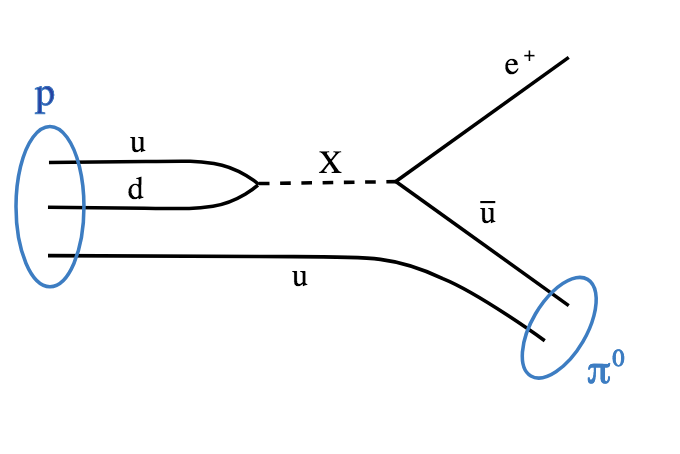
\includegraphics[angle=0,width=0.60\columnwidth]{fig/proton_decay.png}
\end{center}
\caption{Example diagram representing proton decay, where the particle X represents a down-type squark~\cite{Allanach:2016yth}.
The left vertex is mediated by the baryon number violating coupling, $\lambda^{''}$, and the right vertex is mediated by the lepton number violating coupling, $\lambda^{'}$.}
\label{fig:proton_decay}
\end{figure}

\begin{subsection}{Miminal Flavor Violating Supersymmetry}

One way to avoid the constraints placed on the RPV couplings is to construct a model by following the structure of minimal flavor violation.
In these Minimal Flavor Volating (MFV) SUSY models~\cite{Csaki:2013we,Krnjaic:2012aj,Csaki:2011ge}, the RPV couplings are related to the SM Yukawa couplings, making the third generation RPV couplings large and those of the first two small.
For example, the $\lambda^{''}$ coupling can be written as
\begin{align}
\lambda^{''}_{ijk} = w^{''} y^{(u)}_i y^{(d)}_j y^{(d)}_k \epsilon_{jkl} V^{*}_{il}
\end{align}
with $w^{''}$ an $\mathcal{O}(1)$ parameter, $y^{(u)}$ and $y^{(d)}$ the up- and down-type Yukawa couplings, and $V$ the CKM matrix.
From this, the sizes of the $\lambda^{''}_{ijk}$ couplings can be roughly estimated (using $w^{''} = 1$) and are shown in Table~\ref{tab:mfv_couplings}, which depicts the dependence of the coupling strength on generation.
Additionally, in MFV scenarios, the LNV couplings are severly suppressed by neutrino masses, and in the limit of massless neutrinos, are exactly zero.
Thus, the only relevant RPV coupling in MFV SUSY models is the BNV $\mkern1mu\overline{\mkern-1mu\mrm{u}\mkern-1mu}\mkern1mu\mkern1mu\overline{\mkern-1mu\mrm{d}\mkern-1mu}\mkern1mu\mkern1mu\overline{\mkern-1mu\mrm{d}\mkern-1mu}\mkern1mu$ coupling, which is small for the first two generations -- meeting the exact criteria necessary to evade experimental constraints on RPV couplings.
Furthermore, in the case where the LSP is a squark, it will decay promptly and not produce \MET, allowing these models to even evade the constraints from RPC SUSY searches.

\begin{table}[tbp!]
\centering
\begin{tabular}{ |c|ccc| }
\hline
     &  $ds$                 &  $db$                &  $bs$               \\
\hline
$u$  &  $3 \times 10^{-12}$  &  $6 \times 10^{-9}$  &  $5 \times 10^{-7}$ \\
$c$  &  $1 \times 10^{-8}$   &  $1 \times 10^{-5}$  &  $4 \times 10^{-5}$ \\
$t$  &  $4 \times 10^{-5}$   &  $6 \times 10^{-5}$  &  $2 \times 10^{-4}$ \\
\hline
\end{tabular}
\caption{Rough estimates for the sizes of the $\lambda^{''}_{ijk}$ MFV RPV couplings~\cite{Csaki:2011ge}.}
\label{tab:mfv_couplings}
\end{table}

Because of these considerations, MFV SUSY is an intriguing class of models to investigate experimentally.
In particular, due to the high $\glu\glu$ cross-section and large value of $\lambda^{''}_{\mrm{t}\mrm{b}\mrm{s}}$, a search for the pair-production of gluinos that decay via \rpvDecay, as shown in Figure~\ref{fig:rpv_decay}, is well-motivated.

The remainder of this dissertation is dedicated to describing such a search conducted with the Compact Muon Solenoid detector using $\sqrt{s} = 13~\TeV$ proton-proton collisions.

\begin{figure}[tbp!]
\begin{center}
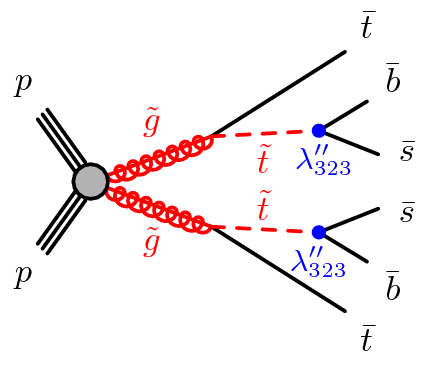
\includegraphics[angle=0,width=0.40\columnwidth]{fig/rpv_decay.png}
\end{center}
\caption{Example diagram of the pair production of gluinos that decay via \rpvDecay.}
\label{fig:rpv_decay}
\end{figure}

\end{subsection}

\end{section}

\part{Experimental Apparatus}
\chapter{Experimental Apparatus}

While the Large Hadron Collider was approved over 20 years ago, much of its design was influenced by the needs of searches for physics beyond the Standard Model (BSM).
The two most important properties of a collider, for a BSM search, are its center-of-mass energy and its (instantaneous) luminosity, both of which were designed to be higher than any previous experiment. 
The designed center-of-mass energy ($\sqrt{s}$) of $14~\TeV$ allows for the production of particles heavier than ever previously, while the designed luminosity of $10^{34}~\cm^{-2}\s^{-1}$ allows BSM searches to probe very rare processes.

In the same way, the design of the Compact Muon Solenoid (CMS) detector reflects the needs of BSM searches.
In particular, to fully search the uncovered parameter space of new physics an all-purpose, hermitic detector that can precisely measure a variety of particles and reliably determine the MET in an event is needed to cover the many (un)theorized new physics models.

This chapter summarizes in more detail the major features of both the LHC and CMS.
A complete description of both can be found in Refs.[INCLUDE].

\begin{section}{The Large Hadron Collider}

The LHC since 2015 has been colliding protons together at $\sqrt{s} = 13~\TeV$, slightly below the designed specifications but still at an unsurpassed energy.
In order to reach this center-of-mass energy, the LHC uses a large accelerator complex consisting of a sucession of many smaller particle accelerators, which is necessary to produce protons and bring them up to a speed such that they can be injected into the LHC ring.
A diagram of the CERN accelerator complex is shown in Figure~\ref{fig:lhc_accelerator_complex}.

\begin{figure}[tbp!]
\begin{center}
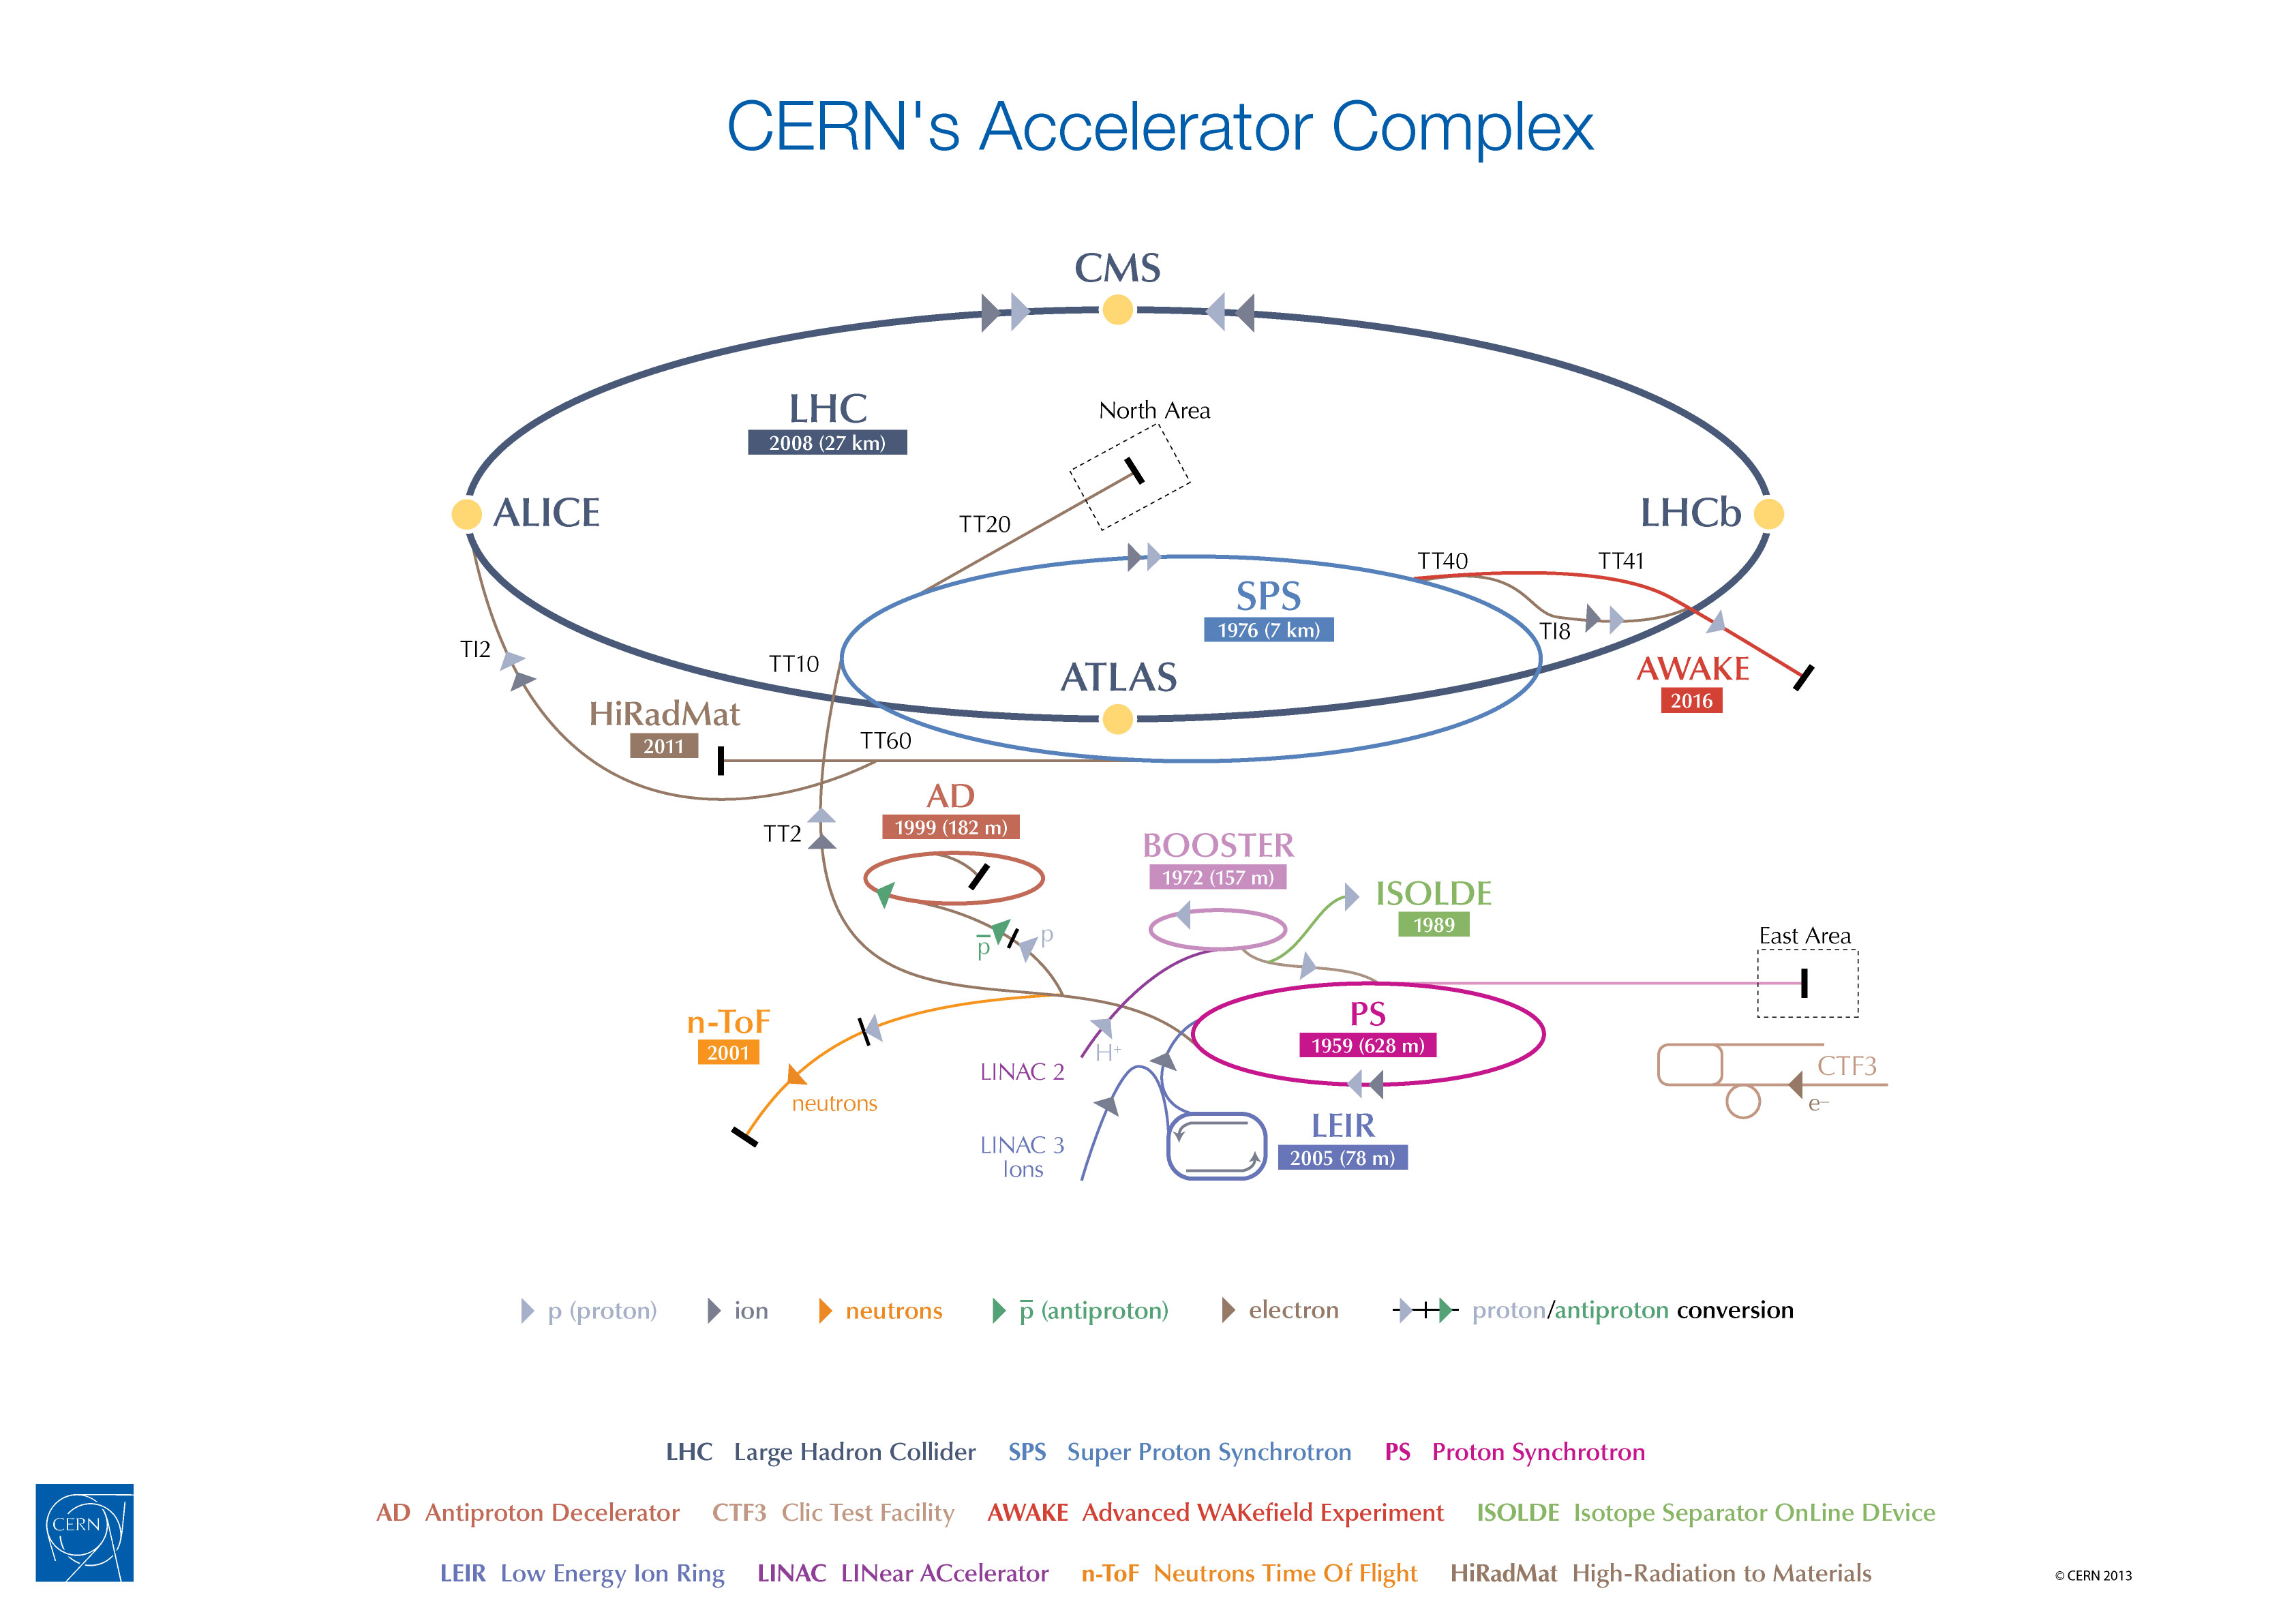
\includegraphics[angle=0,width=0.95\columnwidth]{fig/lhc_accelerator_complex.jpg}
\end{center}
\caption{A schematic of the CERN LHC accelerator complex.~\cite{Marcastel:1621583}}
\label{fig:lhc_accelerator_complex}
\end{figure}

This process first begins with a simple bottle of hydrogen gas, which are ionized by an electric field to produce the needed protons.
These resulting protons are then fed into LINAC 2, the first accelerator in the chain, which accelerates them up to $50~\MeV$, creating a beam of protons.
The proton beam is then passed succesively to the Proton Synchtron Booster, Proton Synchotron, and Super Proton Synchtron, where the beam reaches energies of $1.4~\GeV$, $25~\GeV$ and $450~\GeV$, respectively.
At the Proton Synchotron, the beams are additionally split into ``bunches'', each consisting of $O(10^{11})$ protons and separated in time by 25~ns. 
Finally, the protons can be injected into the two beam pipes of the LHC, each circulating in opposite directions. 
These beams continue to be accelerated until they reach their final energy of $6.5~\TeV$, allowing for collisions at $\sqrt{s} = 13~\TeV$.
At this point, the proton beams are focused and fine-tuned at several stages in order to increase the luminosity. 
In 2016, the LHC was able to collide protons with an instantaneous luminosity of $1.4~\times~10^{34}~\cm^{-2}\s^{-1}$, exceeding its designed specification, and deliver a record-high integrated luminosity of $41.07~\ifb$.

These improvements from previous generations of colliders greatly increase the reach of searches for new, heavy particles.
Since the center-of-mass energy of the actual colliding partons ($\sqrt{\hat{s}}$) is typically much less than the overall center-of-mass energy, raising the collider's energy can greatly increase the production cross-section of heavy particles, especially of those around the \TeV scale. 
For example, Figure~\ref{fig:parton_lumi}, which depicts the ratio of parton luminosities at $\sqrt{s} = 13~\TeV$ and $8~\TeV$ as a function of the characteristic mass scale of the event, shows that a $2000~\GeV$ gluino will be produced through $gg$ scattering processes ${\sim}15\times$ more often with less than a doubling of the collider energy.
Increasing a collider's energy, however, is not always a practical option, involving new technologies, expensive upgrades, or even a new collider. When this is the case, the best alternative to continue to probe rare processes is to simply take more data, more quickly, which a high luminosity collider like the LHC allows for.


\begin{figure}[tbp!]
\begin{center}
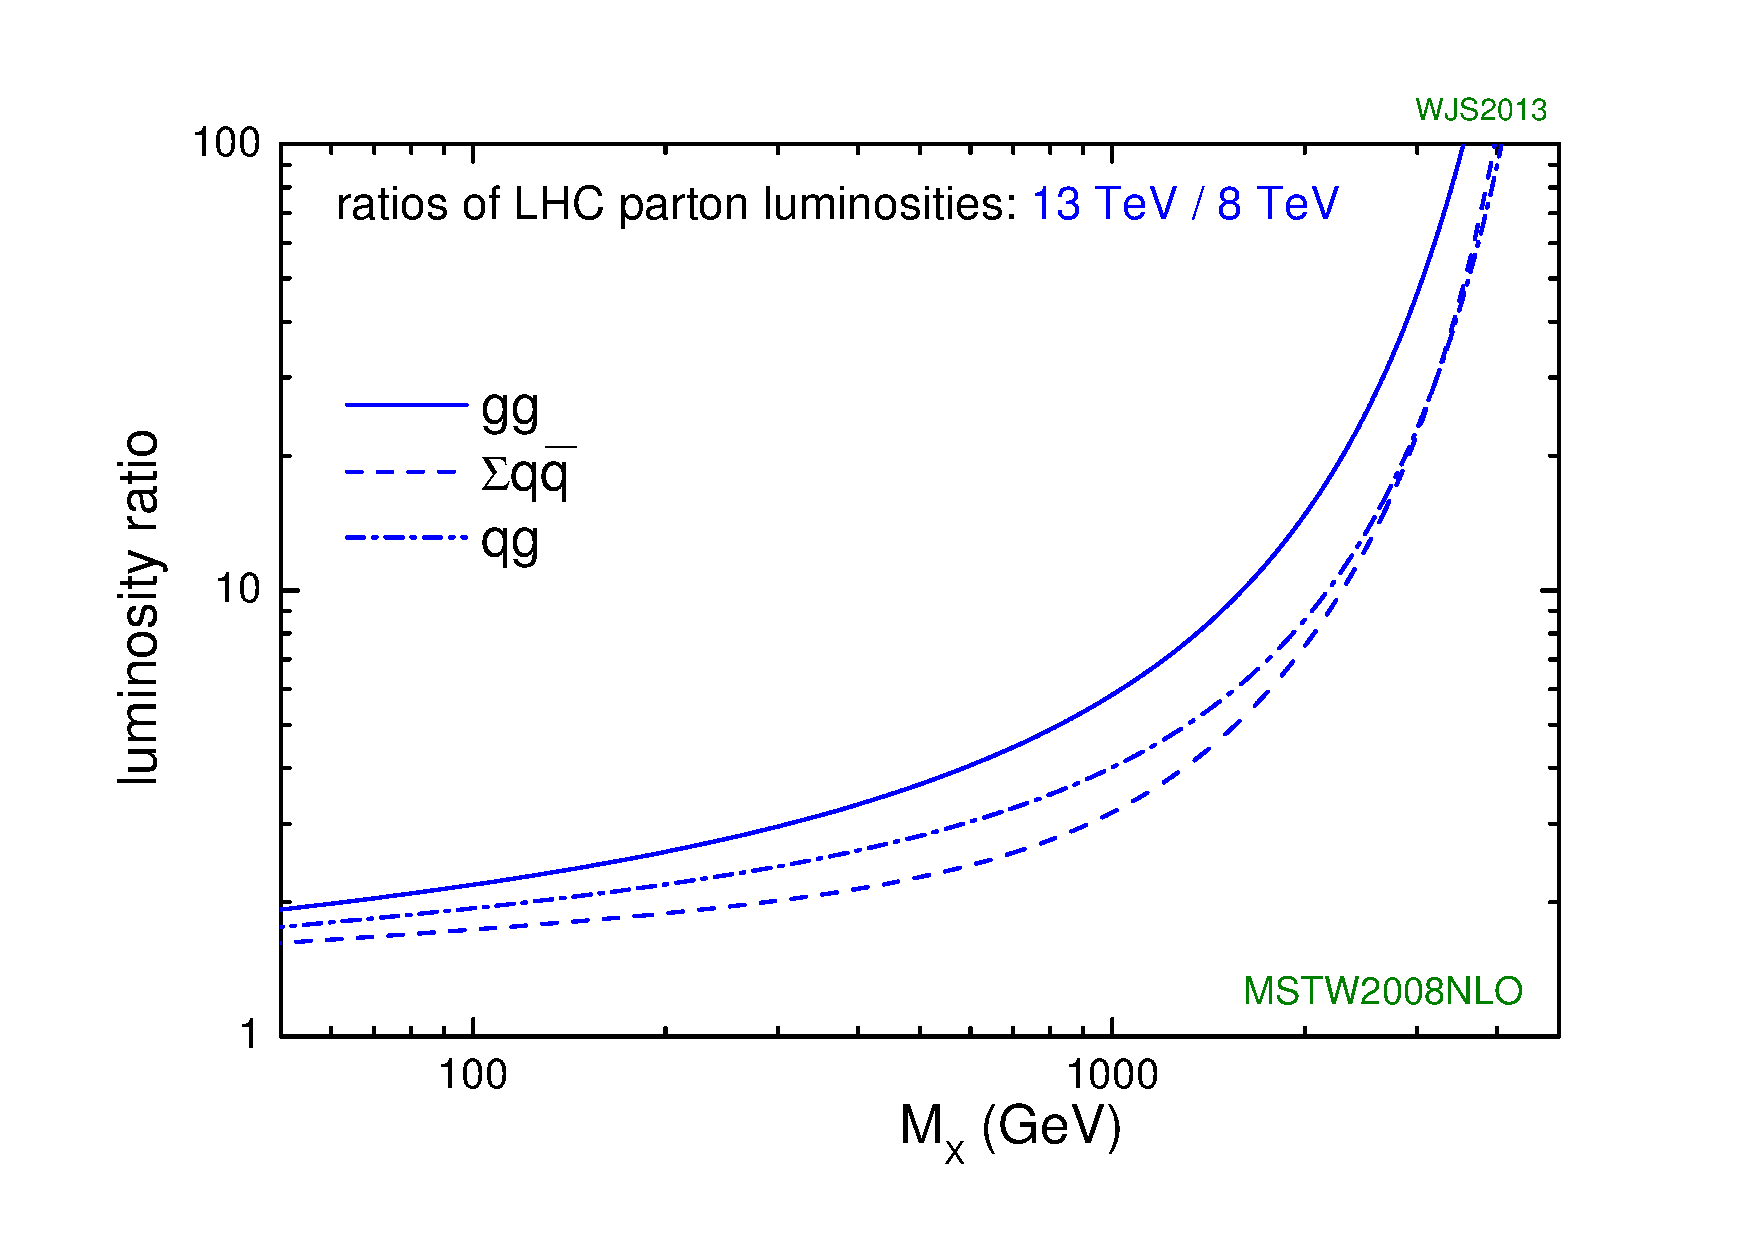
\includegraphics[angle=0,width=0.80\columnwidth]{fig/parton_lumi.pdf}
\end{center}
\caption{Ratio of parton luminosities at $\sqrt{s} = 13$ and $8~\TeV$.~\cite{parton_lumi}}
\label{fig:parton_lumi}
\end{figure}


\end{section}

\begin{section}{Compact Muon Solenoid}

Along the tunnels of the LHC, below Cessy, France, sits the CMS detector where the proton-proton collisions are recorded.
The overall shape of the detector is cylindrical with a length of $21.6~\m$ and radius of $7.3~\m$, while weighing roughly 14,000 metric tons.  
The CMS detector is sometimes called a cylindrical onion, as this shape is constructed through layers of specialized detectors, each designed to provide precise measurements for a particular particle type.
Peeling back the layers from the outside-in, the first sub-detector is the muon system. 
Next is a superconducting solenoid of $6~\m$ internal diameter that produces a magnetic field of $3.8~\mrm{T}$, and perhaps most importantly provides the ``S'' in CMS.
Placed within the solenoidal magnet, is the rest of the CMS detector, namely the Hadronical Calorimeter (HCAL), Electromagnetic Calorimeter (ECAL), and a silicon tracker.
The design of fitting most of the detector components within the solenoid is responsible for the ``C'' in CMS.
A diagram of the layout of the CMS detector can be seen in Figure~\ref{fig:cms_detector}.

\begin{figure}[tbp!]
\begin{center}
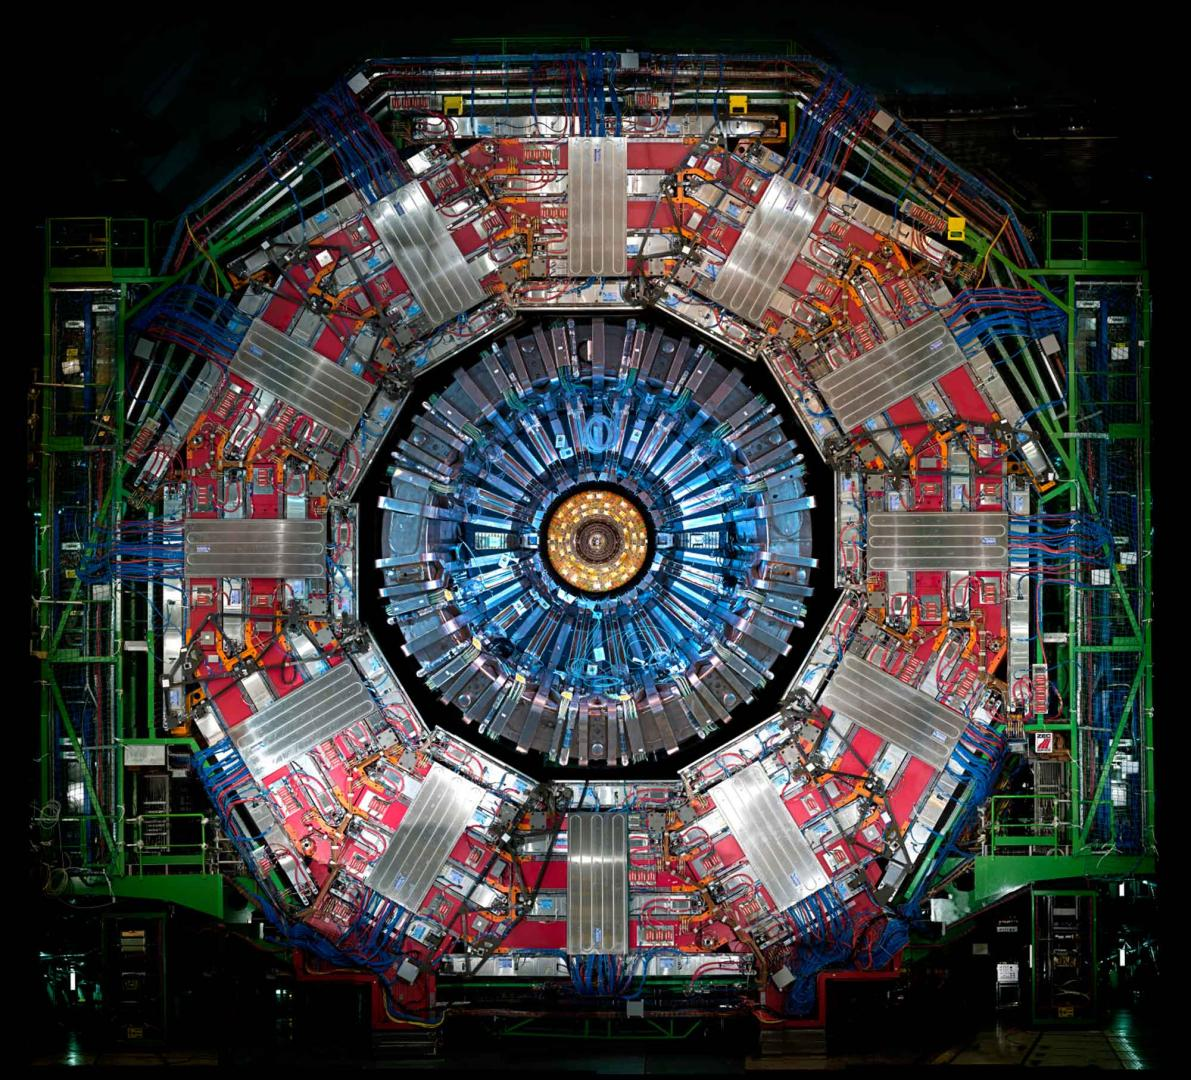
\includegraphics[angle=0,width=0.80\columnwidth]{fig/cms_detector.jpg}
\end{center}
\caption{A diagram showing the various sub-detectors of the CMS detector.~\cite{10.1088/978-1-6817-4078-2ch4}}
\label{fig:cms_detector}
\end{figure}

At the center of the silicon tracker is Interaction Point 5, the beam crossing which provides the proton-proton collisions to the CMS detector, and is the nominal origin of CMS's coordinate system.
The $x$-axis is defined to point towards the center of the LHC ring and the $y$-axis is defined to point up towards the surface, both of which are transverse to the proton beam. 
The $z$-axis points along the beamline with the positive direction given by the right-hand rule relative to the $x$- and $y$-axes.
Due to CMS detector shape, it is often useful to convert the cartesian coordinates to a cylindrical coordinate system.
In this system, the azimuthal angle, $\phi$, is measured from the $x$-axis in the $xy$-plane, and the polar angle, $\theta$, is measured from the z-axis.
The polar angle, however, is often replaced by psuedorapidity, defined as $\eta = -\ln(\theta/2)$.
Thus, any point in the CMS coordinate system can be represented by $(z, \eta, \phi)$.
A diagram showing both the cartesian and cylindrical coordinate systems can be seen in Figure~\ref{fig:cms_coordinate_system}.

The remainder of this section briefly describes the meain features of the various CMS sub-detectors.

\begin{figure}[tbp!]
\begin{center}
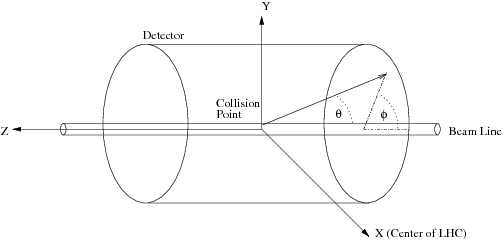
\includegraphics[angle=0,width=0.80\columnwidth]{fig/cms_coordinate_system.png}
\end{center}
\caption{A diagram of the cartesian and cylindrical coordinate systems used by CMS.~\cite{Schott:1699952}}
\label{fig:cms_coordinate_system}
\end{figure}

\begin{subsection}{Inner Tracking System}

The tracking system is used for precise measurements of the trajectories of charged particles, as well as reconstruction of seconday vertices.
As the tracking system is the closest subdetector to the interaction point, it faces a very large particle flux rate and so must be able to provide both high granularity and fast response, as well be able to survive operating in those conditions with ane expected lifetime of 10 years.
At the same time, these features must be balanced with minimizing the amount of material in order to reduce unwanted interactions with the detector, such as multiple scattering, photon conversion, and nuclear interactions.
These requirements lead to a tracking system composed entirely of silicon technology.

The CMS tracking system is actually composed of two parts.
The first is the pixel detector, which surrounds the interaction point, and is composed of 3 barrel layers at radii between $4.4$ and $10.2~\cm$ and 2 endcap layers that extend the acceptance up to $|\eta|<2.5$.
In total, the pixel detector covers an area of roughly $1~\m^2$ with 66 million pixels and achieves a resolution of roughly 10 and 20 microns in the directions transverse and logitudinal to the beam line, respectively.

The second part of the tracking system is the strips detector which sits just outside the pixel detector.
The strips detector is composed of 4 parts: the tracker inner barrel (TIB), tracker inner disks (TID), tracker outer barrel (TOB), and the tracker endcaps (TEC).
The TIB and TID extend up to $55~\cm$ in radius and are composed of 4 and 3 layers, respectively, while the TOB, which surronds the TIB and TID, extends out to $116~\cm$ and is composed of 6 layers.
Lastly, the TEC which sits next to the other strip detector components, covers a radius of 22.5 to $113.5~\cm$ and is composed of 9 disks.
In total, the strips detector covers an area of $198~\m^2$ with 9.3 million strips.
A layout of the tracking system including the pixel and strips detector is shown in Figure~\ref{fig:cms_tracker}.

\begin{figure}[tbp!]
\begin{center}
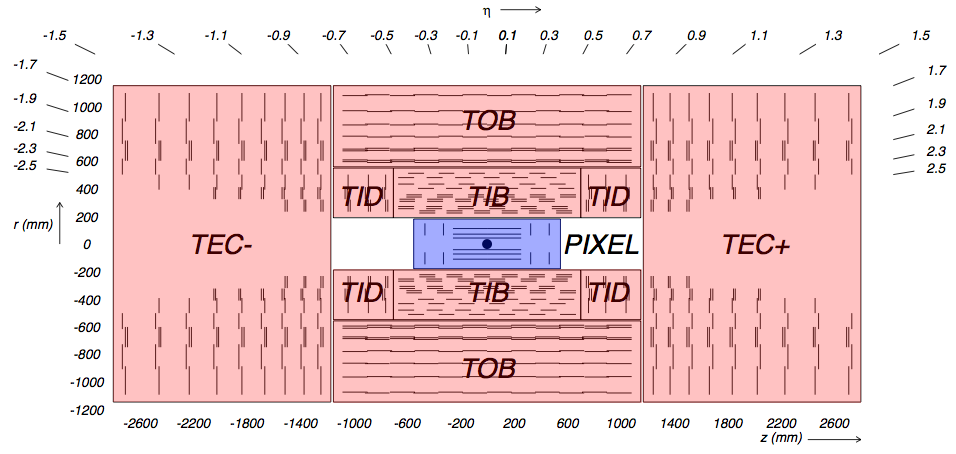
\includegraphics[angle=0,width=0.80\columnwidth]{fig/cms_tracker.png}
\end{center}
\caption{Layout of the CMS tracking system, showing both the pixel detector (blue) and the strips detector (red).~\cite{Lenzi:2013xpa}}
\label{fig:cms_tracker}
\end{figure}

\end{subsection}

\begin{subsection}{Electromagnetic Calorimeter}

The primary purpose of the electromagnetic calorimeter (ECAL) is to measure the energy of electrons and photons.
The ECAL is a hermetic, hemogenous detector made up of a barrel part, convering the $|\eta|<1.479$ region, and two endcap parts that covers $1.566<|\eta|<3.0$.
Both the barrel and endcap sections are comprised of lead tungstate ($PbWO_{4}$) crystals with 61,200 in the barrel and 7,324 in each of the endcaps.
The use of the $PbWO_{4}$ crystals was motivated by their high density, short radiation length, small Moli\`ere radius, and radiation hardness, all of which allow for a fine granularity, radiation resistant, compact calorimeter.

The lead tungstate crystals act as scintillators, which produce an amount of light that is proportional to the energy of an incident particle.
This light is then converted to an electrical signal by silicon photodectors (avalanche photodetectors in the barrel and vacuum hototriodes in the endcaps), which is used for the final energy measurement.
The resulting resolution on the energy measurements is given by 

\begin{equation}
\label{eq:ecal_resolution}
\frac{\sigma}{E} = \frac{S}{\sqrt{E}} \oplus \frac{N}{E} \oplus C
\end{equation}

where $S$ is the stochastic term, $N$ the noise term, $C$ the constant term, and $E$ is in units of \GeV.
Typical values for $S$, $N$, and $C$, as measured in electron beam tests, are 2.8\%, 12\%, and 0.30\%, repectively.

In addition to the ECAL barrel and endcaps is a preshower detector, which sits in front of the endcaps, convering $1.653<|\eta|<2.6$.
The main purpose of the preshower detector is to identify neutral pions by improving the granularity, so as to be able resolve photon pairs from the decay of high energy pions that otherwise would be mis-measured as single photons. 
The preshower detector also provides improved position resolution for electrons and photons and helps identify electrons from minimium ionizing particles.
The full layout of the ECAL is shown in Figure~\ref{fig:cms_ecal}.

\begin{figure}[tbp!]
\begin{center}
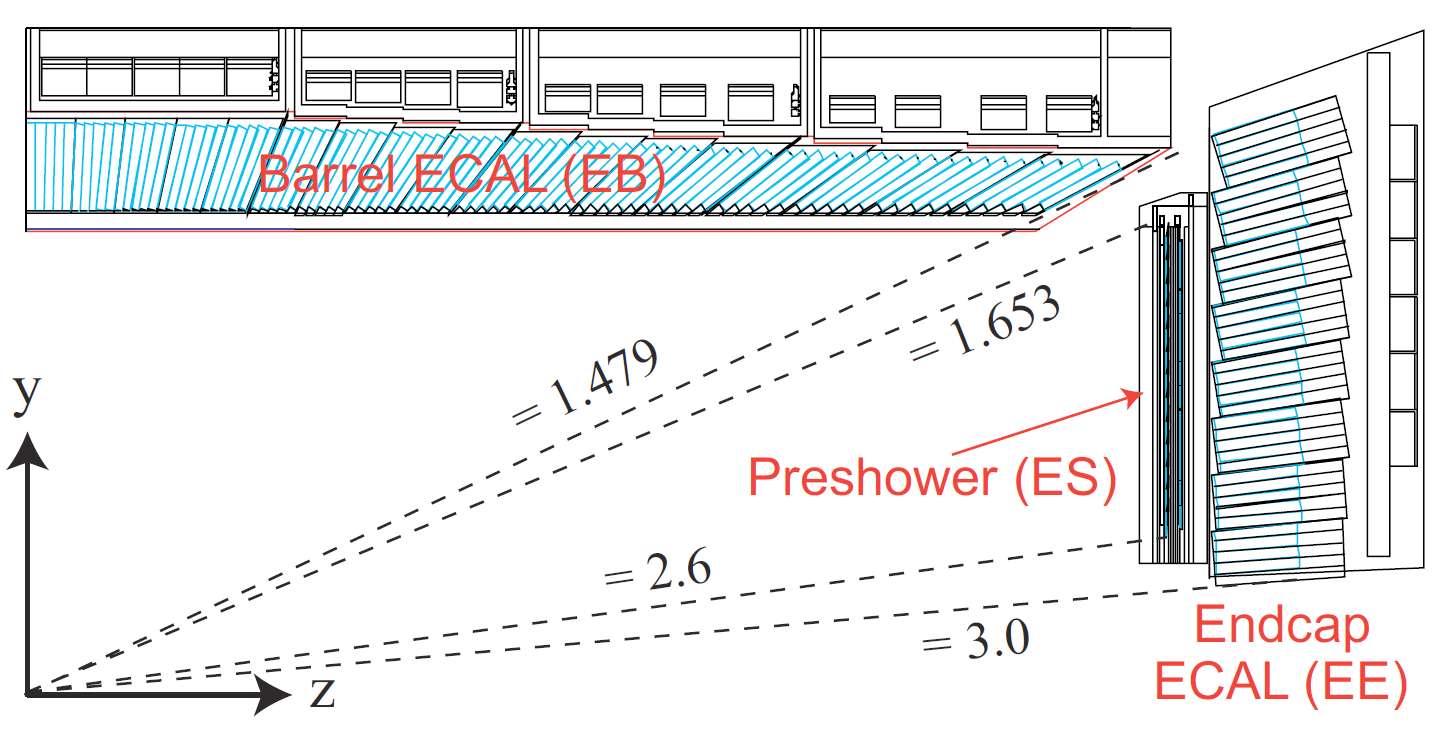
\includegraphics[angle=0,width=0.80\columnwidth]{fig/cms_ecal.png}
\end{center}
\caption{A cross section of the ECAL, showing its geometry and layout.~\cite{Isildak:2013kfa}}
\label{fig:cms_ecal}
\end{figure}

\end{subsection}

\begin{subsection}{Hadronic Calorimeter}
\label{subsec:hcal}

The primary purpose of the hadronic calorimeter (HCAL) is to measure the energy of hadrons, which can pass through the ECAL as they primarilly interact through the strong force.
The HCAL is a sampling calorimeter made up of either brass, iron, or steel absorbers and uses plastic scintillator tiles as the sampling material, which measures the energy of hadrons through scintillation, similarly to the ECAL:
As a hadron reaches through the HCAL, it interacts with one of the absorber layers, which results into a ``shower'' of particles that produces light in the scintillator tiles as the resulting particles pass through the sampling layers.
These light pulses are converted to electrical signals by optical fibers, which when summed have an amplitue proportional to the hadron's energy. 

\begin{figure}[tbp!]
\begin{center}
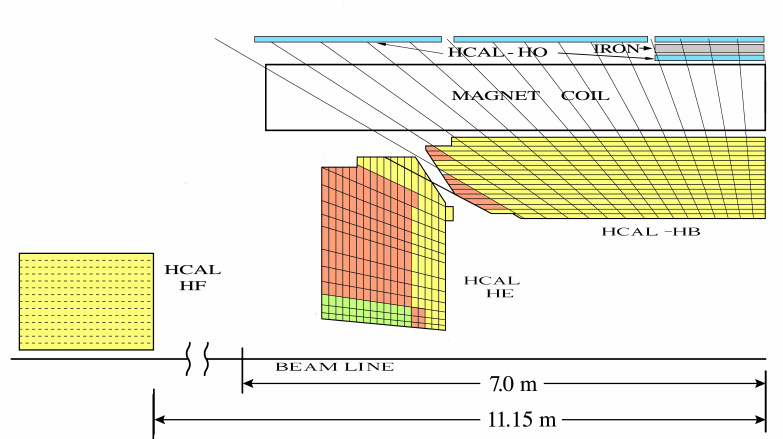
\includegraphics[angle=0,width=0.80\columnwidth]{fig/cms_hcal.png}
\end{center}
\caption{The layout and geometry of a quarter of the HCAL detector.~\cite{1748-0221-5-03-T03014}}
\label{fig:cms_hcal}
\end{figure}

The HCAL is separated into 4 components: the hadron barrel (HB), hadron endcap (HE), hadron forward (HF), and hadron outer (HO), the layouts of which are shown in Figure~\ref{fig:cms_hcal}.
The HB and HE completely surround the ECAL and were designed to minimize any cracks between the two subdetectors with the HB covering $|\eta|<1.3$ and the HE covering the rest up to $|\eta|=3$.
Both components function as sampling calorimteres with alternating absorber and sampling layers.
In the HB, the first and last layers are made of steel while the 14 other absorber layers are made of brass, while the HE is made up of 18 brass absorber layers.
For both components, there are sampling layers made of plastic scintillator tiles interspersed between each of the absorber layers.

The HF is used to measure the energy of the forward most hadrons in the pseudorapidity range of $3.0<|\eta|<5.0$.
At this forward position, the HF faces extradorinary levels of particle flux and had to be designed to handle this radiation.
Due to this constraint, the HF uses quartz fibers instead of plastic scintillator tiles as its active medium, as the quartz fiber are more radiation hard.
The HF uses both long fibers, which run the full depth ($165~\cm$) of the detector, and short fibers, which begin $22~\cm$ from the front end of the detector.
This geometry allows the HF to provide depth information of the energy deposits, which helps to identify electron and photons from hadrons, as the former tends to deposit most of its energy in the first depth, while the latter deposits its energy more equally between the two depths.
These fibers are embedded into the steel structure of the HF, which also acts as the absorber.

Lastly is the HO, whose main purpose is to act as a ``tail catcher''. 
Due to the geometrical constraint that the HCAL fit within the CMS solenoid, the HB does not have enough material in the central $\eta$ region to adequately contain hadron showers.
So to provide extra sampling layers, the HO sits just beyond the solenoid and has 1 to 2 scintillator layers and uses the magnet as an extra absorber layer. 
At this position, the HO is able to identify late starting showers and measure the amount of energy that is deposited past the HB.

\end{subsection}

\begin{subsection}{Muon System}

Muons, as implied by the ``M'' in CMS, are a central focus of the CMS detector, and the responsibiilty of identifying muons with high purity and providing precise momenta measurements falls to the muon system.
To do this, the muon system is composed of three types of gaseous detectors, motivated by the need to cover a large area and varying radiation environments.
Figure~\ref{fig:cms_muonsys} shows the layout of the muon system within the CMS detector.

\begin{figure}[tbp!]
\begin{center}
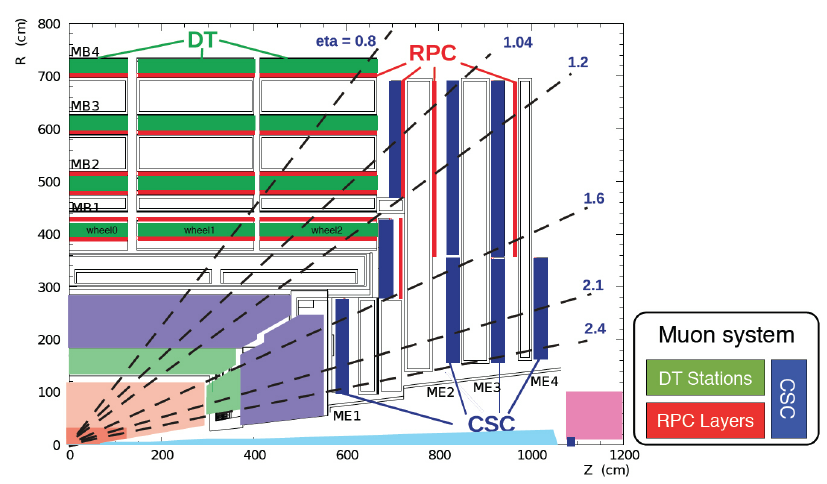
\includegraphics[angle=0,width=0.80\columnwidth]{fig/cms_muonsys.png}
\end{center}
\caption{The layout of the muon system within the CMS detector.~\cite{1748-0221-8-04-P04005}}
\label{fig:cms_muonsys}
\end{figure}

In the barrel region, $|\eta|<1.2$, drift tube chambers (DTs) are used as the neutron-induced background is small, the muon rate is small, and the magnetic field is uniform.
The DTs are organized into 4 stations, with three of the stations containing 8 chambers that measure position in the $r-\phi$ plane and 4 that measure position in the $z$-direction.
The last station only contains the 8 $r-\phi$ measuring chambers.
In the endcap regions of CMS, $0.9<|\eta|<2.4$, the expected muon and background rates are higher and the magnetic field is large and non-uniform, both of which preclude the use of DTs.
Instead, the muon system endcaps are instrumented with cathode strip chambers (CSCs) that have a high response time, fine segmentation, and higher radiation resistance
The CSCs have 4 stations in each endcap with chambers that are aligned perpendicular to the beam line and are able to provide measurements in the $r-phi$ plane and $z$-direction, along with the beam crossing time of a muon.

Both the DTs and CSC are capable of providing high efficiency and pure muon \pT triggers, independent of the rest of the detector.
But in order to further improve this, particularly at the full LHC luminosity, another complementary trigger system consisting of Resisitive Plate Chambers (RPCs) was added to both the the barrel and endcap regions ($|\eta|$<1.6).
The RPCs are double-gap chambers that operate with a fast response and good time resolution.
The spatial resolution, however, is coarser than the DTs or CSCs, though the extra hits in the RPC still help resolve ambiguities when making tracks.
There are a total of 6 RPC layers in the barrel muon system, which help improver triggers for low \pT muons, and 3 layers in each of the endcaps that help reduce background and improve the time and \pT resolution of muons.

\end{subsection}

\begin{subsection}{Trigger System}

The high instantaneous luminosity of the LHC provides many techincal challenges for the data aquisition system (DAQ), with proton-proton collissions occuring every $25~\ns$, corresponding to a frequency of $40~\mrm{MHz}$. 
At this collision rate, it is unfeasible to process and store the data for each event.
In order to reduce the rate, a two-stage trigger system is used to select only the most ``interesting'' events for processing.

The first stage is the Level-1 (L1) trigger system, which has approximately only $4~\mus$ to decide whether or not an event should be further processed. 
In order to operate at this timescale, the L1 trigger uses only coarse-grained information from the CMS calorimeters and the muon system.

For the calorimeter set of data, the L1 first generates trigger primitives by looking for lar for large energy deposits in the calorimter.
These trigger primitives are then passed to the Regional Calorimeter Trigger (RCT), which uses this information to determine electron/photon candidates and transverse energy sums per calorimeter region.
In addition, the RCT also calculates information relevant for detecting minimally ionizing particles, vetoing tau leptons, and muon isolation.
Lastly, the Global Calorimeter Trigger (GCT) uses the information from the RCT to construct jets and calculate the event-level transverse energy and missing transverse energy, along with the final isolated and non-isolated electron/photon candidates.

For the muon portion of the L1 trigger system, the DTs and CSCs both compute local trigger informationwhich consists of two- and three-dimensional track segments, respectively.
This information is then passed to a join DT-CSC track finder, which connects these segments into a full candidate track.
At the same time, the RPC constructs a separate, independent set of track candidates.
Both sets of candidate tracks are sent to the Global Muon trigger (GMT), which also takes in the relavent information from the RCT), to construct muon candidates.

Lastly, the candidate particles and event-level information from the GCT and GMT are sent to the Global Trigger, which takes this information and checks to see if certain criteria are met.
If so, a L1 Accept (L1A) is generated, which signals for the event to be fully read out.
This process, shown in Figure~\ref{fig:cms_trigger}, reduces the full readout rate to at most $100~\mrm{kHz}$.

\begin{figure}[tbp!]
\begin{center}
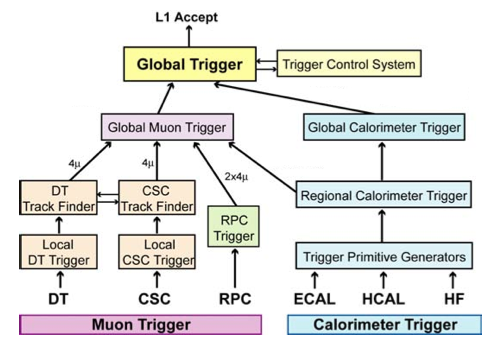
\includegraphics[angle=0,width=0.80\columnwidth]{fig/cms_trigger.png}
\end{center}
\caption{Flowchart depicting the generation of a L1 Accept.~\cite{1748-0221-3-08-S08004}}
\label{fig:cms_trigger}
\end{figure}

On the generation of an L1A, all the CMS subsystems read out their buffered data corresponding to the L1A event to the an event builder.
The data the event builder receives is both more complete and at a finer resolution, allowing it to construct more complex quantities before sending it to the High Level Trigger (HLT), the second stage of the trigger system.

The HLT software is run on a processor farm that reconstructs events in greater detail to decide whether or not they should be kept.
This framework is flexible as both the HLT software and the processor farm can be updated to meet changing experimental needs.
As such the exact criteria used by the HLT in its decision varies with time, but generally involves thresholding the \pT and/or multiplicity of particles along with event-level quantities, such as \HT.
At the end of this process, the trigger rate is at approximately $100~\mrm{Hz}$.

\end{subsection}

\end{section}

%Notes:
% include references for LHC and CMS (in intro to section)
% Add a physical view of the LHC (like a map view)
% Can expand by talking about how the beam is squeezed.
% Add an HF timing section

\chapter{Particle Reconstruction and Identification}
\label{chap:reco_id}
\begin{section}{Tracks}

Track reconstruction with the CMS detector faces many challenges, as at each bunch crossing $\mathcal{O}(10^3)$ particles are expected to pass through the CMS tracking system, all of which must be reconstructed in time to be inputted to the HLT.
This constraint makes it immensely challenging to attain high track-finding efficiency, while minimzing the number of fake tracks.

The first step of track reconstruction is to reconsutrct ``hits'' in a process called ``local reconstruction''.
In this step, signals in both the pixel and strip channels that are above some zero-suppression threshold are clustered together into hits, where the cluster positions and uncertainties are then estimated.

Next, tracks are reconstructed from these hits in order to provide estimates for the momentum and position of charged particles associated with the track.
This is done using specialized software based on Kalman filters known as Combinatorial Track Finder (CTF).
In order to reduce the combinatorial complexity of the problem, the CTF track reconstruction is performed six times. 
Each iteration attempts to reconstruct the most easily-identifiable tracks, e.g. high-\pT tracks, and then removes the hits associated with those tracks.
This helps simplify the track reconstruction in the following iterations.

Each iteration consists of four steps:
\begin{enumerate}
\item A seed is generated from a few (generally 2 or 3) hits. 
This seed provides an initial estimate of the trajectory and uncertainties associated with thet track.
\item A Kalman-based track finder is used to extrapolate seed trajectories along their expected paths. Additional hits that are compatabile with a path are assigned to that track candidate.
\item A track-fitting module uses a Kalman filter and smoother to provide estimates of the trajectory parameters for each track.
\item A track selection sets quality thresholds and discards tracks that fail the specified criteria.
\end{enumerate}

A detailed description of track reconstruction can be found in Reference~\cite{Chatrchyan:2014fea}.

\begin{subsection}{Vertices}

An essential part of event reconstruction is identifying which particles were produced at parton-parton interaction vertices (primary vertices) and which were produced at a decay vertex of produced particles (secondary vertices).
The process for selecting primary vertices consists of three steps: track selection, track clustering, and track fitting.

The track selection criteria is chosen in order to select tracks that are consistent with being produced promptly in the primary interaction region.
Tracks are required to have a small transverse impact parameter relative to the beam spot, a certain number of hits in the pixel and strip detectors, and good fit quality when fitting to the trajectory.
No requirement is placed on the \pT of tracks, in order to ensure a high reconstruction efficiency, even for minimum-bias events.

After the track selection, a deterministic annealing clustering algorithm~\cite{726788} is used in order to group together tracks that appear to originate from the same vertex.
Here the selected tracks are originally all assigned to the same vertex and are then slowly divided into multiple vertices.
This process continues until reaching a cutoff defined by balancing the risk of incorrectly splitting vertices and the resolving power of the algorithm.

Once the track clustering is completed, an ``adaptive vertex fitter'' is used to determine the 3D-position of vertices with at least two tracks~\cite{Fruhwirth:1027031}, in which tracks corresponding to a vertex are each assigned a probability of correctly belonging to the vertex.
The weighted sum of these probabilities is then used in the fitting algorithm to determine primary vertices.

In this process, many more than one primary vertex are reconstructed due to multiple parton-parton interactions in an event.
There is, however, usually only one primary vertex of interest in the event, corresponding to the primary vertex with the highest sum of track $\pT^2$.
This primary vertex is commonly referred to as \textit{the} primary vertex.
 
\end{subsection}

\end{section}

\begin{section}{Calorimeter Clusters}

Energy deposits in the various CMS calorimeters are clustered together to form ``calorimeter clusters''.
The purpose of the calorimeter clusters are to aid in,  detecting and measuring the energy and direction of stable neutral particles, separating these neutral particles from the energy deposits of charged hadrons, reconstructing and identifying electrons, along with their corresponding bremsstrahlung photons, and measuring the energy of charged hadrons with low-quality track parameters.

The calorimeter clustering is done in three steps. First, cluster seeds are identified as cells with an energy both larger than some threshold and larger than the energy of neighboring cells.
Next, these cluster seeds are formed into ``topological clusters'' by iteratively merging together neighboring cells that have significant energy deposits.
In this process, topological clusters can merge such that a cluster contains multiple cluster seeds.
Lastly, the energy in a topological cluster is distributed among its seeds through a Gaussian-mixture model that results in the final calorimeter clusters.

This clustering is performed separately in each subdetector calorimeter, including the ECAL preshower detector, whose two layers are treated independently.
There is no clustering performed in the HF, as each cell's short- and long-fibers measure the electromagnetic- and hadronic-energy components, as described in Subsection~\ref{subsec:hcal}.
These components directly give rise to ``HF EM'' and ``HF HAD'' clusters.

\end{section}

\begin{section}{Particle Flow}

The particle-flow (PF) algorithm is a holistic approach towards event reconstruction.
It combines the basic information of subdetectors, i.e. the tracks and clusters defined above, to identify each final-state particle and reconstruct their corresponding properties.
By correlating measurements from the tracker and calorimeter, the PF algorithm is able to provide improved energy and momentum measurements. A complete, detailed presentation of the particle-flow algorithm is given in~\cite{1748-0221-12-10-P10003,CMS-PAS-PFT-09-001,CMS-PAS-PFT-10-001}.

\begin{subsection}{Linking}

As a particle traverses through the CMS detector, it is expected to generate multiple input elements to the PF algorithm.
Thus, the first step of reconstructing particles is to ``link'' the various PF elements stemming from different subdetectors together.
This is done by defining a ``distance'' between two linked elements, where the closer the distance the more probable it is the two elements correspond to the same particle.
The linking algorithm then creates ``PF blocks'' by associating directly or indirectly linked elements together.
The exact criteria used to link elements together and define their distance depends on the type of elements being considered and are listed below.

A link between a track and calorimeter cluster is established by extrapolating the track trajectory through the ECAL and HCAL, up to a depth where energy deposits are most expected.
If the extrapolated track falls within the area of the calorimeter cluster, the two elements are linked and the link distance is defined as the separation between their positions in the $(\eta,\phi)$ plane.
In the case multiple clusters are linked to the same track only the link with the smallest distance is kept.

To link tracks with clusters from potential bremsstrahlung photons, tangents to the track are extrapolated to the ECAL.
If a tangent line falls within the cluster, the track and cluster are linked with the $\eta$-$\phi$ separation used as the link distance.

Calorimeter clusters in the HCAL, ECAL, and preshower detector are linked together when the position of a cluster in a more granular calorimeter (preshower or ECAL) is within the boundaries of a cluster with less granularity (ECAL or HCAL).
The distance between these two clusters is defined as either the $\eta$-$\phi$ or $x$-$y$ separation for HCAL-ECAL and ECAL-preshower links, respectively.
In the case where multiple HCAL(ECAL) clusters are linked to the same ECAL(preshower) cluster, only the link with the smallest distance is used.

Links between a track and a standalone-muon track, defined as a track segment constructed from hits in the muon system, are established when a global fit to the two tracks has an acceptable fit quality.
The link distance in this case is defined as the $\chi^2$ of the fit, and only the link with the smallest $\chi^2$ is retained when there are multiple links to the same standalone-muon track.
The resulting links are called ``global muons''.

\end{subsection}

\begin{subsection}{PF Reconstruction and Identification}

Once the PF blocks have been constructed, the PF algorithm is applied to reconstruct and identify a set of particles from each PF block.
This algorithm proceeds sequentially to hierarchically reconstruct particles as described below.

First, PF muons are formed from global muons whose momentum is compatible with that determined by only using the tracker.
The corresponding tracks are then removed from the PF block.

Next, PF electrons are identified by using information from the inner tracker and calorimters.
Electron candidates in a PF block are seeded by tracks with links to ECAL clusters.
These tracks are then re-extrapolated to the ECAL, and if a track is found to be compatible with ECAL energy deposits and consistent with an electron, the track and clusters are labelled a PF electron and are removed from the PF block.

The remaining elements in the PF block are used to form charged hadrons, photons, neutral hadrons, and, in rare cases, additional muons.
PF elements are identified as one of these particle-types by comparing the track momentum to the linked cluster energies.
The following scenarios define the identification process:

\begin{itemize}
\item If the total cluster energy is much smaller than the track momentum, the excess track momentum is labeled as a muon or fake track.
This occurs for less than 0.03\% of the tracks used in the algorithm.
\item If the total cluster energy agrees within the uncertainty of the track momentum, a PF charged hadron is formed.
The PF charged hadron is then assigned a mass equal to that of a charged pion and a momentum based on a fit of the tracker and calorimeter measurements.
\item If the total cluster energy is significantly larger than the track momentum and the excess is greater than the total ECAL energy, then the track is considered a PF charged hadron, as described above.
The excess ECAL energy is labeled a PF photon, and the remaining energy is assigned to a PF neutral hadron.
The excess ECAL energy is preferentially given to photons over neutral hadrons, as typically photons account for 25\% of the energy of a jet, while neutral hadrons only account for 3\%.
\item If the total cluster energy is significantly larger than the track momentum and the excess is less than the total ECAL energy, the track is considered a PF charged hadron and the excess calorimeter energy is assigned as a PF photon.
\item If there are ECAL or HCAL clusters without any linked tracks, the deposits are respectively treated as PF photons and PF neutral hadrons.
\end{itemize}

\end{subsection}

\end{section}

\begin{section}{Leptons}

As the identification criteria for selecting PF electrons and PF muons are weak, these objects serve as candidate particles. 
To increase the purity of true electrons/muon, more stringent criteria must be passed for a PF electron/muon to be considered an analysis-level electron/muon.
The number of analysis-level leptons, where a lepton is defined as either an electron or muon, is denoted as \Nleps.

\begin{subsection}{Electrons}

The electron candidates are required to have $\pT > 20~\GeV$, $|\eta| < 2.5$, and to satisfy identification criteria~\cite{electron_id} designed to remove hadrons misidentified as electrons, photon conversions, and electrons from heavy-flavor hadron decays. 
This criteria is shown in Table~\ref{tab:electron_id}, where $\sigma_{i\eta i\eta}$ is a variable based on the width of the electron shower shape, and $d_0$ and $d_z$ are the transverse and logitudinal impact parameters of the associated electron track, respectively.

\begin{table}[tb!]
\centering
\begin{tabular}{l|cc}
\hline \hline
Criteria                                          &  Barrel requirement  & Endcap requirement \\
\hline
$\sigma_{i\eta i\eta}$                            &  $< 0.0101$          &  $< 0.0283 $       \\
$\Delta\eta\mrm{(cluster,track)}$                 &  $< 0.0103$          &  $< 0.07333$       \\
$\Delta\phi\mrm{(cluster,track)}$                 &  $< 0.0336$          &  $< 0.114  $       \\
$E_{\text{hadronic}}/E_{\text{electromagnetic}}$  &  $< 0.876 $          &  $< 0.0678 $       \\
$\frac{1}{E} - \frac{1}{p}~[\GeV^{-1}]$           &  $< 0.0174$          &  $< 0.0898 $       \\
$|d_0|$~[mm]                                      &  $< 0.0118$          &  $< 0.0739 $       \\
$|d_z|$~[mm]                                      &  $< 0.373 $          &  $< 0.602  $       \\
Missing hits                                      &  $\leq 2  $          &  $\leq 1   $       \\
Pass photon conversion                            & True                 & True               \\
\hline \hline
\end{tabular}
\caption{Identification criteria that a PF electron must pass in order to be considered an analysis-level electron.}
\label{tab:electron_id}
\end{table}

Additionally, to preferentially select electrons that originate from the decay of W and Z bosons, electrons are required to be isolated from other PF candidates.
The relative isolation of a particle $I^{\mrm{rel}}$ is quantified using an optimized version of the mini-isolation variable $I_{\mrm{mini}}$.
Mini-isolation is computed as the scalar sum of the \pT of charged hadrons from the PV, neutral hadrons, and photons that are within a cone of radius $R^{\text{mini-iso}}$ surrounding the electron momentum vector $\vec{p}$ in $\eta$-$\phi$ space~\cite{Rehermann:2010vq}.
The cone radius $R^{\text{mini-iso}}$ varies with $1/\pT$ according to
\begin{align}
R^{\text{mini-iso}} &=\begin{cases} 0.2, &
\pT \leq 50\GeV \\
{10~\GeV}/{\pT}, & 50 < \pT \leq 200~\GeV \\
0.05, & \pT > 200~\GeV.
\end{cases}
\end{align}

The \pT-dependent cone size reduces the rate of accidental overlaps between the electron and jets in high-multiplicity events or highly Lorentz-boosted decays and in particular overlaps between bottom quark jets and leptons originating from a boosted top quark.
Relative isolation is computed as $I^{\mrm{rel}} = I_{\mrm{mini}}/\pT$ after subtraction of the average contribution from additional proton-proton collisions in the same bunch-crossing (pileup).
To be considered isolated, electrons must satisfy $I^{\mrm{rel}} < 0.1$.

The combined efficiency for the electron reconstruction, identification, and isolation requirements, shown in Figure~\ref{fig:electron_eff}, is about 50\% at $\pT$ of $20~\GeV$, increasing to 65\% at $50~\GeV$, and reaching a plateau of 80\% above $200~\GeV$~\cite{Khachatryan:2015hwa}.

\begin{figure}[tbp!]
\centering
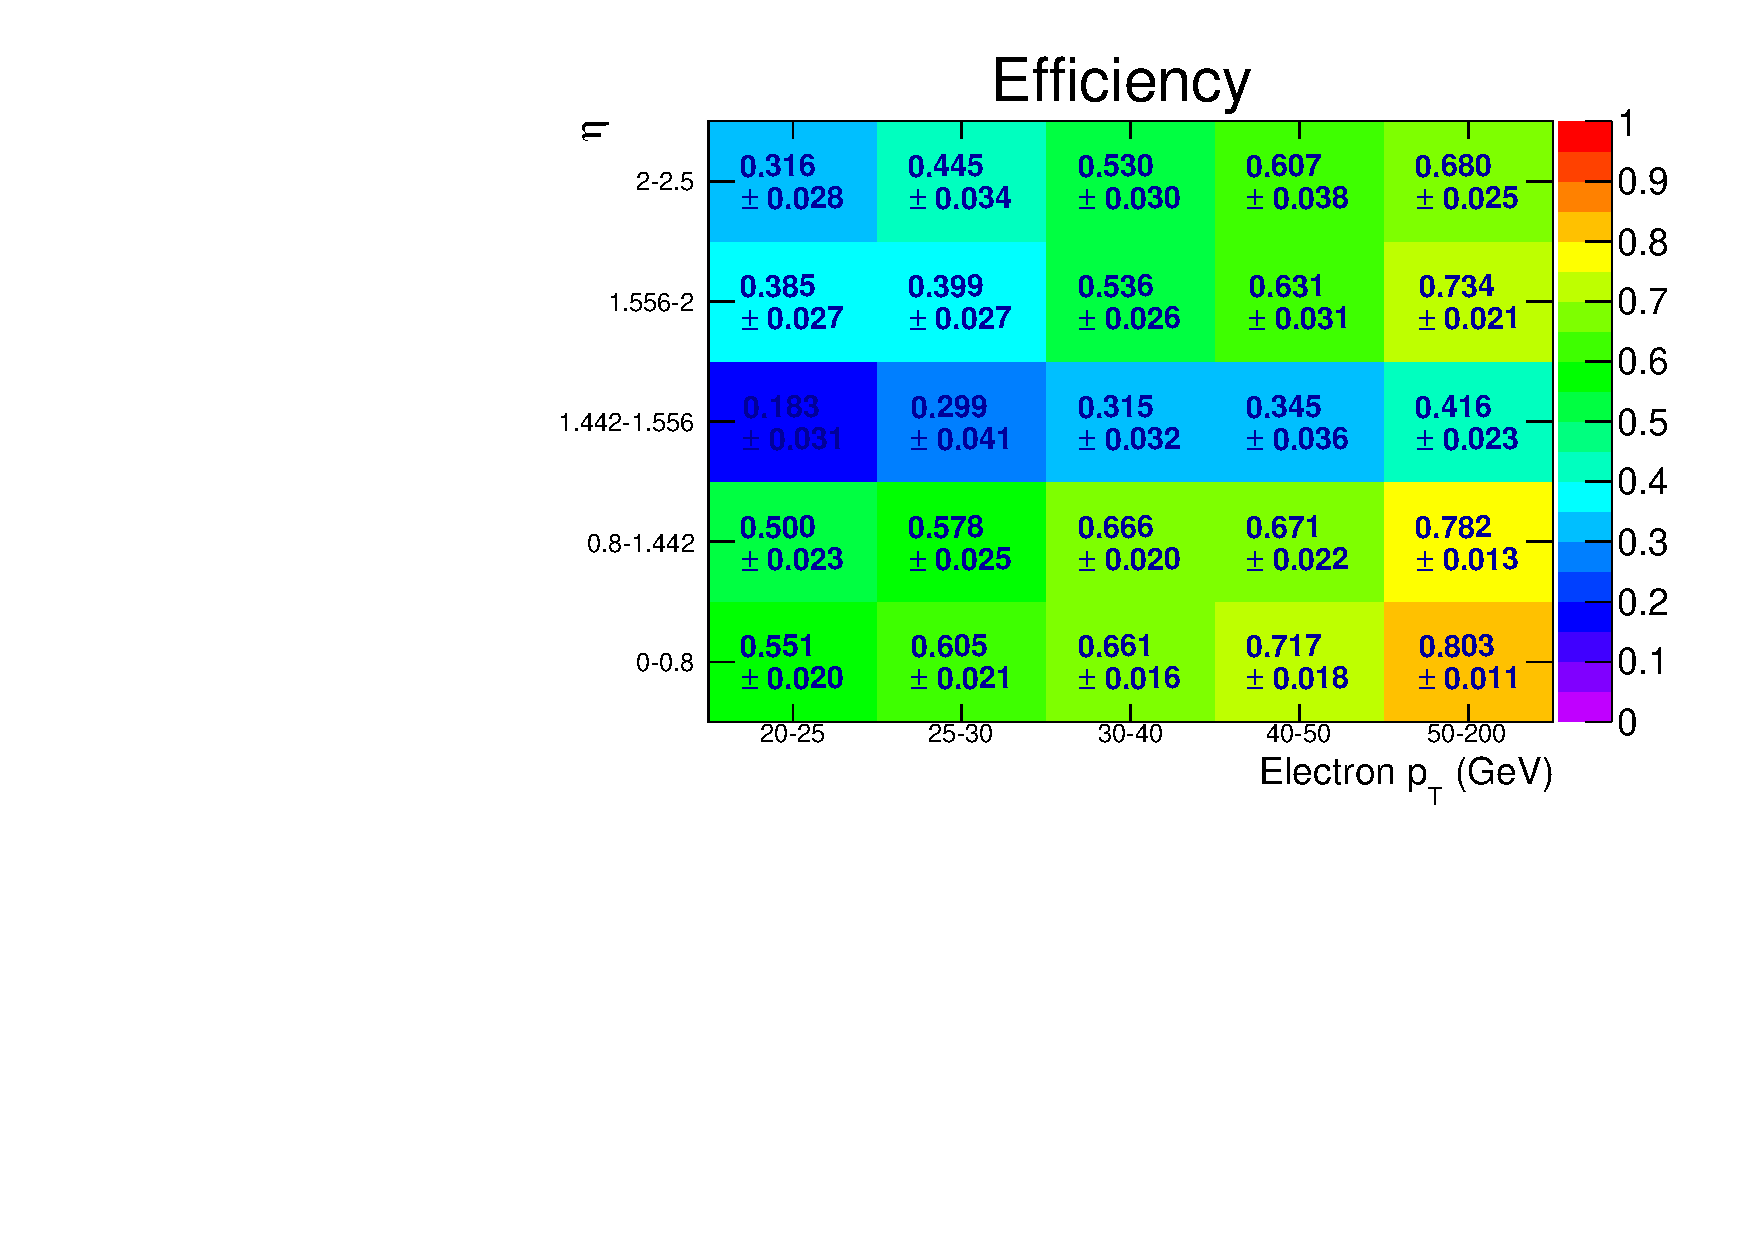
\includegraphics[angle=0,width=0.80\columnwidth]{fig/electron_eff.pdf}
\caption{The efficiency to select an analysis-level electron as a function of $\pT$ and $\eta$.
The low efficiency for $1.442 \leq |\eta| < 1.556$ corresponds to the ECAL ``crack'' region, the boundary between the EB and EE, in which electron reconstruction is particularly difficult.}
\label{fig:electron_eff}
\end{figure}

\end{subsection}

\begin{subsection}{Muons}

The muon candidates are required to have $\pT > 20~\GeV$, $|\eta| < 2.4$, and to satisfy identification criteria~\cite{muon_id} in order to select a high purity muon sample.
This criteria is shown in Table~\ref{tab:muon_id}, where $d_0$ and $d_z$ are the transverse and logitudinal impact parameters of the associated muon track, respectively.
Analogously to electron candidates, muon candidates are required to satisfy $I^{\mrm{rel}} < 0.2$, where the looser threshold is to account for purity differences between electrons and muons.

\begin{table}[tb!]
\centering
\begin{tabular}{l|c}
\hline \hline
Criteria                                       &  Requirement \\
\hline
Is PF muon                                     &  True        \\
Fraction of valid tracker hits                 &  $> 0.8$     \\
\hline
\multicolumn{2}{c}{\texttt{AND}}                              \\      
$|d_0|$~[mm]                                   &  $< 2$       \\
$|d_z|$~[mm]                                   &  $< 5$       \\
Is global muon                                 &  True        \\
Normalized global-track $\chi^2$               &  $< 3$       \\
$\chi^2$ of tracker-standalone position match  &  $< 12$      \\
Track-kink $\chi^2$                            &  $< 20$      \\
Segment compatibility                          &  $> 0.303$   \\
\multicolumn{2}{c}{\texttt{OR}}                               \\
Segment compatibility                          &  $> 0.451$   \\
\hline\hline
\end{tabular}
\caption{Identification criteria that a PF muon must pass in order to be considered an analysis-level muon.}
\label{tab:muon_id}
\end{table}

The efficiency for reconstructing muons, shown in Figure~\ref{fig:muon_eff} is about 70\% at $\pT$ of $20~\GeV$, increasing to 80\% at $50~\GeV$, and reaching a plateau of 95\% for $\pT > 200~\GeV$~\cite{Chatrchyan:2012xi}.

\begin{figure}[tbp!]
\centering
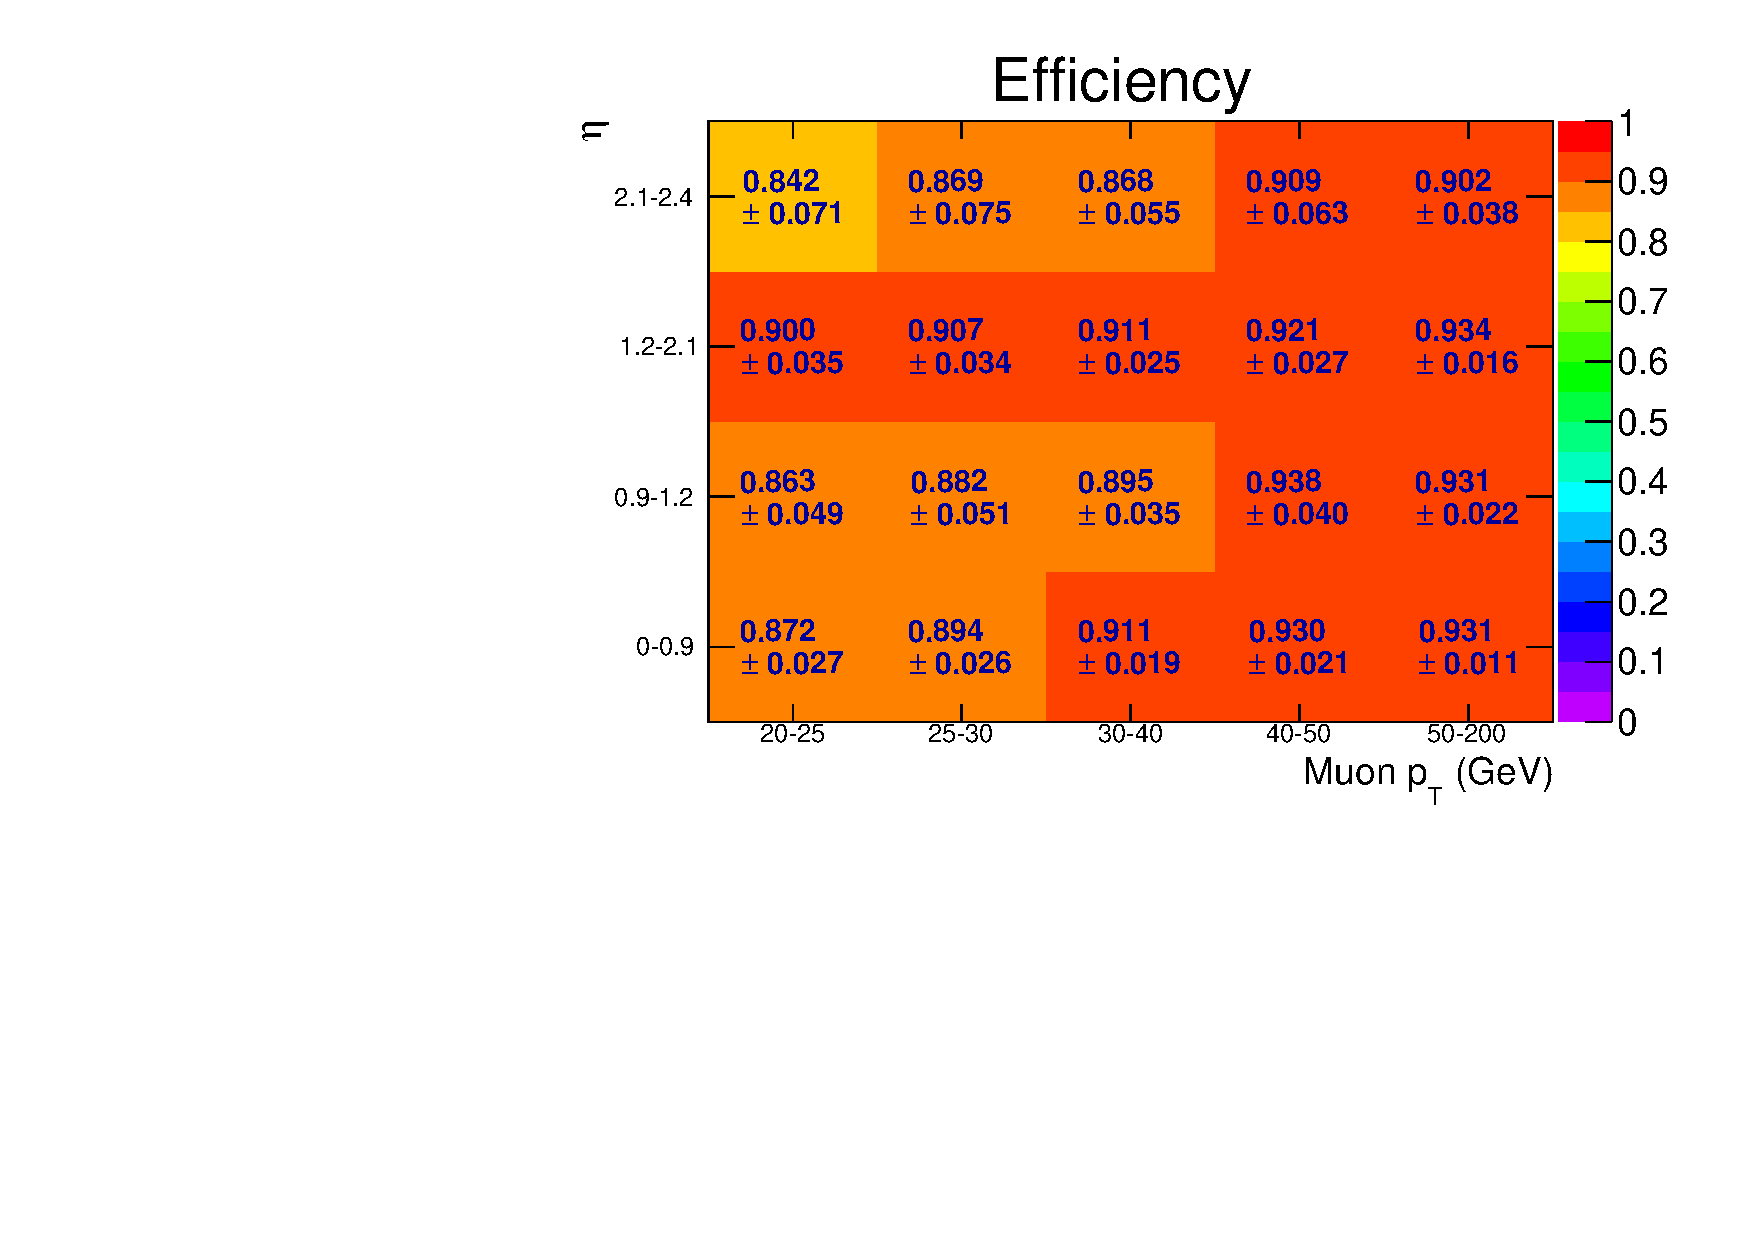
\includegraphics[angle=0,width=0.80\columnwidth]{fig/muon_eff.pdf}
\caption{The efficiency to select an analysis-level muon as a function of $\pT$ and $\eta$.}
\label{fig:muon_eff}
\end{figure}

\end{subsection}

\end{section}

\begin{section}{Jets}

When a quark or gluon is produced at the LHC, they quickly hadronize due to color confinement and produce a collimated ``spray'' of particles, called a jet, which is the direct detector observable.
The parameter of interest, however, is the momentum of the inital parton before hadronization.
Thus, clustering the constituent jet particles in a way that accurately reconstructs the inital parton momentum is essential.
Events, however, often contain multiple jets with each jet typically composed of some $\sim$$10$-$100$ particles that are incident on many detector channels across a large area.
This makes the problem of jet clustering non-trivial and an important aspect of object reconstruction.

\begin{subsection}{Clustering}

Jets are not physically-defined objects, and instead it is the clustering rules that define what a jet is.
The common class of clustering algorithms used are sequential recombination algorithms, which work by defining a distance measure between pairs of particles, typicaly based on energy and spatial-location, and then combining the closest pair of particles.
This process proceeds sequentially and ends when some threshold condition is met.

In particular, the distance measures, $d_{ij}$, which is the distance between two entities (particles or psuedojets), and $d_{iB}$, which is the distance between an entity and the beam, are often defined to be

\begin{equation}
d_{ij} = \mrm{min}(p_{\mrm{T}i}^{2n},p_{\mrm{T}j}^{2n})\frac{\Delta R_{ij}^{2}}{R^2},
\label{clustering_dij}
\end{equation}

\begin{equation}
d_{iB} = p_{\mrm{T}i}^{2n},
\label{clustering_diB}
\end{equation}
where $\Delta R_{ij}^{2} = \Delta \eta_{ij}^{2} + \Delta \phi_{ij}^2$, $R$ is the jet radius parameter that sets the scale of the jet's size, and $n$ is a parameter of the algorithm.
The clustering procedure then proceeds by finding the smallest of the distances, and if it is a $d_{ij}$, the two entities $i$ and $j$ are merged, while if it is a $d_{iB}$, entity $i$ is called a jet and is removed from the clustering list.

The parameter $n$ determines the clustering order of the algorithm and thus different choices for the value of $n$ lead to different clustering algorithms.
For $n = 1$, the clustering follows the \kT algorithm~\cite{Ellis:1993tq}, which prioritizes clustering softer particles first.
Setting $n = 0$, reproduces the Cambridge-Aachen algorithm~\cite{Dokshitzer:1997in}, which uses energy-independent clustering, relying only on the spatial distances between particles.
Lastly, choosing $n = -1$, gives the anti-\kT algorithm~\cite{Cacciari:2008gp}, which favors using the harder particles as the jet seeds and then clustering around them.
A more detailed discussion of jets, including a comparison of these and other clustering algorithms can be found in Reference~\cite{Salam:2009jx}.

\end{subsection}

\begin{subsection}{Selection}

The jets used in this dissertation are constructed by clustering PF candidates with the anti-\kT algorithm and $R = 0.4$, using the \textsc{FastJet} package~\cite{Cacciari:2011ma}.
To reduce the effect of pileup on the jet clustering and energy measurements, a process called ``Charged Hadron Subtraction'' is applied, where PF charged hadrons that do not originate from the PV are not included in the jet clustering.
In addtion, to remove the neutral energy component of pileup, the contribution from PF neutral hadrons produced by pileup is estimated based on the area of a jet and the energy density of the event and is subtracted from the jet~\cite{Cacciari:2007fd}.
Additionally, to prevent double-counting, any jets which contain a PF candidate identified as an analysis-level electron or muon are removed from the jet collection. 

Finally, to be considered an analysis-level jet, the jets must have $\pT > 30~\GeV$, $|\eta| < 2.4$, and must pass a set of loose identification requirements~\cite{jet_id,1748-0221-6-11-P11002} to surpress, for example, calorimeter noise.
These requirements are shown in Table~\ref{tab:jet_id}.
The resulting jets are considered to be ``\smallR'' jets  and the variable \Njets represents the number of these jets in an event.
Additionally, a proxy for the hadronic energy scale of an event, \HT, can be defined as
\begin{align}
\HT = \sum_{i = 1}^{\Njets} p_{T,i}^{jet}
\end{align}

\begin{table}[tb!]
\centering
\begin{tabular}{l|c}
\hline \hline
Criteria                          &  Requirement \\
\hline
Number of constituents            &  $> 1$       \\
Charged multiplicity              &  $> 0$       \\
Neutral electromagnetic fraction  &  $< 0.99$    \\
Neutral hadron fraction           &  $< 0.99$    \\
Charged electromagnetic fraction  &  $< 0.99$    \\
Chaged hadron fraction            &  $> 0$       \\
\hline\hline
\end{tabular}
\caption{Identification criteria that a jet candidate must pass in order to be considered an analysis-level jet.}
\label{tab:jet_id}
\end{table}

\end{subsection}

\begin{subsection}{b-tagging}

Jets that are formed through b-quark hadronization have several unique properties that allow them to be differentiated from jets formed through other quarks or gluons.
This ability to ``b-tag'' jets is a very useful tool for determining what physics processes occured in an event, as b~quarks are associated with specific physics process, such as top quark decays.
Similarly, many SUSY scenarios, where naturalness considerations motivate light third-generation squarks, result in either the direct or indirect production of b~quarks through the decay of SUSY particles.
Thus, b-tagging jets is not only often a crucial component to reducing backgrounds from processes where no b~quarks are expected, but also a powerful selector for potential signal events. 

This analysis uses the Combined Secondary Vertex v2 (CSVv2) algorithm~\cite{Chatrchyan:2012jua,Sirunyan:2017ezt}, which utilizes the long lifetimes, large masses, high-momentum daughter particles, and frequent semi-leptonic decays typical of b~hadrons to b-tag jets.
As the b~quark can only decay to an up or charm quark through highly Cabibbo surpressed weak interactions, b~hadrons tend to have long lifetimes, typically on the order of 150~\ps.
Because of this, b~mesons can travel a few mm to a cm from the PV before decaying and producing displaced tracks from which a secondary vertex can be reconstructed.
In addition, due to the relatively large b-quark mass, b~mesons tend to be heavy, which leads to both large secondary vertex masses and daughter particles with a hard momentum spectrum.
Lastly, the weak decay of the b~quark results in an associated electron or muon in about 20\% of decays.
The presence of these soft, nonisolated leptons provides an additional marker for the presence of a b-quark.

The CSVv2 algorithm exploits variables based on this information about secondary vertices, their associated displaced tracks, and the presence of soft leptons to accurately tag b-quark jets.
A selection of the variables used that have high discrimination are listed below:

\begin{itemize}
\item The significance of the flight distance in the transverse plane.
\item The number of SV
\item The SV mass
\item The number of tracks associated with the SV
\item The ratio of the transverse momentum of the SV tracks and the transverse momentum of the jet
\item The 3D impact parameter of soft leptons associated with the jet
\end{itemize}

These variables are then fed into a multilayer perceptron with one hidden layer that outputs a score between 0 and 1, indicating the likelihood the jet is a b-quark jet.
The distribution of CSVv2 discriminator values for different flavor jets is shown in Figure~\ref{fig:csv_discriminator}.

\begin{figure}[tbp!]
\centering
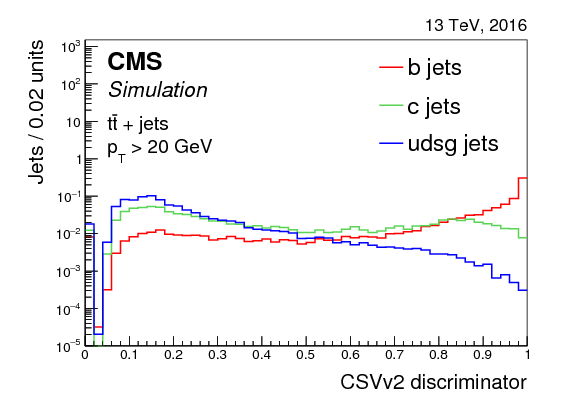
\includegraphics[angle=0,width=0.80\columnwidth]{fig/csv_discriminator.png}
\caption{The distribution of the CSVv2 discriminator values for jets of different flavors.
Jets are selected from \ttbar events and required to have $\pT > 20~\GeV$~\cite{Sirunyan:2017ezt}.}
\label{fig:csv_discriminator}
\end{figure}

A threshold score of 0.8484 is used to b-tag a jet and is chosen such that the mis-tag rate for light-flavor jets is 1\%.
This corresponds to a mis-tag rate for c-quark jets of 13--15\% (11--13\%) in the barrel (endcap) and a tagging efficiency for b~jets of 60--67\% (51--57\%) in the barrel (endcap) for jets with \pT between $30$-$50~\GeV$.
The tagging efficiency increases with \pT before decreasing to $\approx 50\%$ for jets above $150~\GeV$.
The b-tagging efficiency as a function of jet \pT is shown in Figure~\ref{fig:btag_eff}.

The number of b-tagged jets in an event is denoted as \Nb.

\begin{figure}[tbp!]
\centering
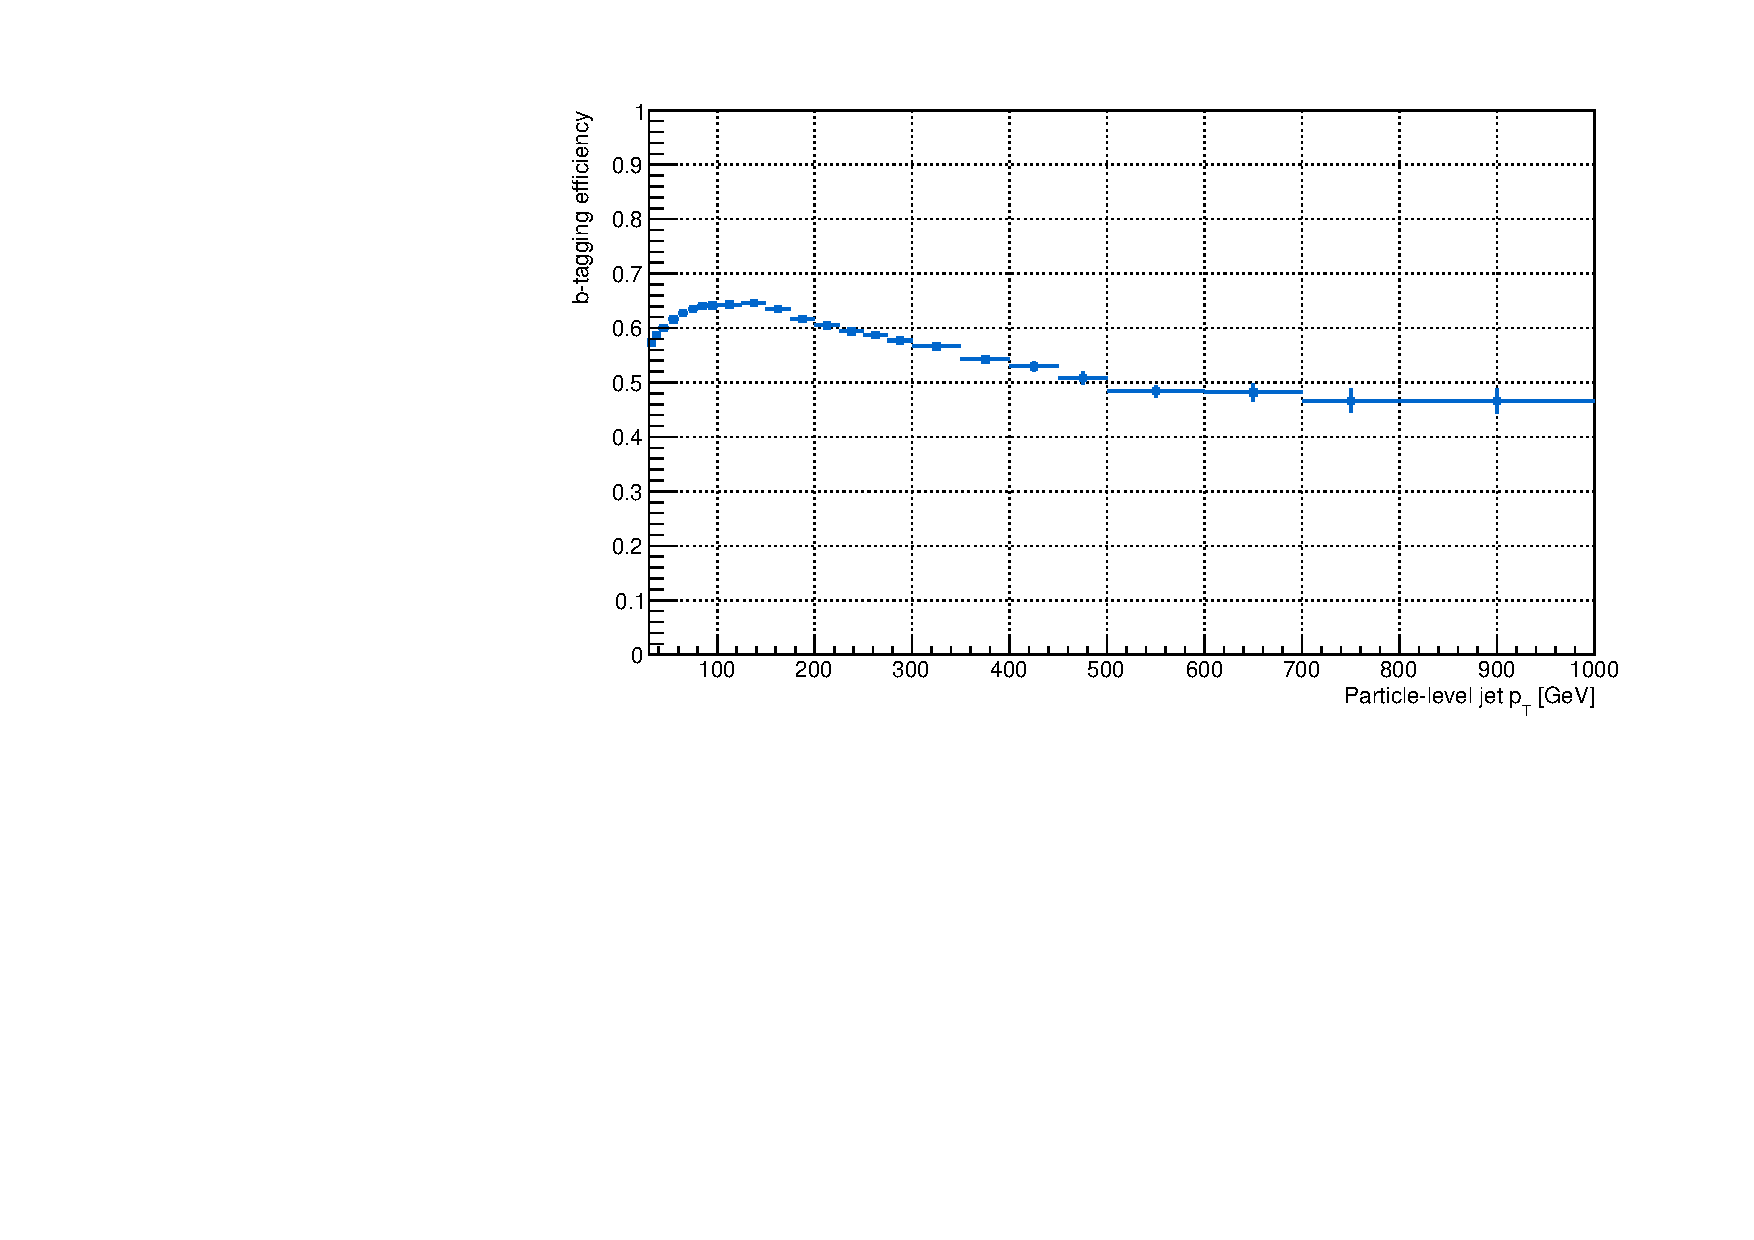
\includegraphics[angle=0,width=0.80\columnwidth]{fig/btag_eff.pdf}
\caption{The efficiency of the CSVv2 algorithm as a function of jet \pT at the working point used in this analysis.}
\label{fig:btag_eff}
\end{figure}

% SHOW VARIABLE PLOTS: https://inspirehep.net/record/1644362/plots

\end{subsection}

\end{section}

\begin{section}{Large-radius Jets}

While the distance parameter of \smallR jets is optimized for clustering the hadronization products of a single parton, it is often useful to exploit information of physical processes on a scale larger than a single jet, such as top quark or W boson decays.
One way to capture this information is to cluster jets with a large distance parameter, which encodes the momentum, angular, and multiplicity information of the partons contained in this larger jet.

In particular, this analysis constructs these ``\largeR'' jets by clustering ``\smallR'' jets with a distance parameter of $R = 1.2$.
Due to the relatively small number of \smallR jets in an event ($\lesssim 10$), the construction of these \largeR jets is insensitive to the clustering algorithm, and the anti-\kT algorithm is chosen.
While these \largeR jets could be constructed by performing the clustering at the PF candidate level, no significant improvement in performance was noted.
Thus, clustering \smallR jets were chosen for the following practical considerations.
First, the \textsc{FastJet} implementation of the anti-\kT algorithm has complexity $\mathcal{O}(n\log n)$~\cite{Cacciari:2005hq}, which results in a speed-up of on the order of 100x when clustering \smallR jets ($\lesssim 10$ objects) compared to PF candidates ($\sim$1000 objects).
Secondly, \largeR jets clustered from PF candidates would require the computation of new energy-measurement and pileup-removal calibrations for jets of this specific radius.
Small-$R$ jets, however, already incorporate standardized calibrations and by clustering these calibrated \smallR jets, the \largeR jets correspondingly incorporate corrections without the need of any additional development.

In addition to \smallR jets, the jets associated with selected leptons are included in the formation of \largeR jets in order to capture as much of an event's kinematic information as possible.
For example, this helps reduce the difference between \largeR jets formed by clustering hadronic and (semi-)leptonic decays, as by including the lepton, the only information difference between the two scenarios is due to the undetected neutrino(s).

This technique of clustering \smallR jets into \largeR jets has been used previously by both the ATLAS and CMS collaborations, e.g. References~\cite{Aaboud:2017aeu,Khachatryan:2016uwr}.

\begin{subsection}{\MJ\,--- The Sum of Large-radius Jet Masses}
\label{subsec:MJ}

A measure of the mass-scale of an event, \MJ, can be constructed by summing the masses of large-radius jets, defined as
\begin{align}
\MJ = \sum_{J_{i}\, \in\, {\text{large-}R\text{ jets}}} m(J_i)
\end{align}
where $m(J)$ is the mass of a single \largeR jet.

The quantitity \MJ has significant discriminating power between SM background processes and signal processes, as SM events tend to have significantly lower mass-scales than signal events that involve high mass particles.
For example, \MJ in events with only a produced \ttbar pair is limited to be $\lesssim 2m_{top} \approx 350~\GeV$.
This is because the top quarks decay back-to-back and if each top quark's decay products are captured in a single \largeR jet, two \largeR jets are clustered each with $m(J) = m_{top}$, resulting in $\MJ = 2m_{top}$.
In the case where a top quark is not fully contained in a \largeR jet, the mass of that \largeR jet, and correspondingly \MJ, is even smaller.
For signal events, however, the mass-scale is roughly set by the gluino mass, which is on the order of $1~\TeV$.

The \MJ distribution in \ttbar and signal events with $\mglu = 1000~\GeV$ and $1600~\GeV$, selected with a $\Njets \geq 8$ requirement to ensure both processes have similar \Njets distributions, is shown in Figure~\ref{fig:mj_distributions}. 
From the figure, it can be seen that the \MJ distribution gets increasingly harder with higher gluino mass.
Also of note is that the \MJ distribution in \ttbar events extends past $2m_{top}$.
This is because, in the presence of significant ISR, the ISR jets can either overlap with the \ttbar daughter jets or boost the \ttbar system such that the system is collimated, both which result in high-mass \largeR jets and, correspondingly, high-\MJ.
Processes of this nature are responsible for generating high \MJ background events.

The quantity \MJ was proposed in phenomenological studies~\cite{Hook:2012fd,Cohen:2012yc,Hedri:2013pvl} and was first used for RPC SUSY searches by the ATLAS Collaboration in all-hadronic final states~\cite{Aad:2015lea,Aad:2013wta} and by the CMS Collaboration in single-lepton events~\cite{Khachatryan:2016uwr,Sirunyan:2017fsj}.
Additionally, the basic properties and performance of the \MJ variable were commissioned using early $\sqrt{s} = 13~\TeV$ data~\cite{CMS-DP-2015-035}.

\begin{figure}[tbp!]
\centering
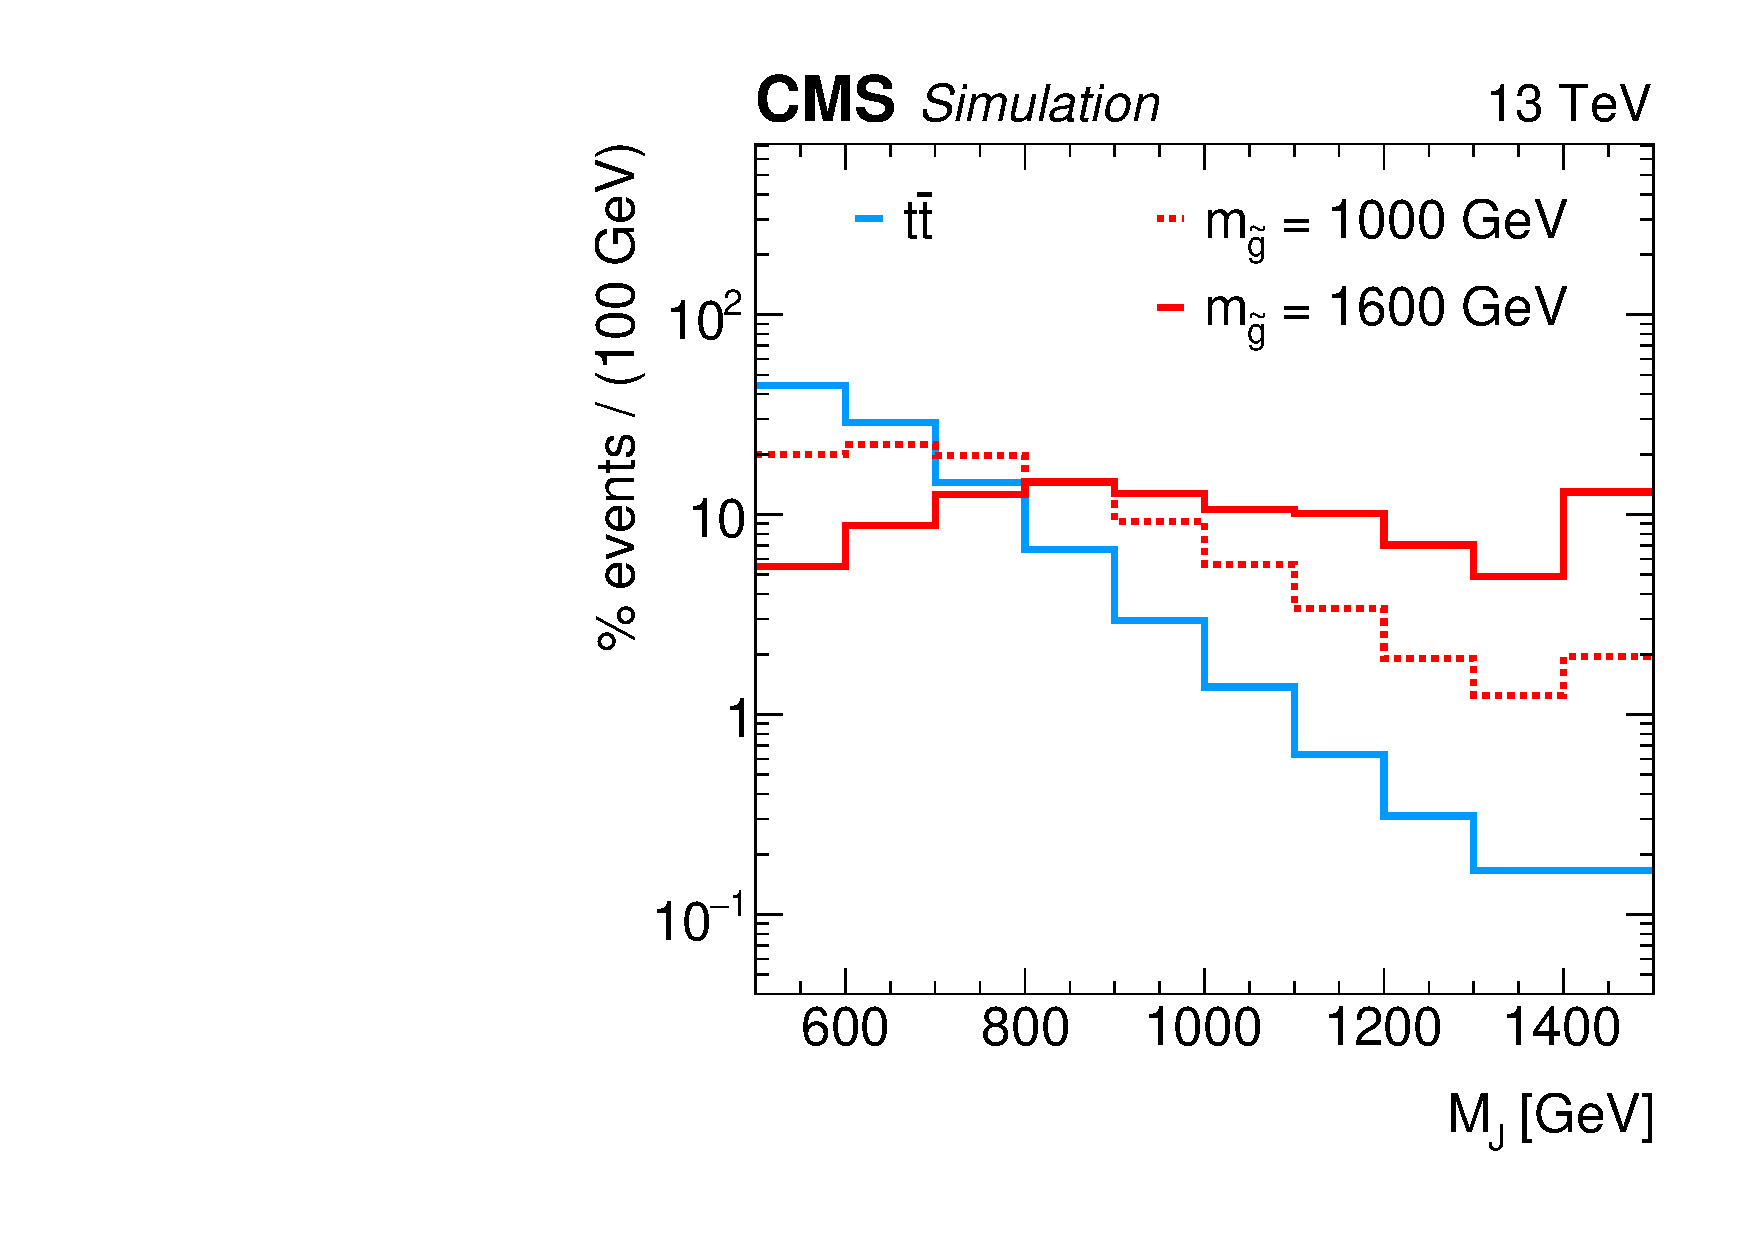
\includegraphics[angle=0,width=0.80\columnwidth]{fig/mj_distributions.pdf}
\caption{Distributions of \MJ, normalized to the same area, for \ttbar events and signal events with $\mglu = 1000~\GeV$ and $1600~\GeV$ in a selection of \baseNleps, \baseHT, $\Njets \geq 8$, \baseMJ, and \baseNb.}
\label{fig:mj_distributions}
\end{figure}

\end{subsection}

\end{section}

\part{Data, Simulation, and Selection}
\chapter{Samples}
\begin{section}{Section Title}

Lorem ipsum dolor sit amet, consectetur adipiscing elit, sed do eiusmod tempor incididunt ut labore et dolore magna aliqua. Ut enim ad minim veniam, quis nostrud exercitation ullamco laboris nisi ut aliquip ex ea commodo consequat. Duis aute irure dolor in reprehenderit in voluptate velit esse cillum dolore eu fugiat nulla pariatur. Excepteur sint occaecat cupidatat non proident, sunt in culpa qui officia deserunt mollit anim id est laborum.

\end{section}

\chapter{Event Selection}

\begin{section}{Baseline selection}

One of the main challenges for a SUSY search is that the ratio of SM events to SUSY events is (ROUGHLY) 10 billion to 1.
To surmount this problem, it is paramount to develop highly efficient signal-to-background discriminators.
Luckilly, SUSY signatures typically have characteristics unlike most SM processes.
In particular, for the T1tbs process, events are expected to have a large number of jets, many of which are b-quark jets, resulting in large amount of hadronic energy.
Additionally, the mass scale of the event is expected to be larger than most SM events due to the high masses of the gluinos (i.e. \~1~\TeV).
These features are used to construct the ``baseline selection'', defined as a set of requirements that events must pass in order to be included in the analysis.
Here the baseline selection is defined as $\Nleps=1$, $\MJ>500~\GeV$, $\HT>1200~\GeV$, $\Njets\geq4$, and $\Nb\geq1$.
Figure~\ref{nminus1} shows the ``N-1'' distributions of these variables, which are plots showing the 1D distribution of a variable with the baseline selection applied, except for the requirement corresponding to the plotted variable.
Figure~\ref{cutflow} shows a ``cutflow'' table, which depicts the expected yields for each process as each requirement of the baseline selection is indiviually applied.
Note that this analysis explicitly requires exactly 1 lepton (defined as a muon or electron).
As can be seen in 0-lepton bin of the N-1 plot of \Nleps, there is still significant amounts of QCD production compared to the expected signal yield.
Requiring exactly 1 lepton reduces the background by XX\%, while only reducing the signal by YY\% compared to being inclusive in \Nleps.
An additional benefit of this selection is that the SM backround is dominated by a single process (\ttbar), which reduces the complexity of the background prediction.
Including additional \Nleps regions is being investigated for future iterations of the analysis.
A final note of interest is that there is no requirement on the \MET, making this analysis sensitive to BSM models other than RPV SUSY that produce either little or no \MET in an event.

A final requirement for the baseline selection is that events must pass a series of filters designed to remvoe poorly reconstructed events. These standard filters remove events with noise in the HCAL or ECAL, beam halo effects, jets that fail to pass quality criteria, and events with zero good primary vertices.

\end{section}

\begin{section}{Trigger}
% Story doesn't flow well. Information is out of order.
In order to select events in data that pass the baseline selection, events are required to either have an online-\HT of at least 900 \GeV or at least one jet with online-\pT above 450~\GeV.
Figure~\ref{trigger} shows the performance of the trigger during the first XX~\ifb (Runs B-G) and the remaining YY~\ifb (Run H).
During Runs B-G the trigger plateaus at YYYY~\GeV with 100\% efficiency, during Run H, however, a bug in the trigger implementation caused very high-\pT jets to not be included in the online-\HT calculation, which resulted in a significantly plateau efficiency of YY\%.
In order to recover the lost efficiency, a trigger requiring at least one jet with online-\pT above 450~\GeV is ``OR'''d with the \HT trigger
With this addition, the trigger effieciencies for background and signal are >99\% for events with \HT>1200~\GeV, as shown in Figure~\ref{ORtriggers}.

\end{section}

\begin{section}{Analysis Binning}
After the baseline selection, the background is dominated by \ttbar events with small contributions from \Wjets and QCD production.
There are additional rare background processes, jointly noted as ``Other'', with tiny, but non-zero contributions that arise from single top quark, \ttW, \ttZ, \ttH, \tttt, and Drell-Yan production.

In order to further increase the signal-to-background ratio, as well as create background-dominated control regions, the analysis region is binned with respect to \Njets and \MJ. 
The \Njets bins are defined as $4 \leq \Njets \leq 5$, $6 \leq \Njets \leq 7$, and $\Njets \geq 8$.
Each \Njets bin is further split into bins of $500 < \MJ \leq 800~\GeV$, $800 < \MJ \leq 1000~\GeV$, and $\MJ > 1000~\GeV$, with the exception of the $4 \leq \Njets \leq 5$ bin for which the two highest \MJ bins are combined due to the limited data sample size in the $\MJ \geq 1000~\GeV$ bin.
A diagram representing this binning is shown in Figure~\ref{fig:analysis_regions}
The low-\Njets, low-\MJ bins are expected to be background-dominated and are used as control regions for constraining sytematics and for validating the prediction methodology, while the high-\Njets, high-\MJ bins.

\begin{figure}[tbp!]
\centering
  \begin{tabular}{ |c|c|c|c| }
    \hline
%    \multirow{2}{*}{\MJ [\GeV]} & \multicolumn{3}{c|}{\Njets} \\ \cline{2-4}
%                                         & 4--5                & 6--7  & $\geq$8   \\ \hline
%    500--800                             & CR                  & CR    & SR        \\ \hline
%    800--1000                            & \multirow{2}{*}{CR} & SR    & SR        \\ \cline{1-1} \cline{3-4}
%    $>$1000                              &                     & SR    & SR        \\ \hline
  \end{tabular}
  \caption{\label{fig:analysis_regions} Illustration depicting the (\Njets, \MJ) binning after the baseline selection, with control and signal region bins denoted by ``CR'' and ``SR'', respectively.}
\end{figure}

Within each \Njets and \MJ bins, the \Nb distribution is examined for evidence of new physics and is separated into bins of $\Nb=1$, 2, 3, and $\geq 4$.
The two lowest \Nb bins are used to provide constraints on the background normalizations and systematic uncertainites, while the higher \Nb bins are the most sensitive to potential signals due to its larger signal-to-background ratios.

In total, this analysis has 8 kinematic regions--3 control and 5 signal regions with four \Nb bins per kinematic region.

\end{section}

\part{The Search}
\chapter{Background Prediction}
\begin{section}{Overview}

This analysis seeks to find evidence of new physics by searching for deviations from the SM in the \Nb distribution.
In order to do this, it is essential to be able to robustly and accurately predict both the normalization and shape of the \Nb distribution.
To obtain these predictions, a global maximum-likelihood fit is performed.
This fit is carried out both for a background-only hypothesis and for signal-plus-background hypotheses, in which a signal contribution is extracted in addition to the contributions of SM background processes.
The model is constructed using the poisson probabilities of the bin contents of the \Nb distribution for all \Njets, \MJ regions, while systematic uncertainties are applied as nuisance parameters.

As the kinematic tails of the \Njets and \MJ variables are difficult to model reliably, the \ttbar and QCD normalizations are individually allowed to (almost) freely vary in each (\Njets, \MJ) bin.
The \ttbar normalizations are constrained in each bin by the low-\Nb bins, while the QCD normalizations are constrained by control regions with no identified leptons ($\Nleps = 0$).
The overall \Wjets normalization is determined from data and is allowed to vary across \Njets bins by amounts measured using a kinematically similar \Zjets sample, while the normalization of Other is largely taken from simulation, as its contribution is small in the regions considered.
Further details on the measurement of the normalizations are given in the following sections.

Once the SM backround processes are normalized accordingly, further corrections to the \Nb shape are relatively small.
The nominal \Nb shape prediction for each process is taken from simulation with data-to-simulation correction factors (SFs) applied for the tagging efficiency of heavy- and light-flavor jets~\cite{Chatrchyan:2012jua,BTV-16-002}.
This shape is allowed to vary in order to assess the impact of mismodeling of relevant parameters, such as the rate of gluon splitting to \bbbar and the b-tagging SFs.
The appropriate ranges for these parameters are determined based on measurements in dedicated control samples and then constrained by a simultaneous fit across all bins of \Njets and \MJ in a correlated manner.
A detailed discussion of these variations and their measurements is given in~\ref{Systematis Uncertainties}.

\end{section}

\begin{section}{\ttbar and QCD Normalizations}

The \ttbar and QCD normalizations are allowed to float in each (\Njets, \MJ) bin but with a loose constraint across \MJ bins discussed in the following subsection.
The largest constraint on the \ttbar normalization in each bin is the background-dominated $\Nb \leq 2$ bins, while the QCD normalization in each bin is mostly constrained by corresponding bins in a similar 0-lepton kinematic region selected by requiring $\Nleps = 0$, $\HT > 1500~\GeV$, $\MJ > 500~\GeV$, $\Njets \geq 6$, and $\Nb \geq 1$.
The higher \HT requirement compared to the analysis's baseline selection is imposed in order to account for the extra energy in an event carried by the lepton in the $\Nleps = 1$ selection, while the higher \Njets selection is imposed in order to account for differences in the \Njets distribution between the $\Nleps = 1$ and $\Nleps = 0$ samples.
This control sample follows the same kinematic binning as the $\Nleps = 1$ regions, except that the \Nb distribution in each bin is integrated in \Nb for $\Nb \geq 1$ and each bin's \Njets requirement is increased by 2.
A diagram representing the binning of the $\Nleps = 0$ control sample is shown in Figure~\ref{fig:nlep0_regions}
The QCD contribution in a particular $\Nleps = 1$ bin is then constrained by the corresponding $\Nleps = 0$ bin.
To avoid biasing the normalization measurement, the small contribution of \ttbar background to the $\Nleps = 0$ control regions is included using the normalization from the corresponding $\Nleps = 1$ bins, while contributions from other processes are taken from simulation.

\begin{figure}[tbp!]
\centering
\begin{tabular}{ |c|c|c|c| }
\hline
%\multirow{2}{*}{\MJ [\GeV]} & \multicolumn{3}{c|}{\Njets} \\ \cline{2-4}
%                                     & 4--5                & 6--7  & $\geq$8   \\ \hline
%500--800                             & CR                  & CR    & SR        \\ \hline
%800--1000                            & \multirow{2}{*}{CR} & SR    & SR        \\ \cline{1-1} \cline{3-4}
%$>$1000                              &                     & SR    & SR        \\ \hline
\end{tabular}
\caption{Diagram depicting the (\Njets, \MJ) binning of the $\Nleps = 0$ QCD control region.}
\label{fig:nlep0_regions}
\end{figure}

\begin{subsection}{\MJ Connection}

Due to the large freedom of unconstrained normalization parameters, the fit can be sensitive to rare statistical fluctuations and return unphysical normalization values particurlarly in bins dominated by \ttbar events.
For example, in psuedodata experiments, where data are generated according to the statistical and systematic uncertainties of the pre-fit values, the fit reduced the \ttbar contribution in the $\Njets \geq 8$, $\MJ > 1000~\GeV$ bin (where statistical uncertainties are largest) to $\sim0$ in about $\sim1\%$ of the experiments.
This can be seen in Figure~\ref{fig:mj_connection_exps} (left) which shows a low tail in the distribution of post-fit \ttbar yields in the $\Njets \geq 8$, $\MJ > 1000~\GeV$ bin for 1,000 psuedodata experiments.
When yields in a bin have a large fluctuation downwards, the fit must lower the normalization of a process to compensate.
The QCD, \Wjets, and Other contributions, however, are largely constrained by other data control samples or taken from simulation, and so the fit uses the freedom to adjust the \ttbar normalization in order to compensate for the fluctuation, leading to the unphysically small values.

In order to avoid this instability, the normalizations of \ttbar and QCD are (independently) connected by log-normal constraints between adjacent \MJ bins.
By correlating the normalizations across \MJ bins, the fit's sensitivity to large fluctuations in a single bin is greatly reduced.
The size of these connections is motivated by measurements of the data-to-simulation ratio with $\Nb = 1$ events (in order to avoid potential signal contamination) and is particuarly chosen to be significantly larger than the uncertainty on the data-to-simulation ratios in order to avoid over-constraining the normalization parameters, while still providing some constraint against unphysical fits.
Based on these measurements, shown in Figure~\ref{fig:mj_connection}, and criteria, a connection size between adjacent bins of [50\%-200\%] is chosen.

Figure~\ref{mj_connection_exps} (right) shows the results of the same 1,000 psuedodata experiments but now with this constraint across \MJ bins applied.
The resulting distribution of post-fit \ttbar yields now shows no evidence of unphysical normalizations and appears to be better behaved.

\begin{figure}[tbp!]
\centering
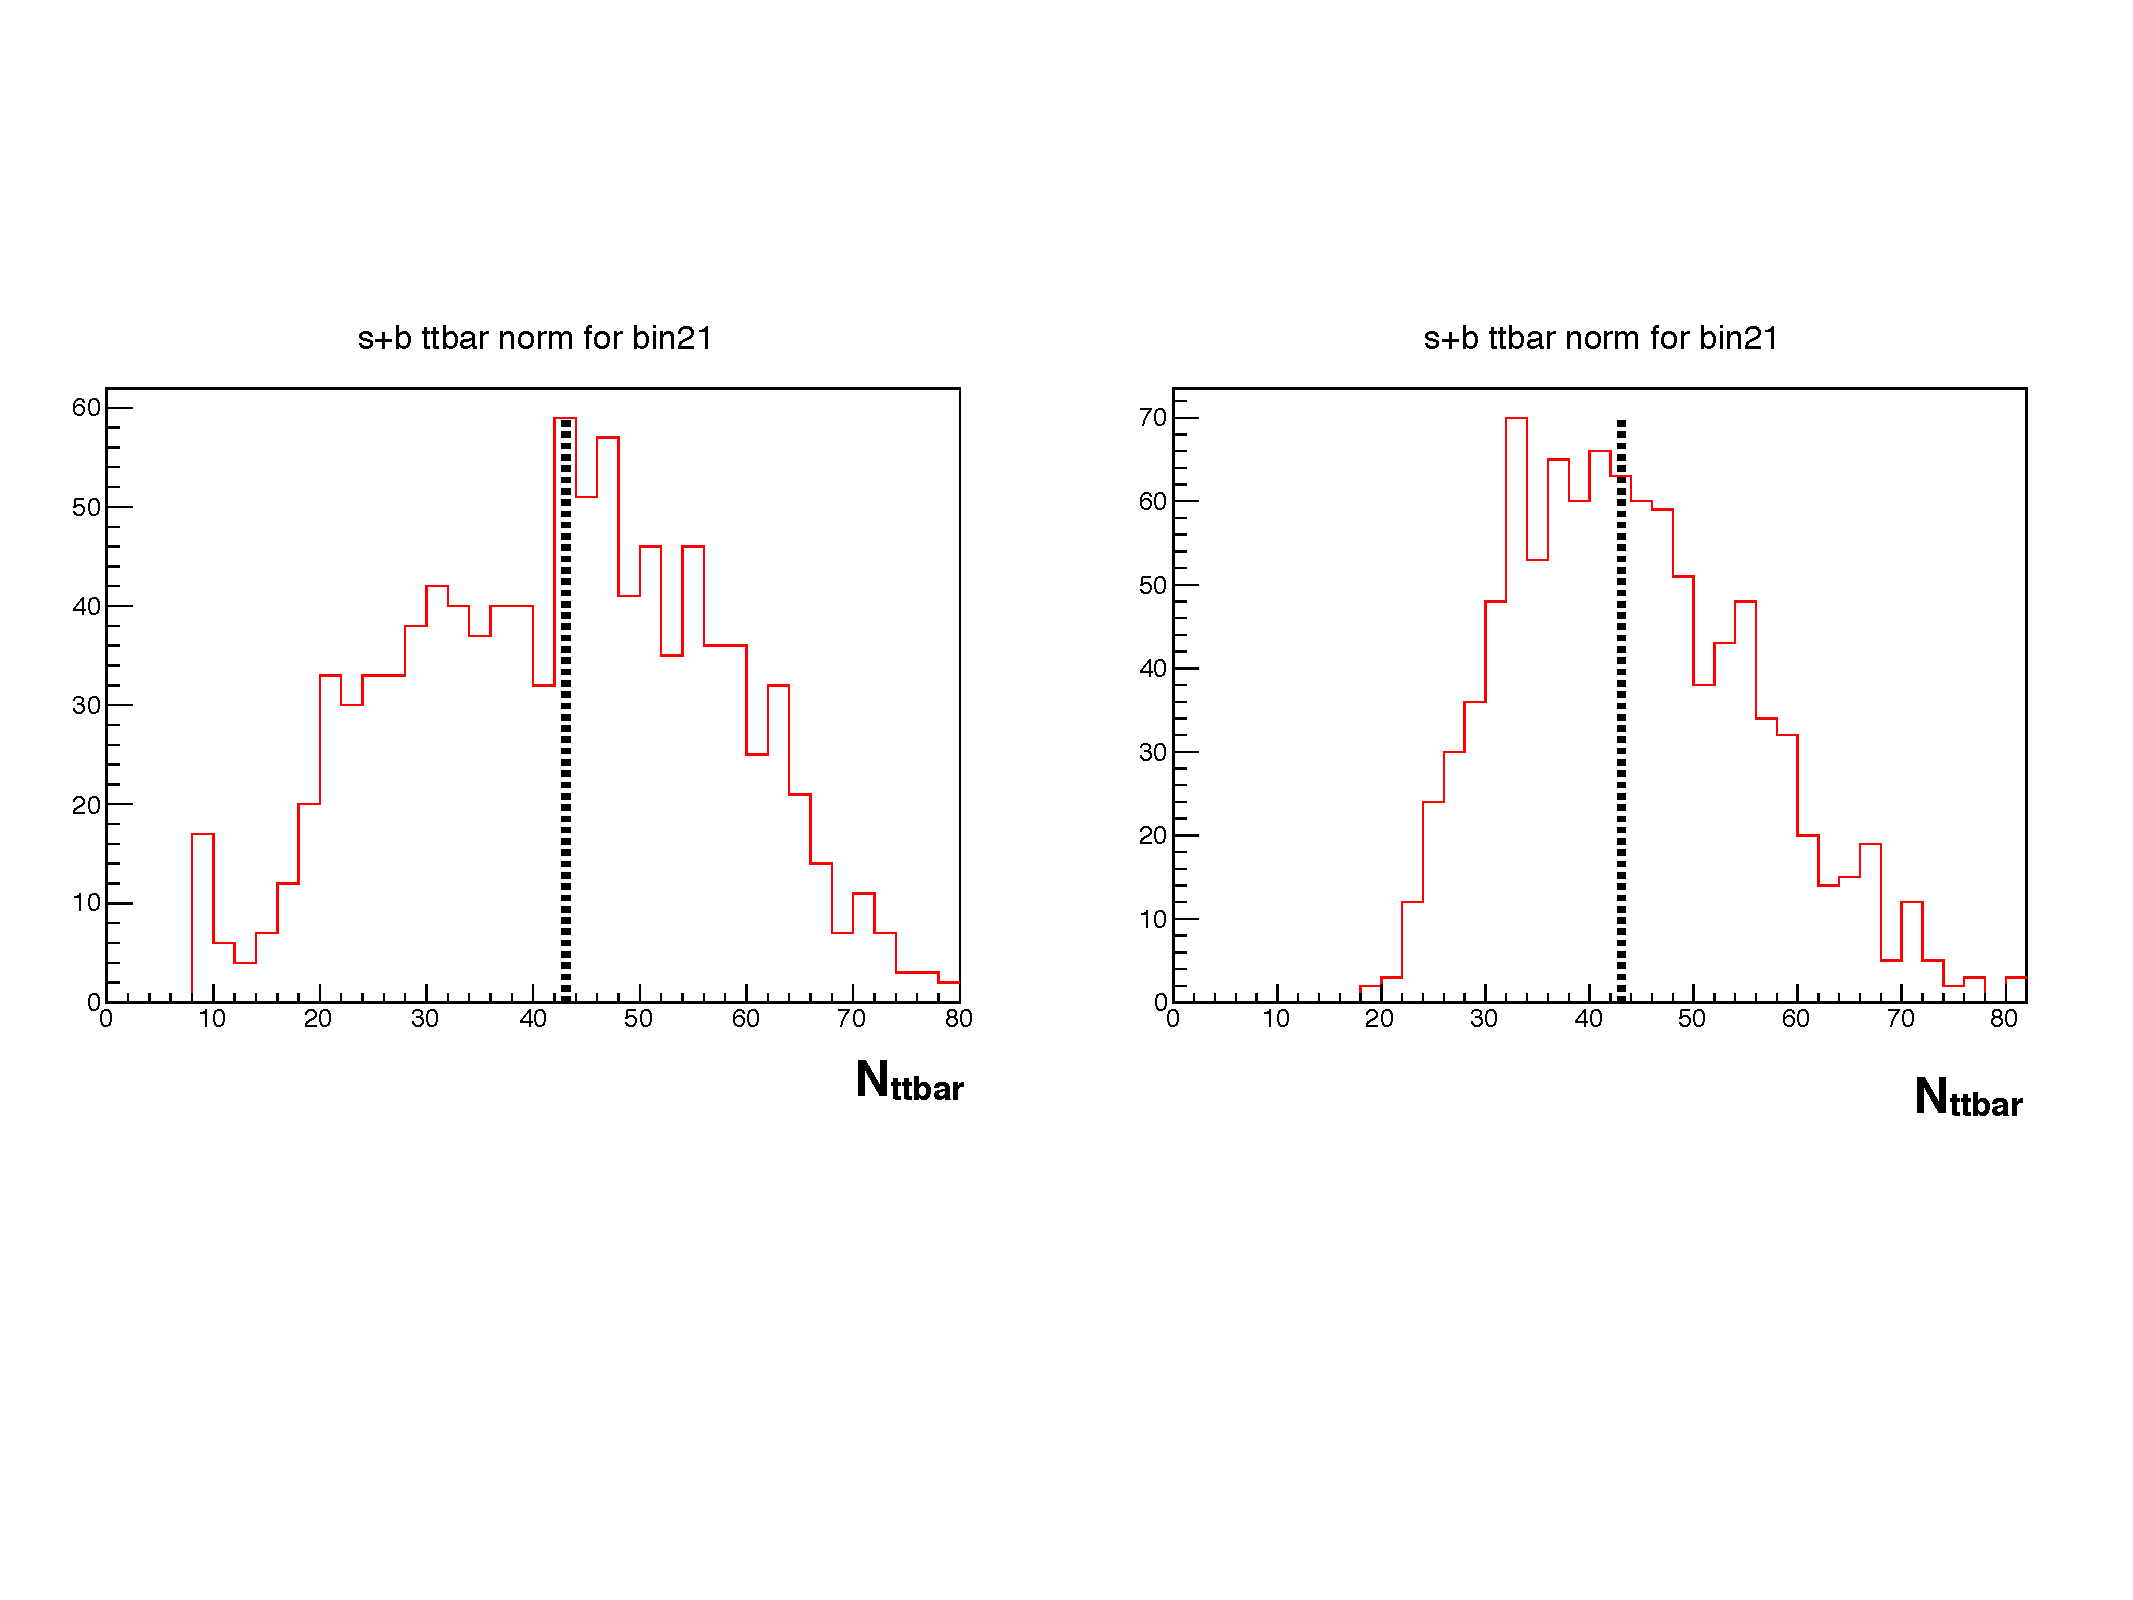
\includegraphics[angle=0,width=0.90\columnwidth]{fig/mj_connection_exps.pdf}
\caption{Distribution of post-fit yields of \ttbar in the $\Njets \geq 8$, $\MJ > 1000~\GeV$ bin for 1,000 psuedodata experiments without (left) and with (right) constraints between adjacent \MJ bins.
The dotted black line indicates the the pre-fit yield.}
\label{fig:mj_connection_exps}
\end{figure}

\begin{figure}[tbp!]
\centering
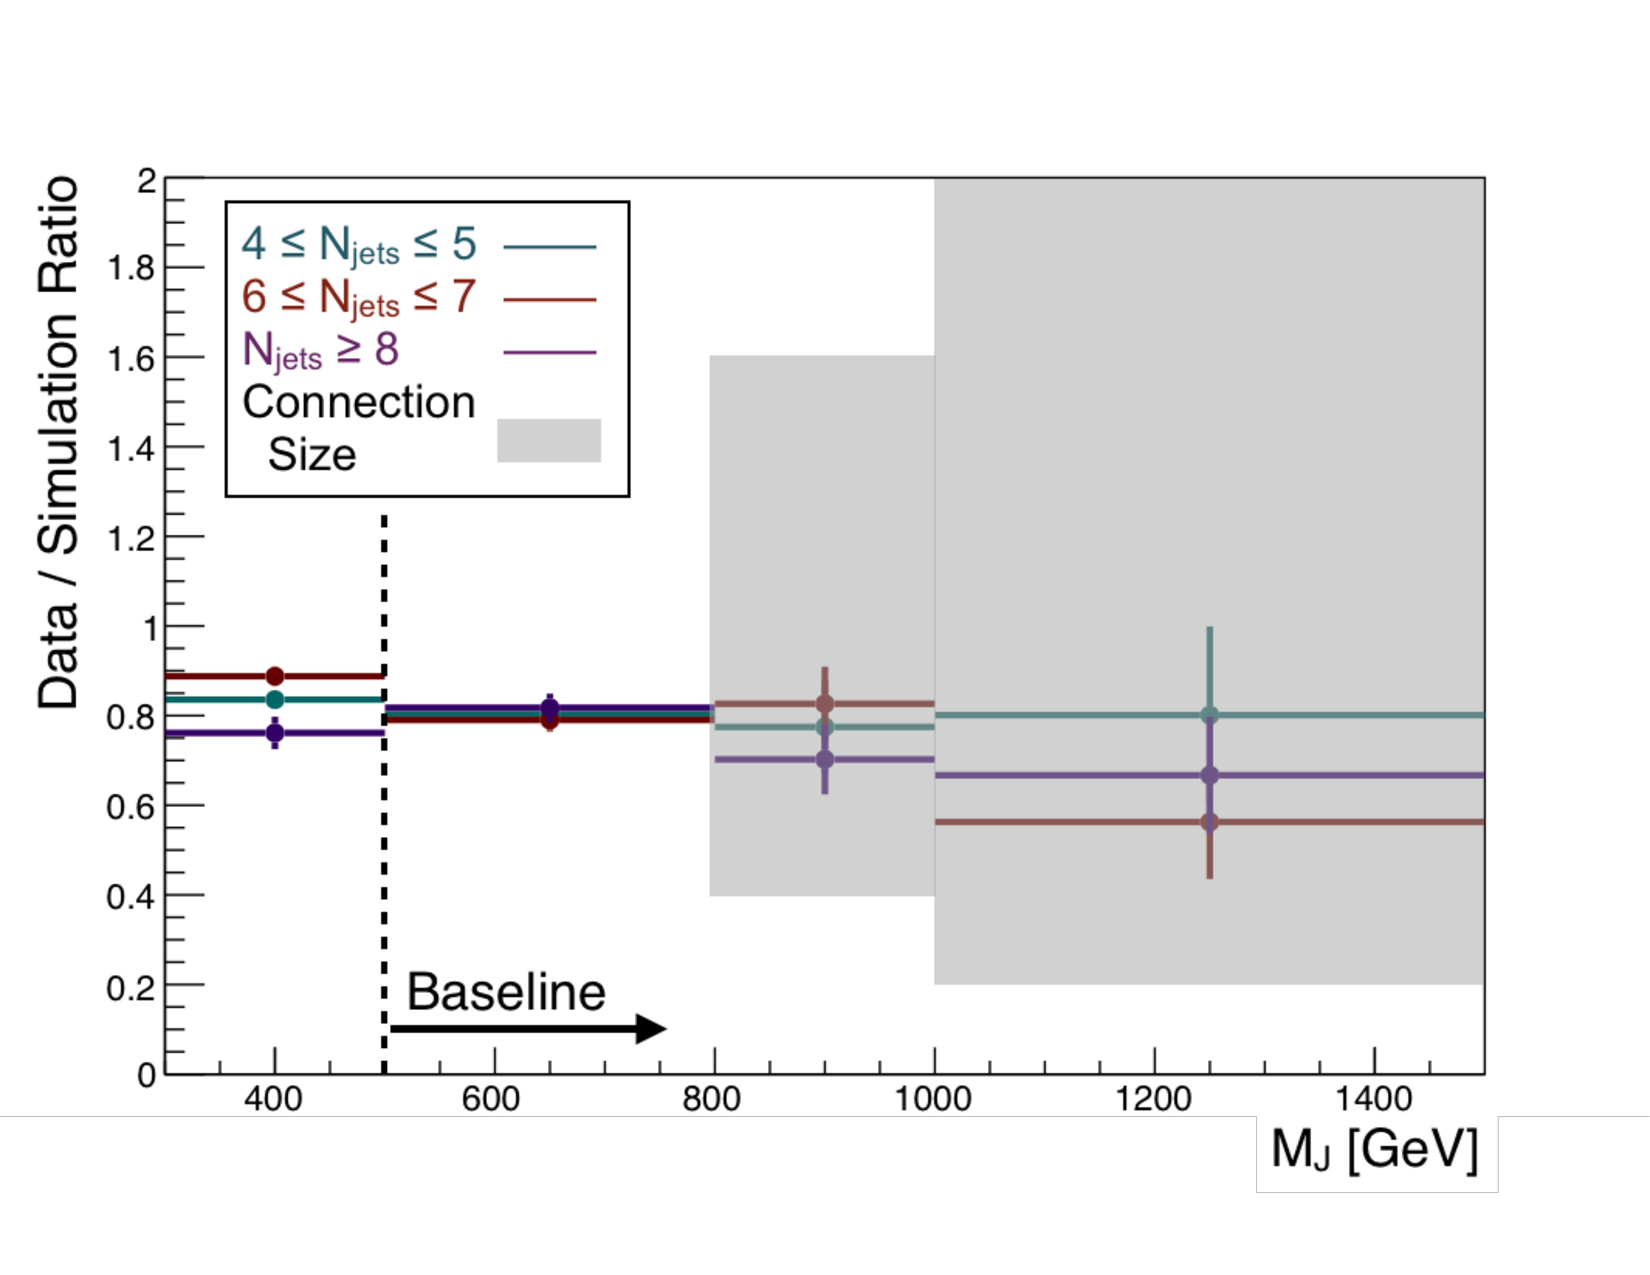
\includegraphics[angle=0,width=0.60\columnwidth]{fig/mj_connection.pdf}
\caption{Data-to-simulation ratios as a function of \MJ for different \Njets bins (data points) with a selection of $\Nleps = 1$, $\HT > 1200~\GeV$, and $\Nb = 1$ applied.
The shaded region corresponds to the size of the \MJ connection in each \MJ bin.}
\label{fig:mj_connection}
\end{figure}

\end{subsection}

\end{section}

\begin{section}{\Wjets Normalization}

The \Wjets background is determined in the fit with one global normalization parameter and two parameters to adjust the bin-to-bin normalization of adjacent \Njets bins, since the \Njets sahpe may not be well-modelled by simulation.
The amount the \Njets shape may vary is based on the data-to-simulation agreement in a kinematically similar \Zjets sample selected with $\Nleps = 2$ ($\mathrm{ee}$ or $\mu\mu$), $\HT > 1200~\GeV$, $\MJ > 500~\GeV$, $\Nb = 1$, and $80 < \mll < 100~\GeV$, where $\mll$ is the invariant mass of the two leptons.
The \Njets distribution and data/simulation yields ratio for this sample are shown in Figure~\ref{fig:njets_dy}.
The resulting variation sizes are 17\% between $4 \leq \Njets \leq 5$ and $6 \leq \Njets \leq 7$ and 62\% between $6 \le \Njets \le 7$ and $\Njets \ge8$.
After correcting the \Njets spectrum, the residual \MJ mismodeling is expected to be small, so no further correction is applied.

\begin{figure}[tbp!]
\centering
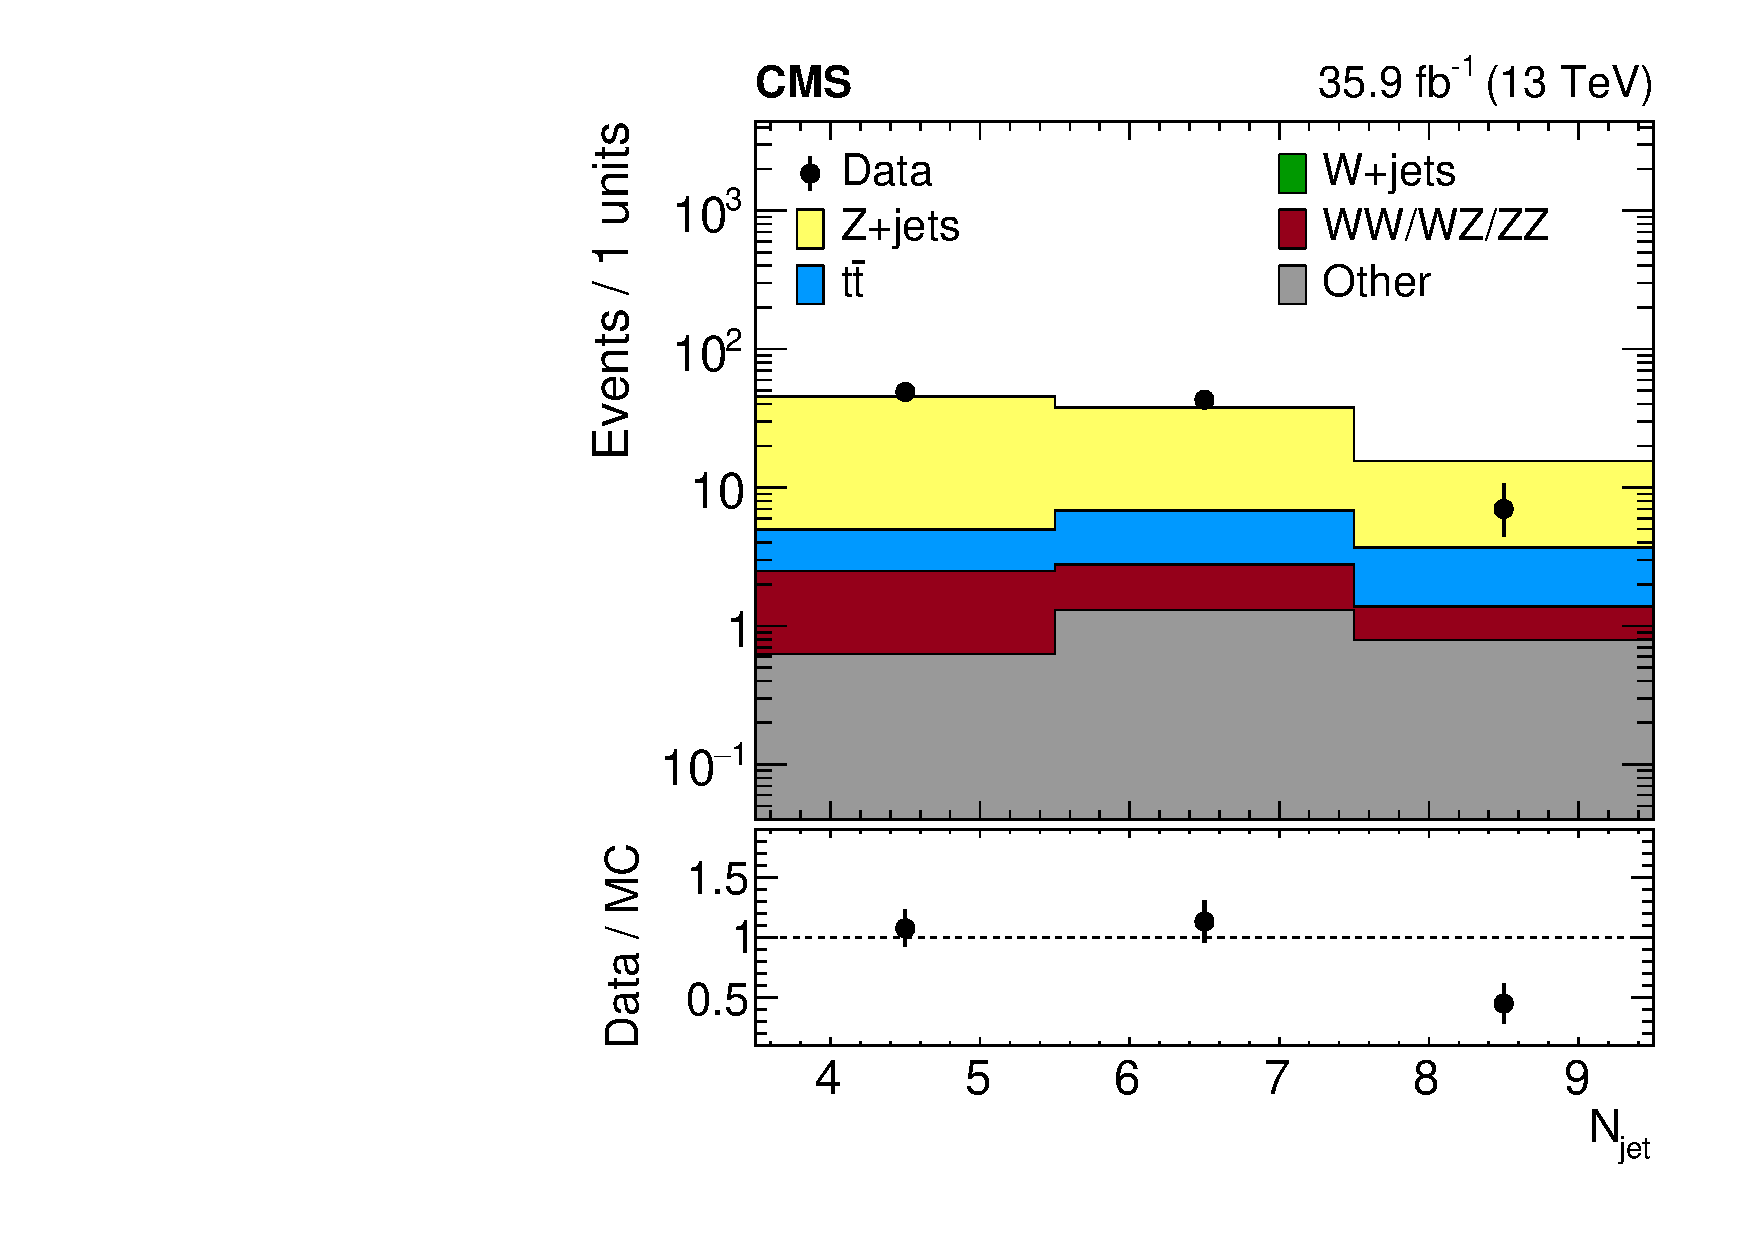
\includegraphics[angle=0,width=0.60\columnwidth]{fig/njets_dy.pdf}
\caption{Jet multiplicity distribution for data and simulation in a \Zjets control sample selected by requiring $\Nleps = 2$, $\HT > 1200~\GeV$, $\MJ > 500~\GeV$, $\Nb = 1$, and $80 < \mll < 100~\GeV$.
The total yield from simulation is normalized to the number of events in data.
The uncertainty in the ratio of data to simulation yields (lower panel) is statistical only.}
\label{fig:njets_dy}
\end{figure}

\end{section}

\begin{section}{Other Normalization}

The nominal normalization for Other is largely taken from simulation, as its contribution is less than 20\% in every bin with typical values $\lesssim 5\%$.
It is, however, allowed to vary according to statistical and systematic uncertainties.

\end{section}

\chapter{Systematic Uncertainties}

The nominal simulated shape of the \Nb distribution is allowed to vary by the inclusion of systematic uncertainties.
Each uncertainty is incorporated in the fit with template \Nb histograms to account for the effects of the systematic variation and a nuisance parameter $\theta$ to control the variation amplitude.
The nuisance parameters are subject to Gaussian constraints, normalized so that $\theta=0$ corresponds to the nominal \Nb shape and $\theta=\pm1$ corresponds to $\pm1$ standard deviation (s.d.)\ variation of the systematic uncertainty.
These uncertainties affect only the \Nb shape for \ttbar, QCD, and W+jets backgrounds, because their normalizations are determined from data, while for the other (subleading) backgrounds the uncertainties affect both the \Nb shape and normalization.

\begin{section}{Gluon Splitting Rate}

The primary source of systematic uncertainty is on the modelling of the rate of gluon splitting, as events with a gluon splitting to \bbbar provide an additional source of b quarks in events.
As this process may not be properly simulated, constraining the splitting rate in data is crucial for establishing a robust prediction of the \Nb distribution.
The dominant contribution of this effect is due to gluons that split specifically to b~quark pairs, so the phrase ``gluon splitting'' will hereafter refer exclusively to gluon splitting to \bbbar.
One way to select a data sample enriched in gluon splitting events is to use the \dRbb distribution, where \dRbb is defined as the $\Delta R$ between two b-tagged jets, as pairs of b-tagged jets resulting from the same gluon splitting tend to have smaller values of \dRbb than pairs resulting from hard scatter b-quarks or fakes.
This can be seen in Figure~\ref{fig:dRbb_shapes}, which shows the dRbb distribution in simulated QCD events with $\Nb = 2$ for three important categories:
Events that have a correlated pair of b-tagged jets originating from a gluon splitting (green, denoted GSbb) populate the low-\dRbb region, while events without gluon splitting (yellow, denoted noGS) or where the splitting yields zero one b-tagged jets (blue, denoted GSb) populate the low-and high-\dRbb regions roughly equally.

\begin{figure}[tbp!]
\begin{center}
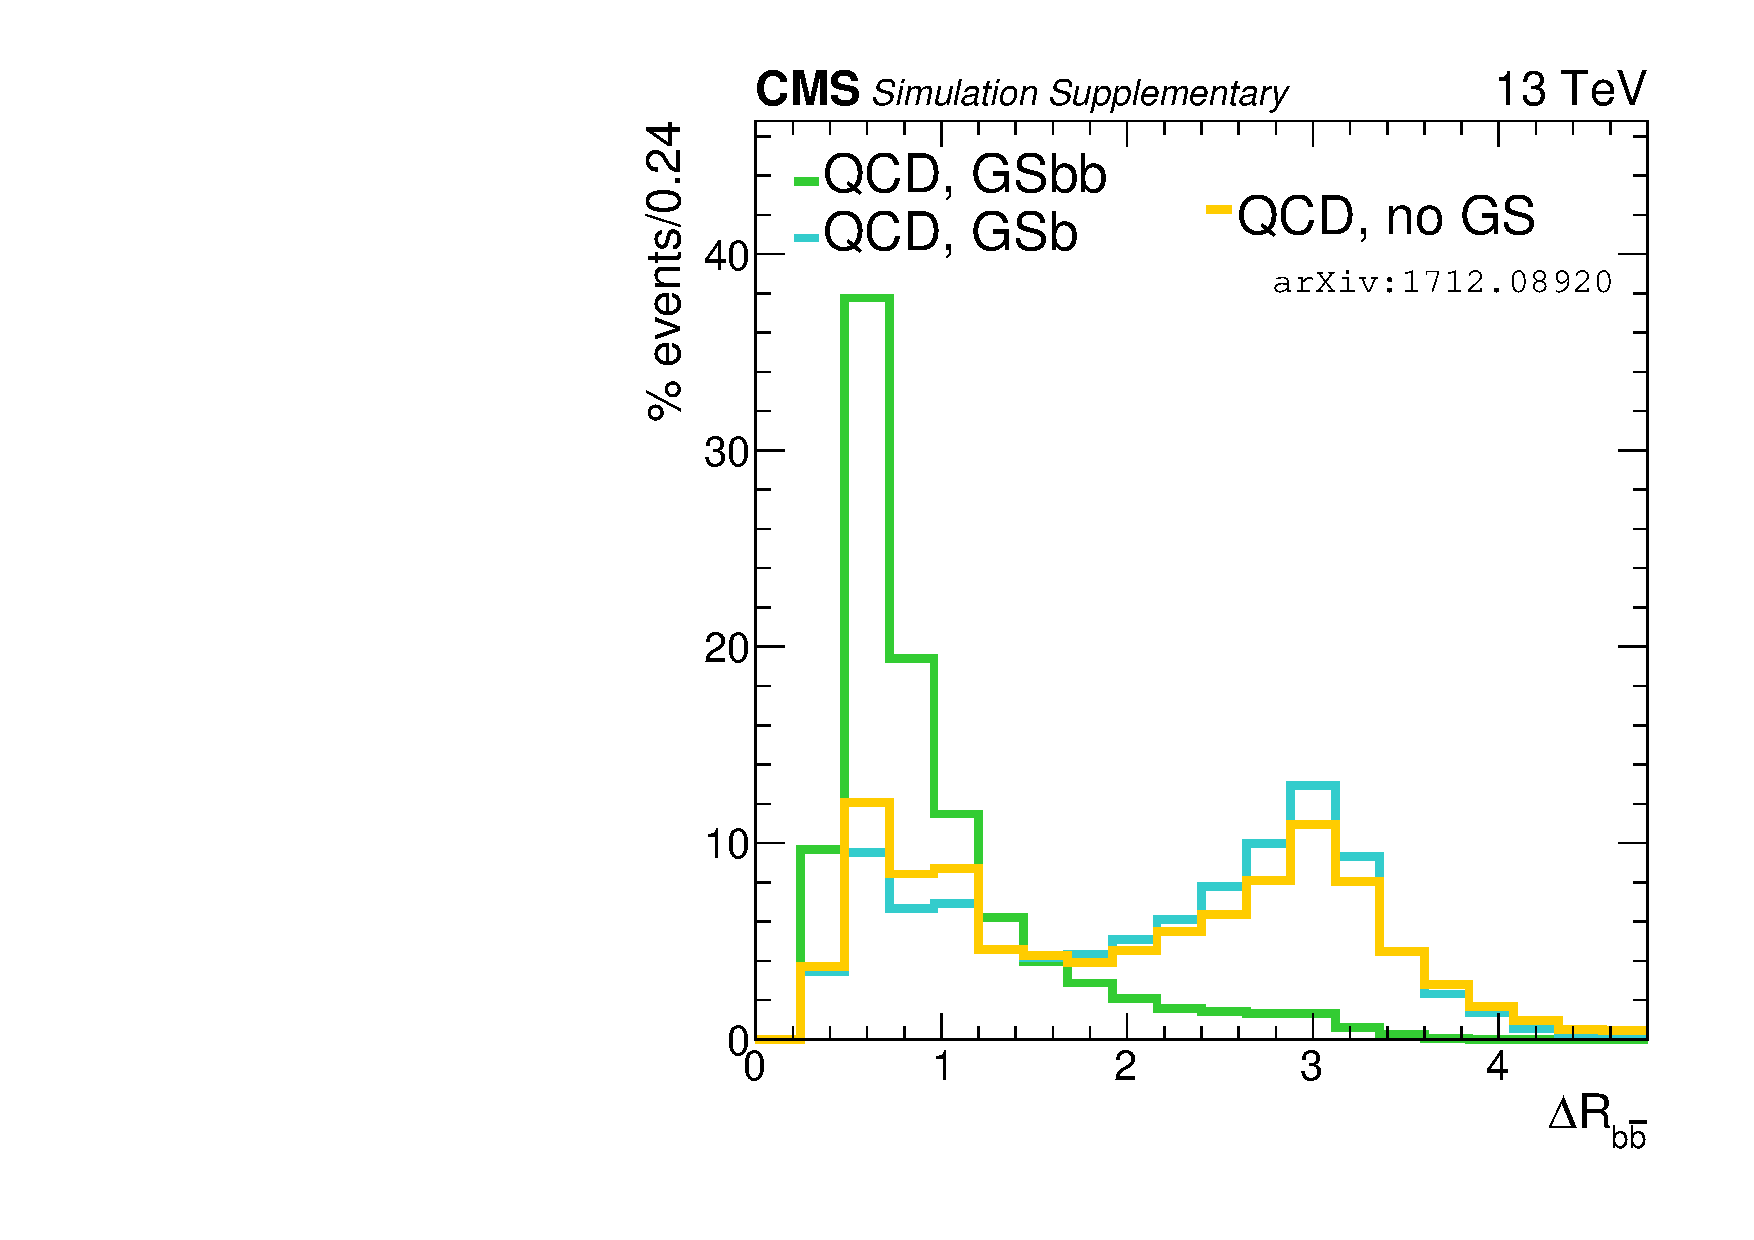
\includegraphics[angle=0,width=0.60\columnwidth]{fig/dRbb_shapes.pdf}
\end{center}
\caption{The \dRbb distribution shapes for the three gluon splitting categories: 
Events with a pair of b-tagged jets resulting from gluon splitting (green), events with a gluon splitting yielding fewer than 2 b-tagged jets (blue), and events without a gluon splitting to \bbbar.
These events are selected by requiring $\Nleps = 0$, $\HT > 1500~\GeV$, $\MJ > 500~\GeV$, $\Njets \geq 4$, and $\Nb = 2$.}
\label{fig:dRbb_shapes}
\end{figure}

Gluon splittings can contribute less than 2 b-tagged jets either because the quarks are collimated into a single jet, one of the b-tagged jets is not tagged, or because one of the jets fails to pass the jet selection criteria, typically because it is too soft.
The relative fractions of these contributions is shown in Figure~\ref{fig:gs_categories}.

\begin{figure}[tbp!]
\begin{center}
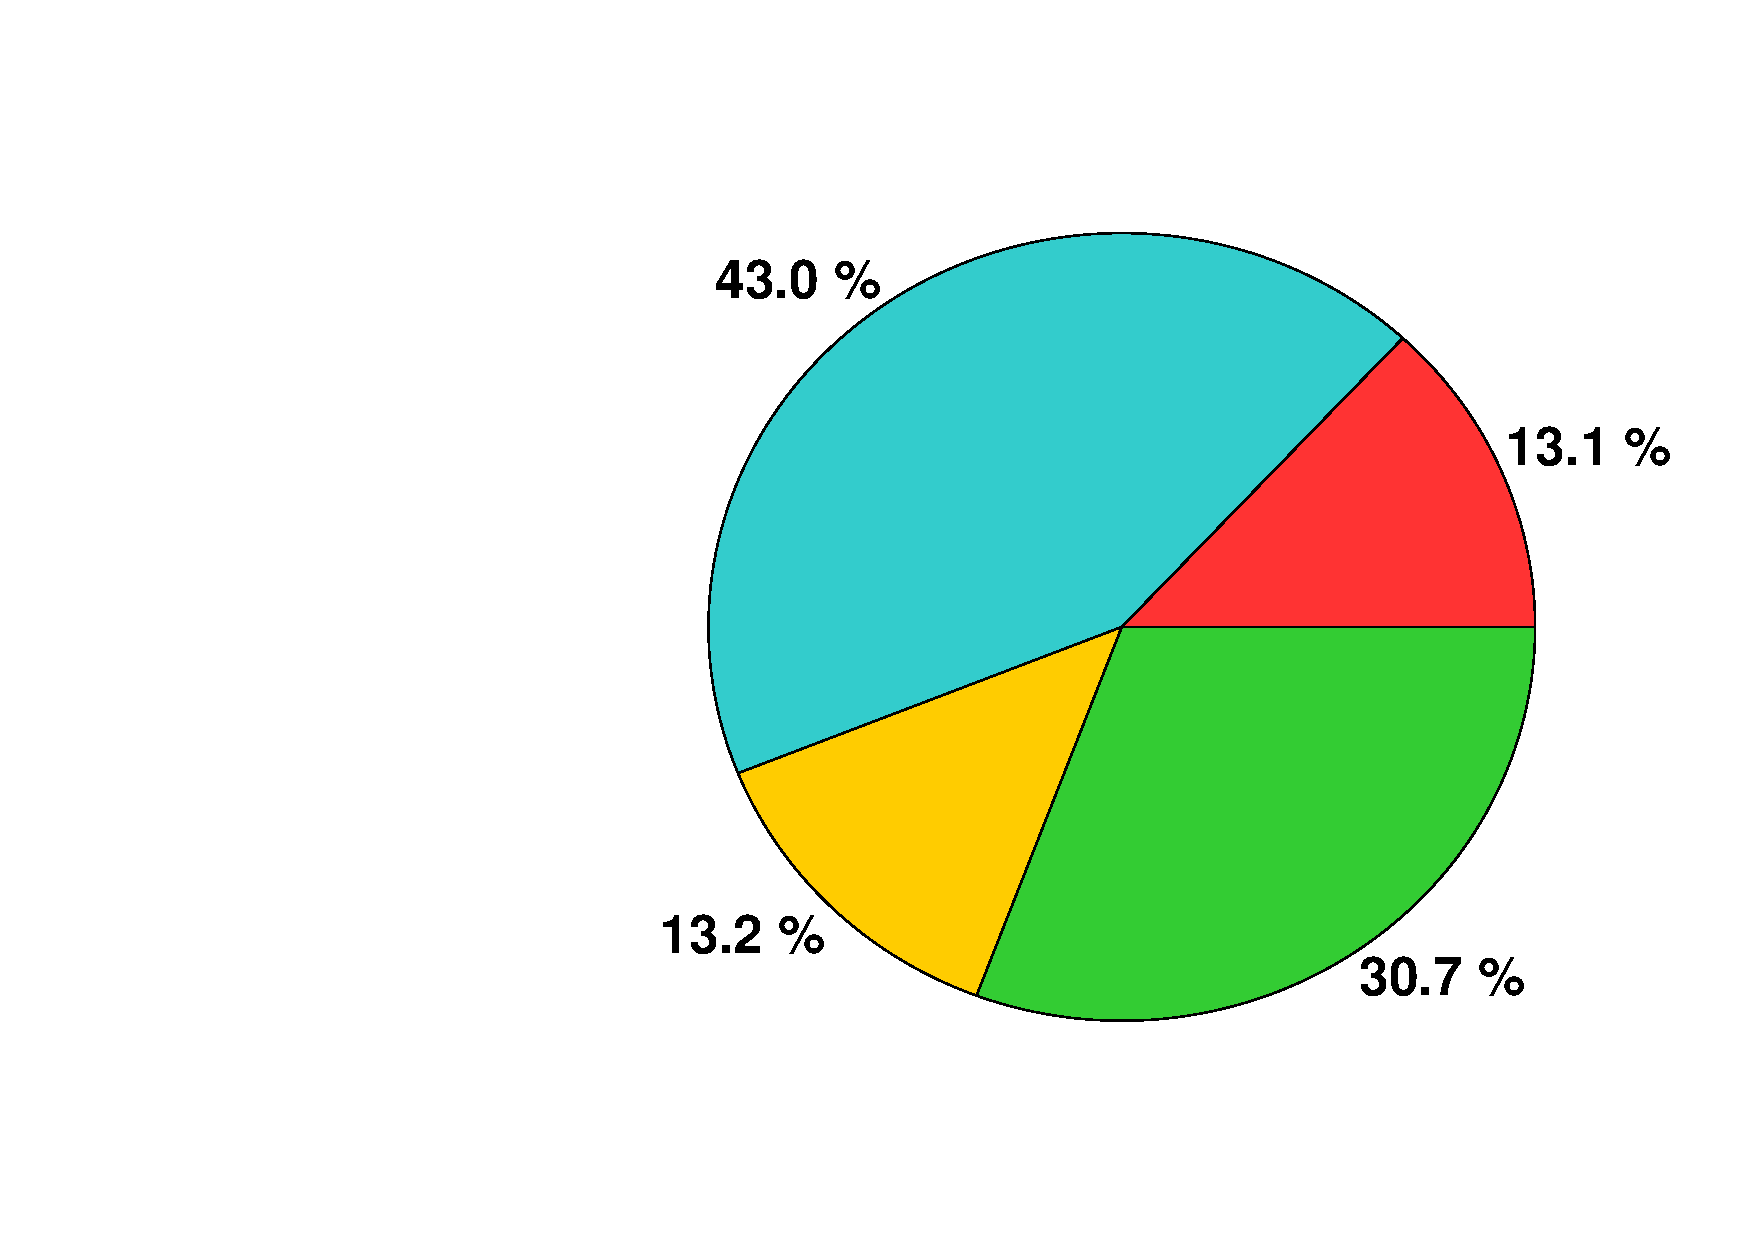
\includegraphics[angle=0,width=0.45\columnwidth]{fig/gs_piechart.pdf}
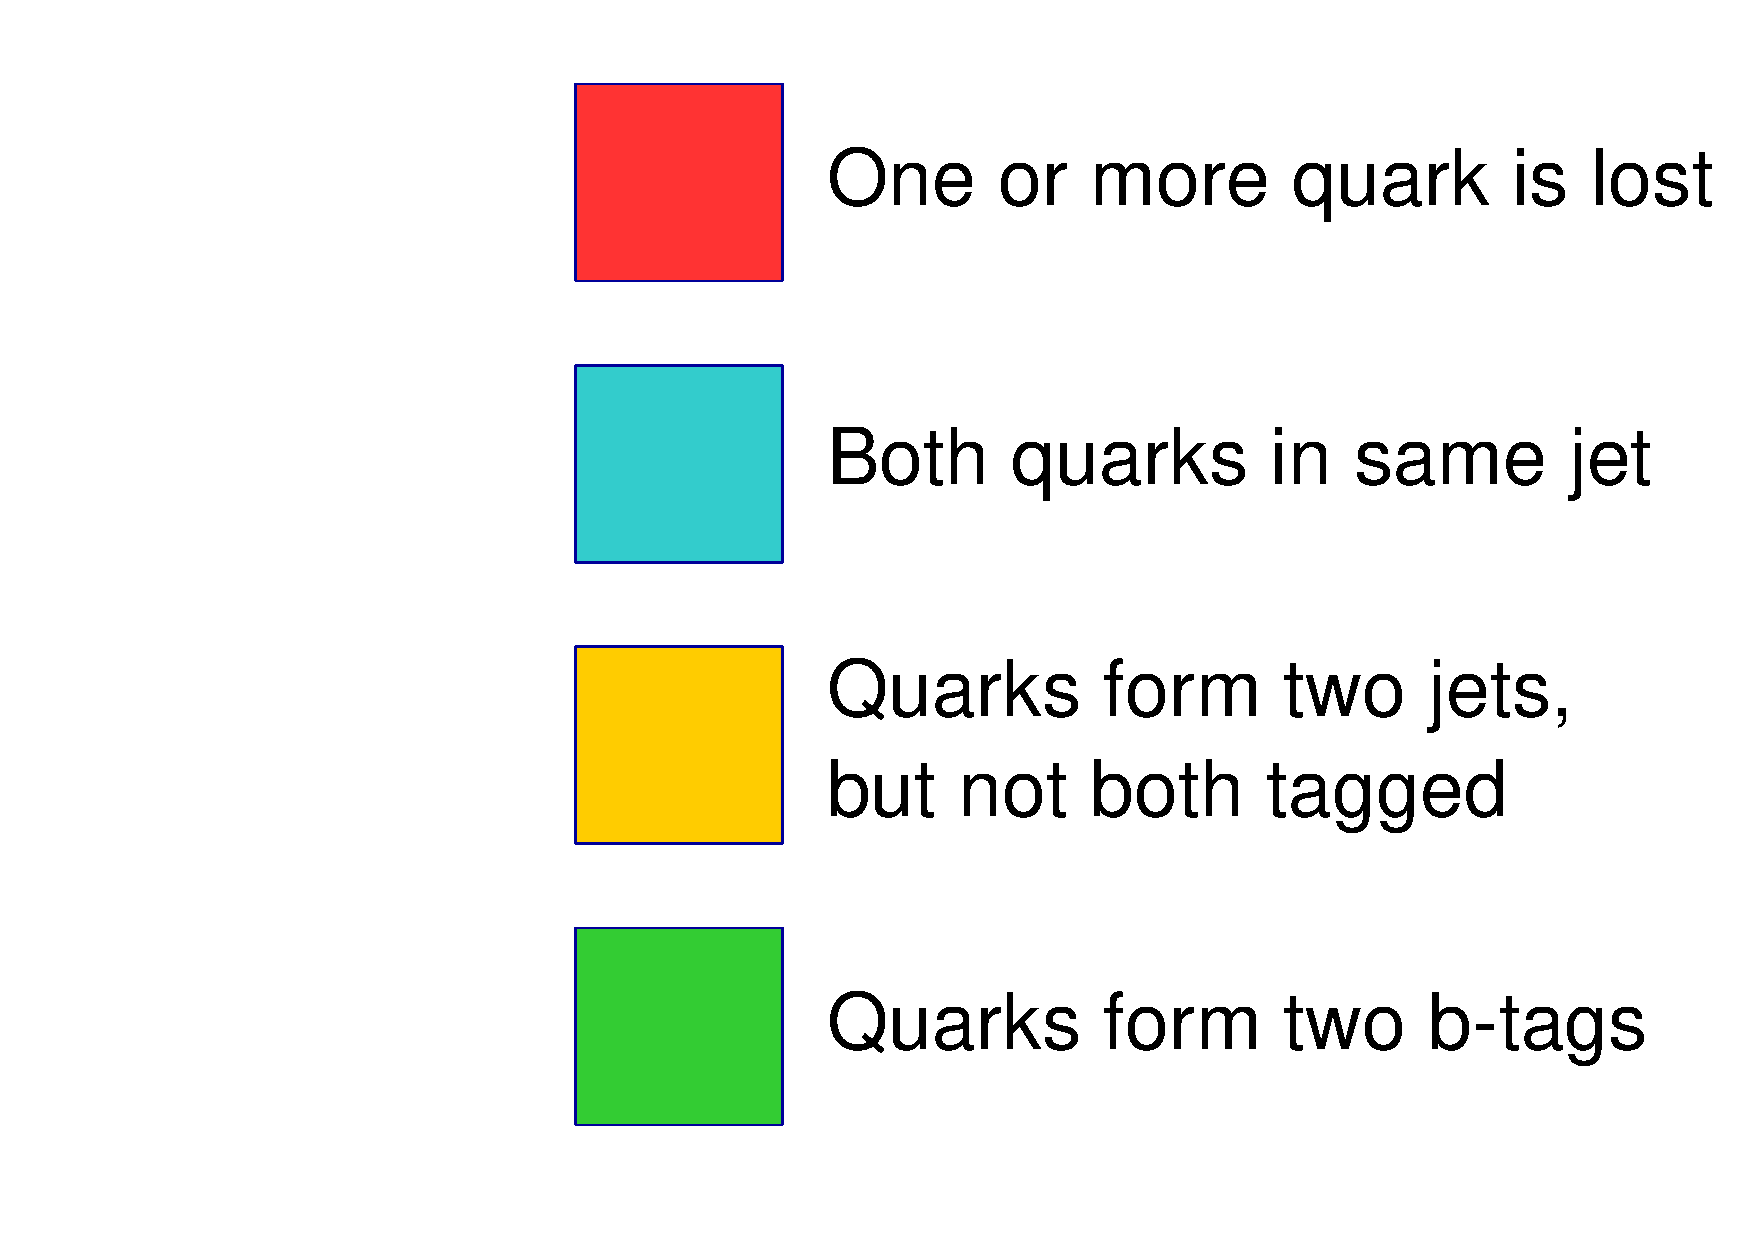
\includegraphics[angle=0,width=0.45\columnwidth]{fig/gs_piechart_legend.pdf}
\end{center}
\caption{The relative fraction of the possible final states that occur from gluon splitting to \bbbar for events satisfying $\Nleps = 0$, $\HT > 1500~\GeV$, $\MJ > 500~\GeV$, $\Njets \geq 4$, and $\Nb = 2$.}
\label{fig:gs_categories}
\end{figure}

The gluon splitting rate is the constrained by fitting the \dRbb distribution by using the difference in shapes of the GSbb, GSb, and noGS categories.
This fit varies the normalization of the GSbb and GSb (varied together) and the noGS contributions in order to extract the relative contributions of events with and without a gluon splitting.
It is performed in four equal bins in the range of $0 \leq \dRbb < 4.8$ with events selected by requiring $\Nleps = 0$, $\HT > 1500\GeV$, $\Nb = 2$, $\Njets \geq 4$, and $\MJ > 500~\GeV$ as the gluon splitting signal in a $\Nleps = 1$ control sample is contaminated by b~quarks from the decay of top quarks.
Additionally, the $\Nleps = 0$ control sample is formed from a subset of the data that is selected to be most stable in the b~tagging algorithm performance, since the precision of the \dRbb fit is not limited by the data sample size.
This choice isolates the physical effects of gluon splitting from the potential time dependence of the b~tagging performance due to variations in experimental conditions, which are separately incorporated by the b-tag scale factor uncertainties.
% WHY NLEPS=0 region also works for NLEPS=1

The \dRbb fit extracts a weight of $0.77 \pm 0.09$ for gluon splitting events and a weight of $1.21 \pm 0.08$ for non-gluon splitting events.
The post-fit distributions are shown in Figure~\ref{fig:gs_fitresult}.
The GSbb and GSb categories are plotted separately to demonstrate the difference in shapes.
The discrepancy in the last bin does not significantly impact the fit because the higher yield bins at lower values of \dRbb constrain the fit.
The deviations of these weights from unity, summed in quadrature with their post-fit uncertainty, are used to form the $\pm 1$~s.d.\ variations of the gluon splitting rate nuisance parameter by applying weights of $1 \pm 0.25$ to gluon splitting events and $1 \mp 0.22$ to non-gluon splitting events in an anti-correlated manner.
The fit results are used as a measure of the uncertainty on modelling of the GS rate as opposed to a correction to the central value, since the \dRbb  variable may not be a perfect proxy for the GS rate.
Figure~\ref{fig:gs_variations} shows the effect of the $\pm 1$~s.d.\ variations on the \Nb distribution of \ttbar for the two most sensitive bins.

\begin{figure}[tbp!]
\begin{center}
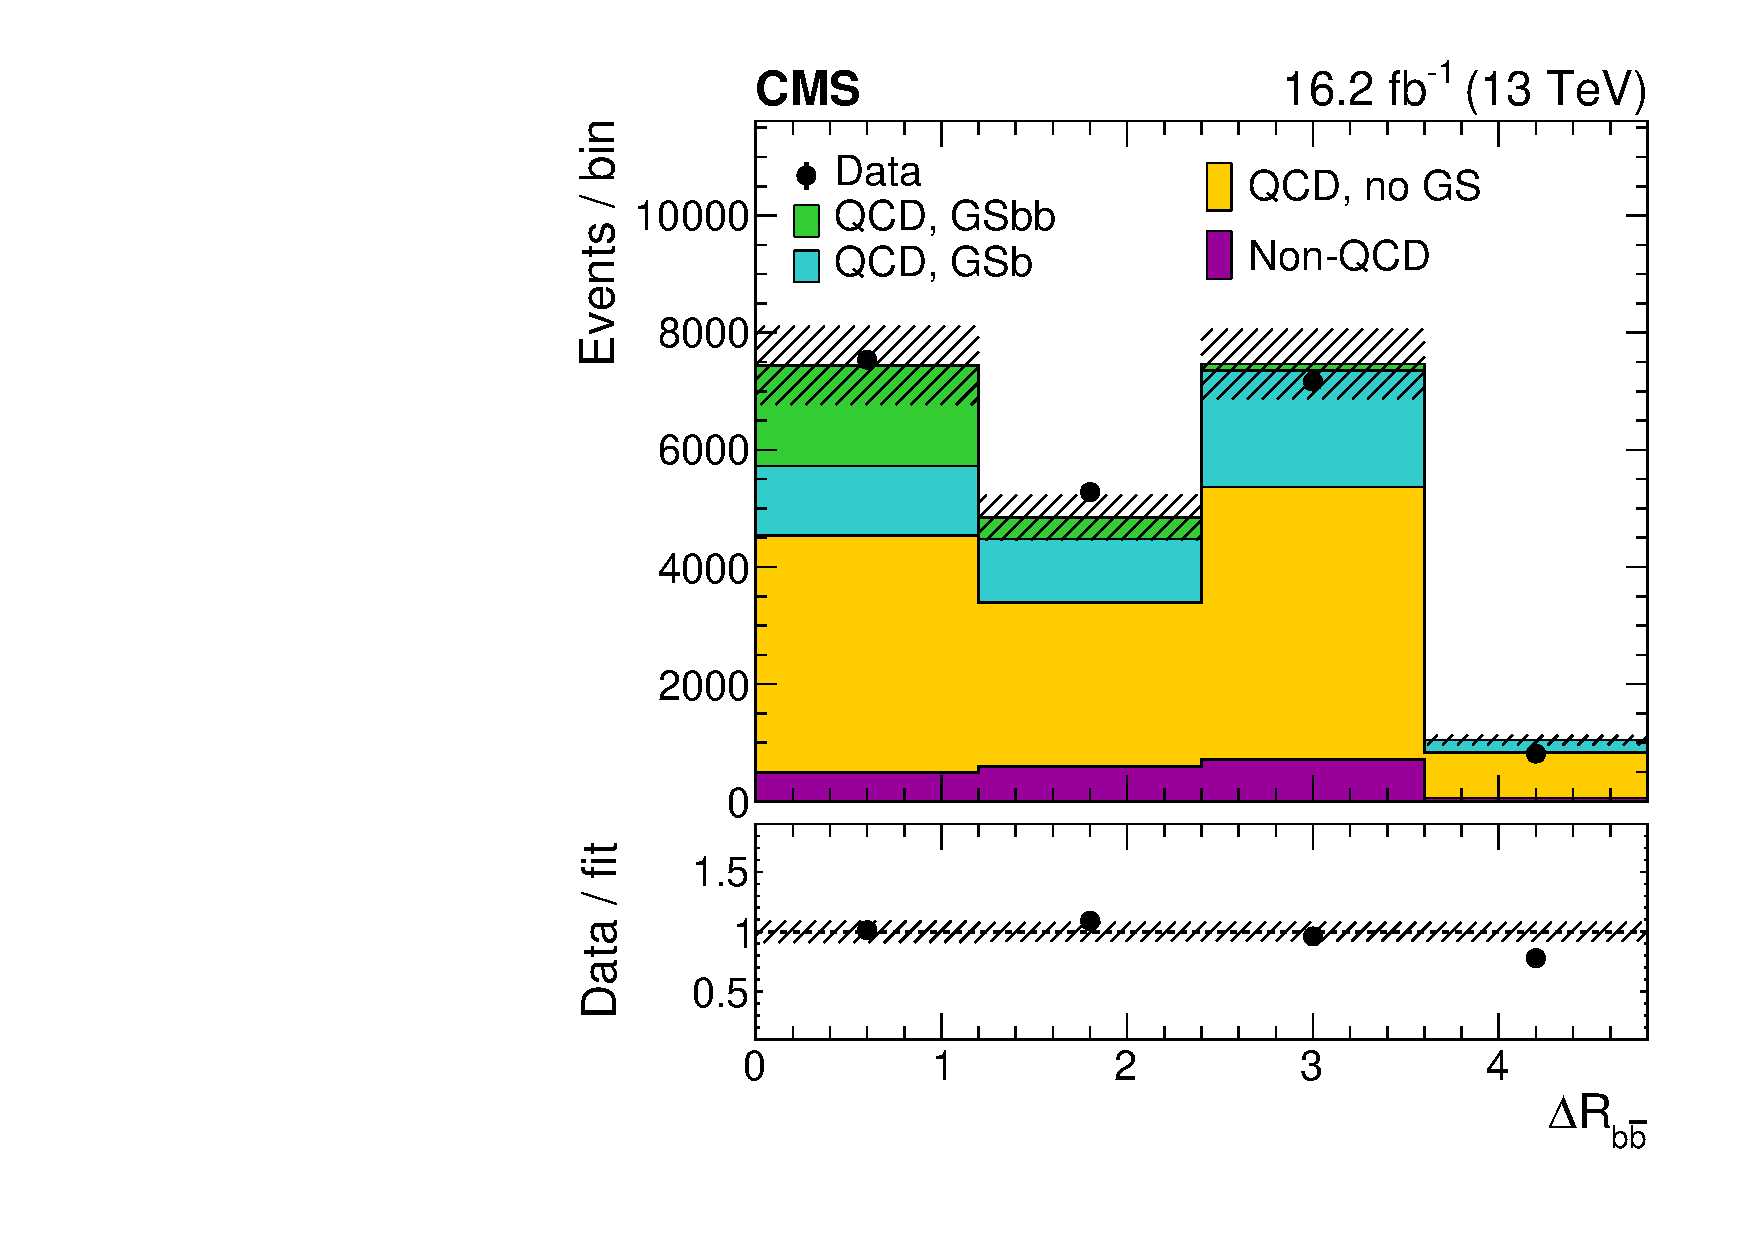
\includegraphics[angle=0,width=0.60\columnwidth]{fig/gs_fitresult.pdf}
\end{center}
\caption{Post-fit \dRbb distributions in a selection with  $\Nleps = 0$, $\HT > 1500~\GeV$, $\MJ > 500~\GeV$, $\Njets \geq 4$, and $\Nb = 2$ with the post-fit uncertainty represented by a hatched band.
The ratio of data to simulation yields is shown in the lower panel.}
\label{fig:gs_fitresult}
\end{figure}

\begin{figure}[tbp!]
\begin{center}
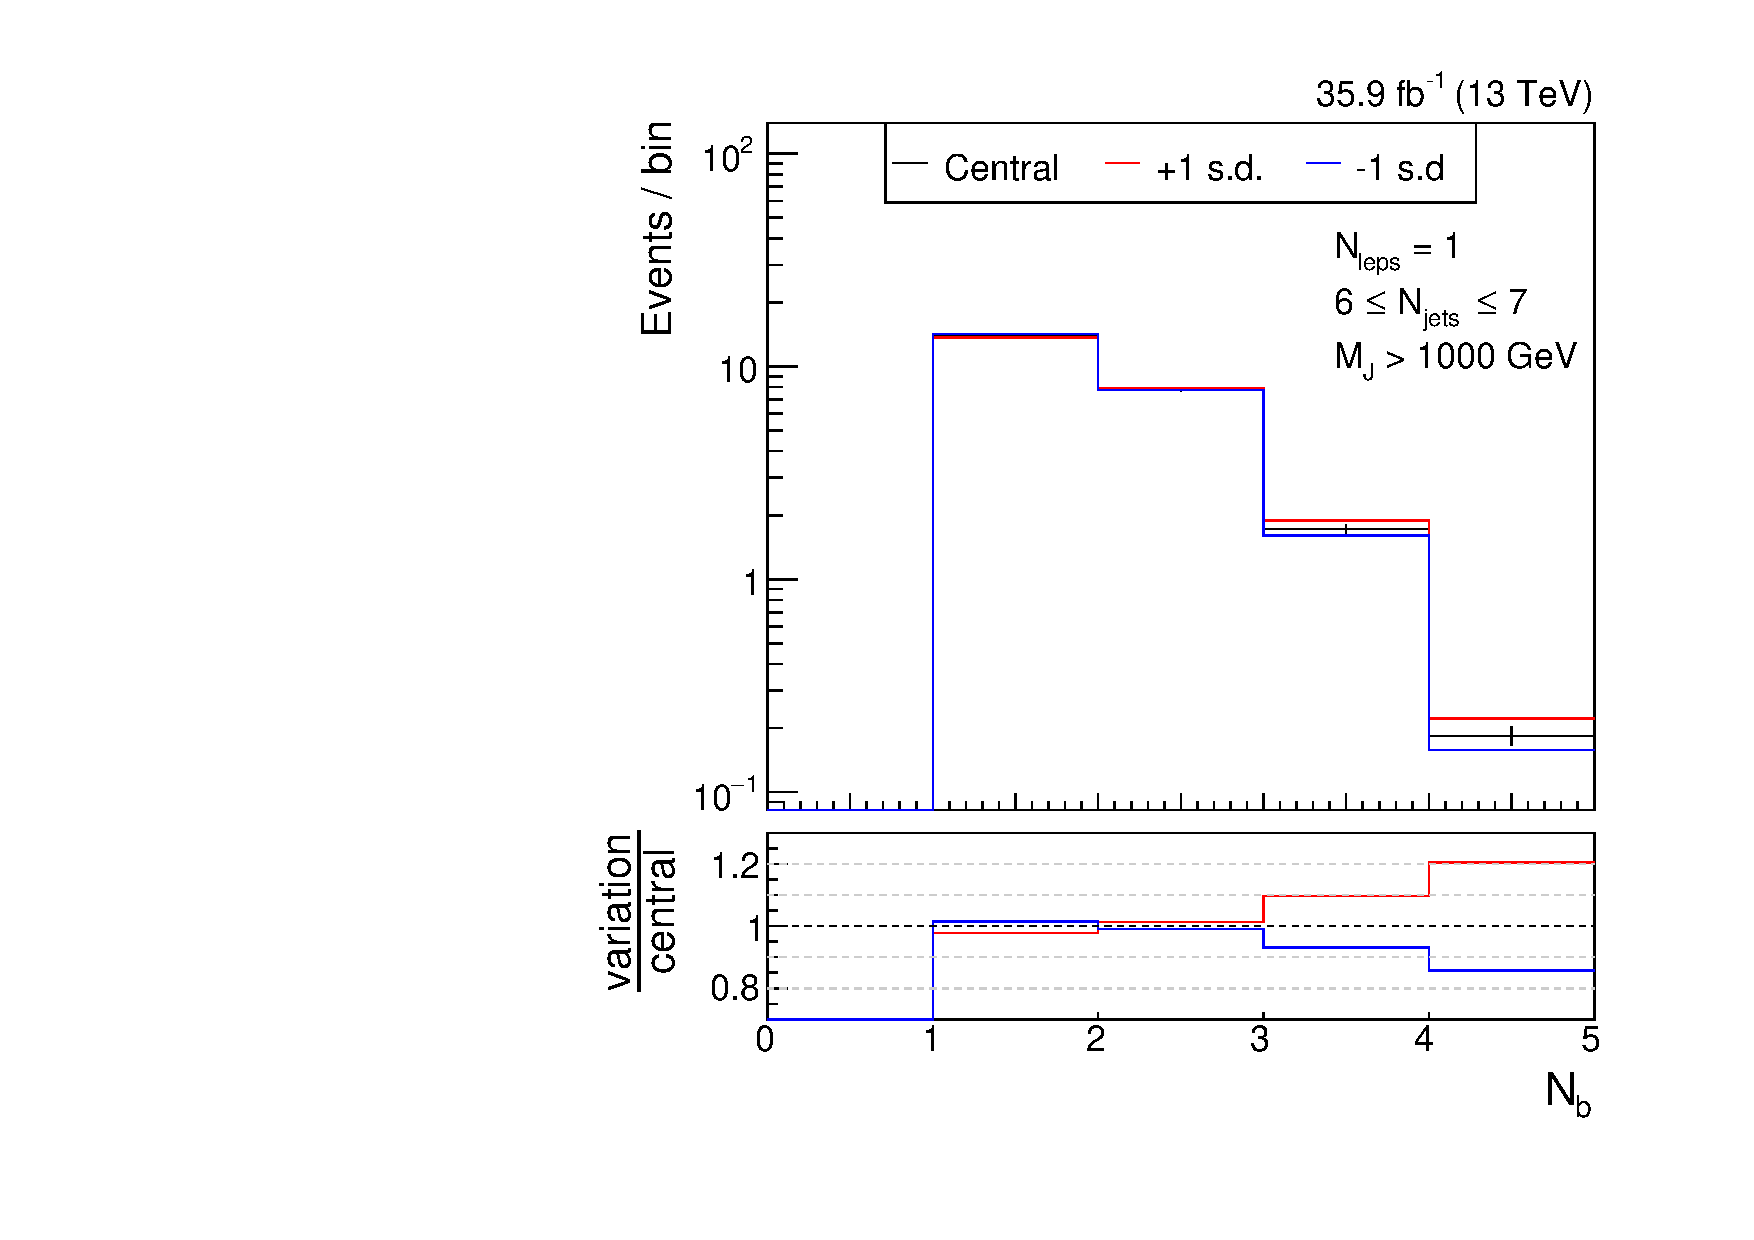
\includegraphics[angle=0,width=0.45\columnwidth]{fig/bin20_ttbar_gs_mconly.pdf}
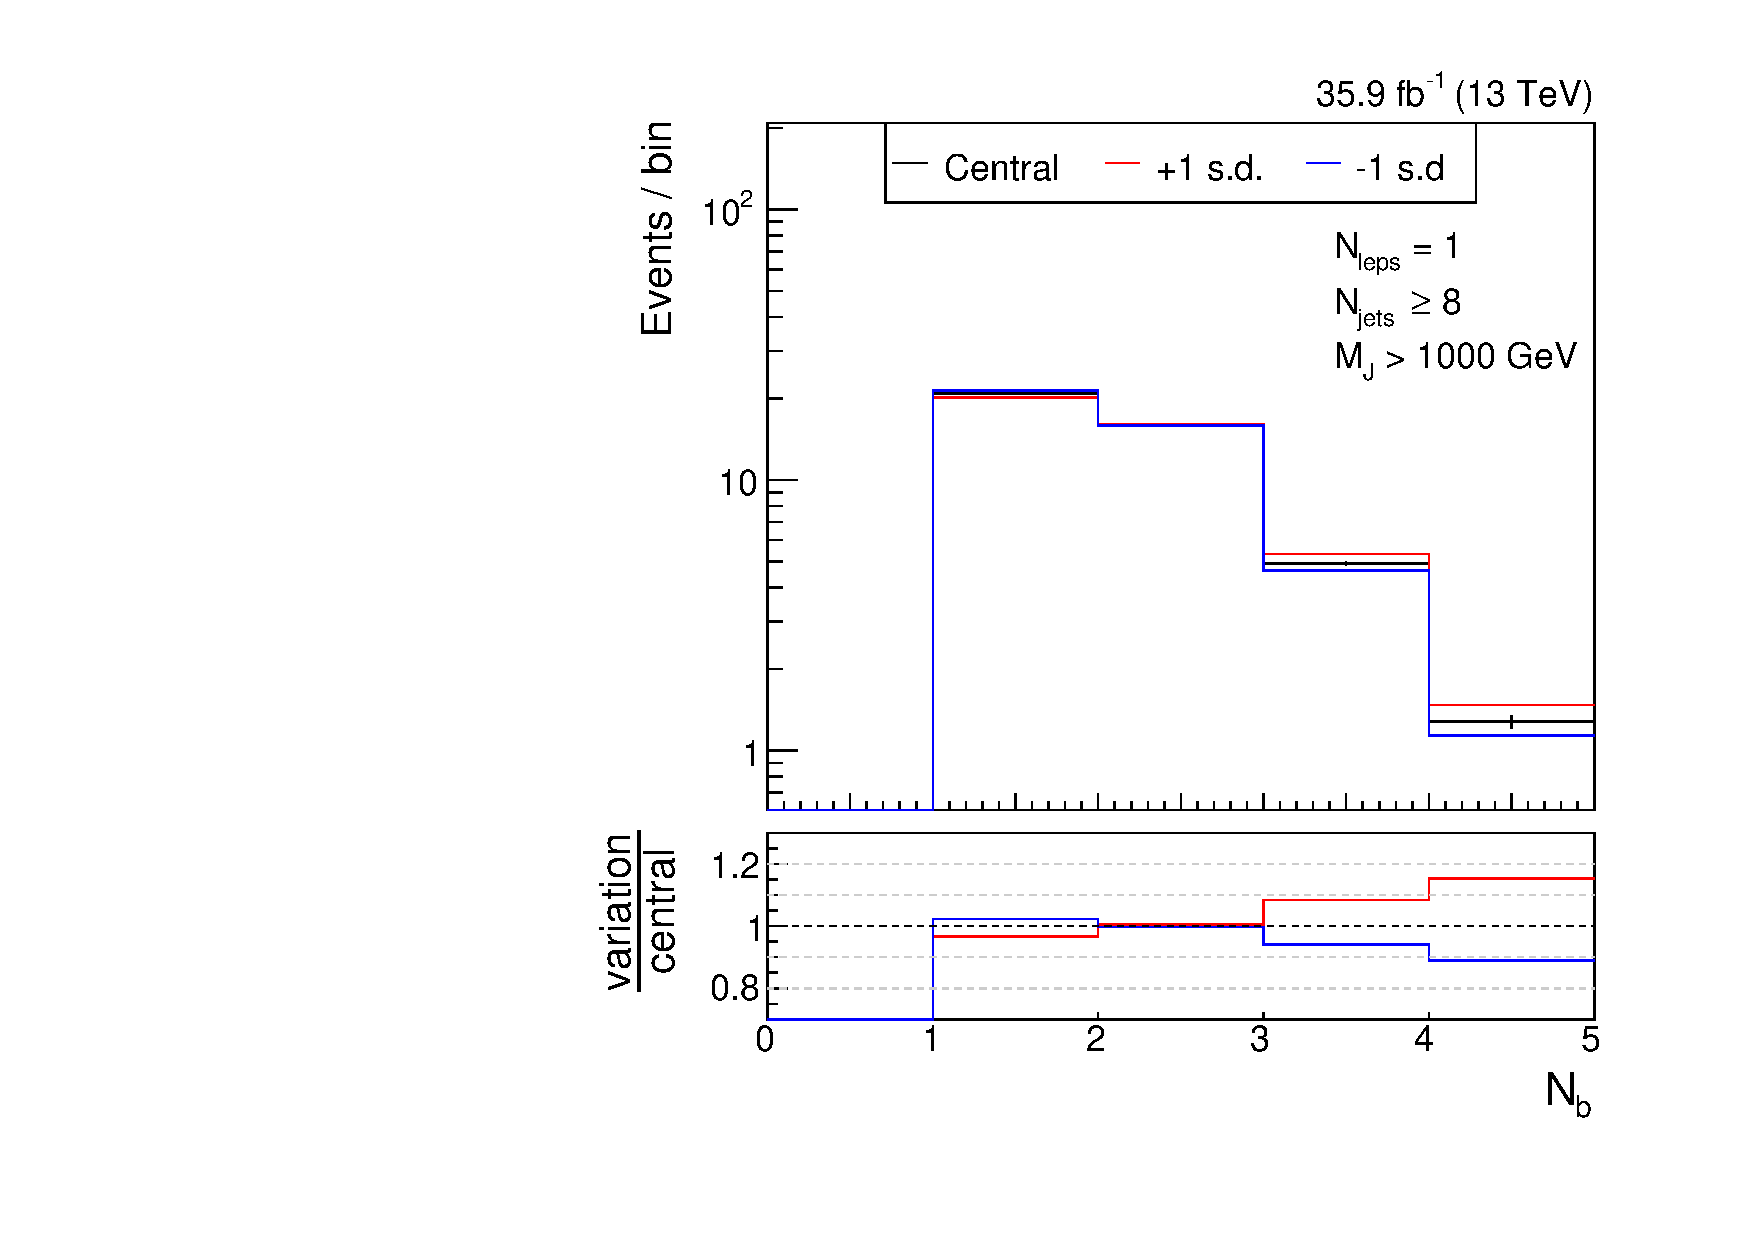
\includegraphics[angle=0,width=0.45\columnwidth]{fig/bin21_ttbar_gs_mconly.pdf}
\end{center}
\caption{Effect of the $\pm 1$~s.d.\ variations of the gluon splitting rate on the \Nb distribution in \ttbar events for the two most sensitive bins: ($\Njets \geq 8$, $800 < \MJ \leq 1000~\GeV$) (left) and ($\Njets \geq 8$, $\MJ > 1000~\GeV$) (right).
Event yields are normalized to that expected in $35.9~\ifb$ of data.}
\label{fig:gs_variations}
\end{figure}

In order to test the stability of the fit results and the dependence of the gluon splitting weights across kinematic regions, the \dRbb fit is repeated both with a higher \MJ threshold and with different \Njets bins. 
The resulting weights are shwon in Table~\ref{tab:gs_kinematic_bins} and are all consistent with those of the nominal fit.

\begin{table}[tb!]
\setlength\tabcolsep{3pt}
\centering
\begin{tabular}{l|cccccc}
 & Nominal & $\MJ > 800~\GeV$ & $4 \leq \Njets \leq 5$ & $6 \leq \Njets \leq 7$ & $8 \leq \Njets \leq 9$ & $\Njets \geq 10$ \\
\hline
GS    & $0.77 \pm 0.09$ & $0.70 \pm 0.38$ & $ 0.80 \pm 0.32$  & $ 0.76 \pm 0.14$ & $ 0.75 \pm 0.16$  & $ 0.95 \pm 0.36$ \\
No GS & $1.21 \pm 0.08$ & $1.28 \pm 0.35$ & $ 1.15 \pm 0.26$  & $ 1.22 \pm 0.13$ & $ 1.24 \pm 0.15$  & $ 1.05 \pm 0.36$ \\
\end{tabular}
\caption{Gluon splitting weights derived in the nominal fit, a variation with a requirement of $\MJ > 800~\GeV$, and 4 variations in bins of \Njets (with the nominal $\MJ > 500~\GeV$ requirement.)}
\label{tab:GS_variations}
\end{table}

\end{section}

\begin{section}{b-tagging Data-to-simulation Scale Factors}

Another significant systematic uncertainty is the uncertainty in the data-to-simulation scale factors (SF) for b~tagging efficiency and mistag rates.
Simulating the b-tagging algorithm relies on understanding the detailed behavior of the detector and also accurate modelling of the parton shower and hadronization, both of which are non-trivial.
Therefore, it is important to to measure the b~tagging efficiencies and mistag rates in data and correct the simulation to match.

The difference between data and simulation is corrected for by using a per jet data-to-simulation SF
\begin{align}
SF_{f} = \varepsilon^{data}_{f}(\pT)/\varepsilon^{sim.}_{f}(\pT).
\end{align}
where $\varepsilon^{data}_{f}(\pT)$ and $\varepsilon^{sim.}_{f}(\pT)$ are the tagging efficiencies for for a jet with flavor $f$ as a function of \pT in data and simulation, respectively.
No dependence on $\eta$ is derived due to limited data sample sizes.
In simulation, the efficiency is determined by matching jets to their generated hadron to determine their flavor and then measuring how many of those jets are correctly tagged.
In data, this is done by using control regions determined by specific selection requirements that produce pure samples of a certain flavor of jets while not biasing the jets with respect to variables used in the b~tagging algorithm.

The probability to tag a light-flavor or gluon jet (light jet), is measured in an inclusive QCD sample.
This sample is selected through a series of triggers that require at least one jet over a certain \pT threshold, the lowest being $40~\GeV$.

The probability to tag a charm-flavor jet (c jet) is determined by measurements in two charm-enriched control regions.
The first control region is formed by selecting events in which a charm quark is produced in association with a W boson.
The main contributions to this process is from $\mrm{s} + \mrm{g} \to \mrm{W^{-}} + \mrm{c}$ and $\mrm{\bar{s}} + \mrm{g} \to \mrm{W^{+}} + \mrm{\bar{c}}$, where a key property is that the W boson and quark have oppositely signed electrical charges.
The dominant background is $\mrm{W} + \mrm{q\bar{q}}$ events, which are produce an equal amount of events with same- and opposite-signed W boson and quark pairs.
Thus, this background is removed by measuring its contribution in the same-sign channel and the subtracting it from the opposite-sign channel, resulting in a pure $\mrm{W} + \mrm{c}$ channel.
The second charm-enriched control region is created by selecting single-lepton \ttbar events.
As hadronically-decaying W bosons decay to a charm quark about 50\% of the time, about one of two single-lepton \ttbar events will contain a charm quark.
Finally, measurements in these two regions are combined using the best linear unbiased estimator (BLUE) method, described in Reference~\cite{LYONS1988110}.

The probability to tag a b-flavor jet (b jet) is computed using QCD and \ttbar control regions.
The QCD control regions are enriched in b quarks by requiring that at least one jet contains a muon with $\pT > 5~\GeV$, which takes advantage of the high branching fraction to leptons of b hadrons.
In the \ttbar-dominated regions, there are two b quarks per event, due to the decay of the two top quarks, and the b quark purity is further enhanced by limiting the number of non-b jets in the event through the requirement that either one or both of the W bosons decays leptonically, creating independent single-lepton and di-lepton control regions.
Multiple measurements are made in these regions and are then combined through the BLUE method.

The resulting SFs, including their uncertainties, are shown in Figure~\ref{fig:btag_sfs}.
A complete discussion of how the SF measurements are made can be found in Reference~\cite{Sirunyan:2017ezt}.

\begin{figure}[tbp!]
\begin{center}
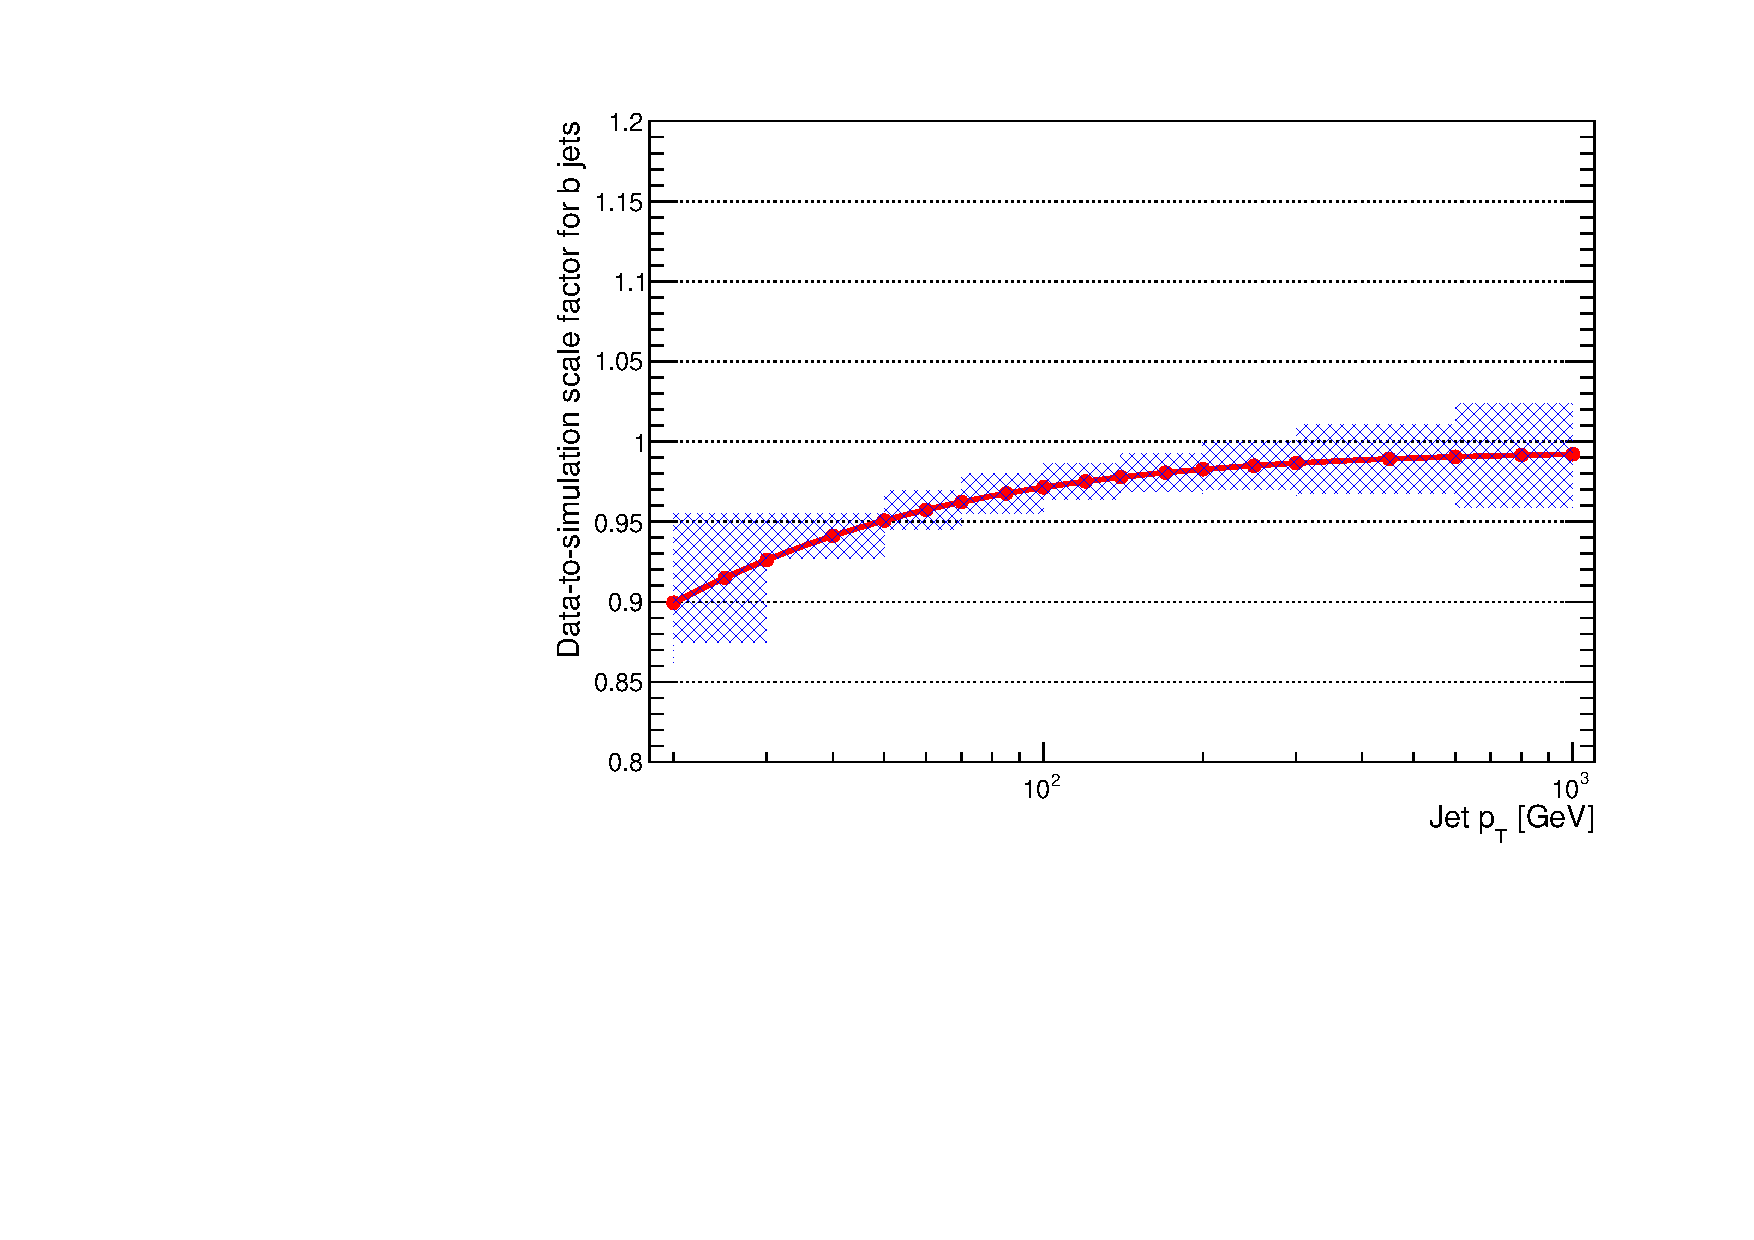
\includegraphics[angle=0,width=0.45\columnwidth]{fig/sfs_bjet.pdf}
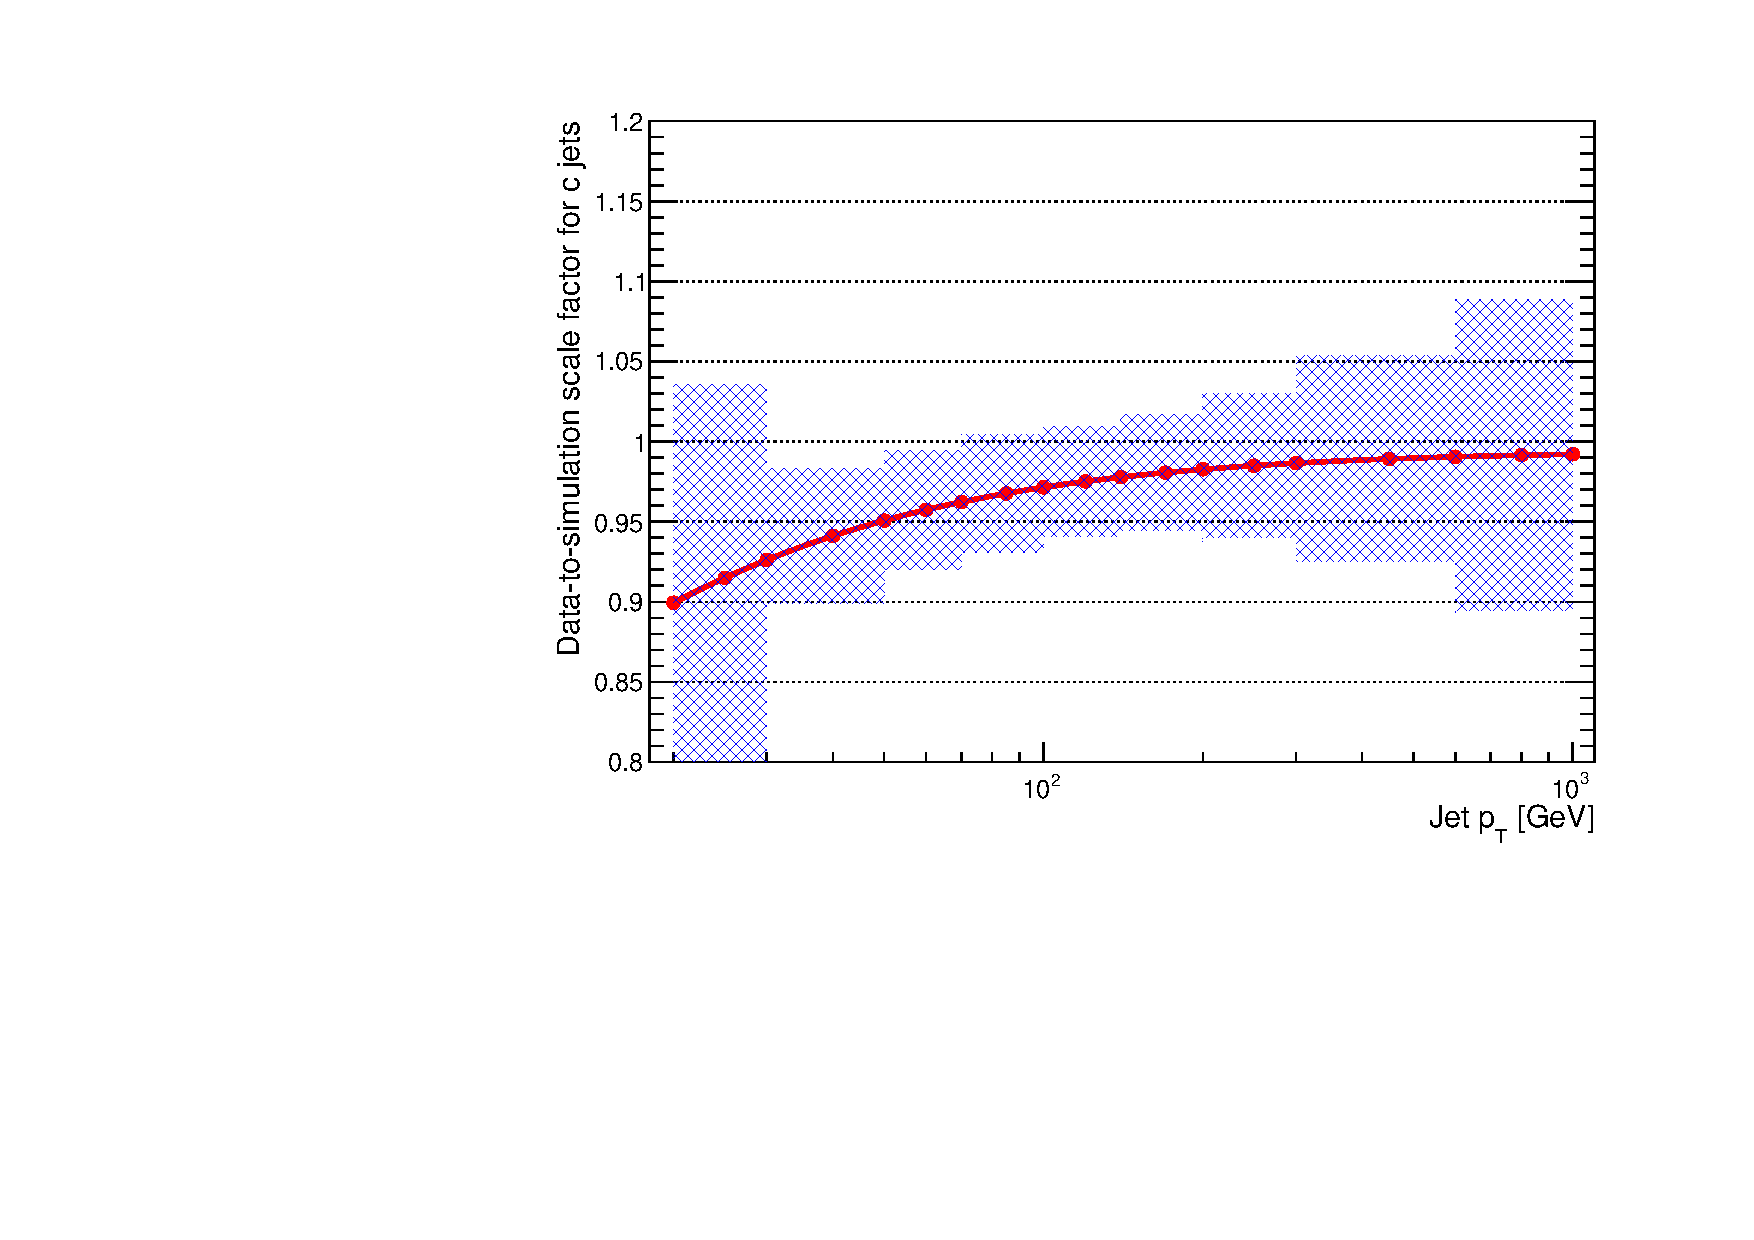
\includegraphics[angle=0,width=0.45\columnwidth]{fig/sfs_cjet.pdf}
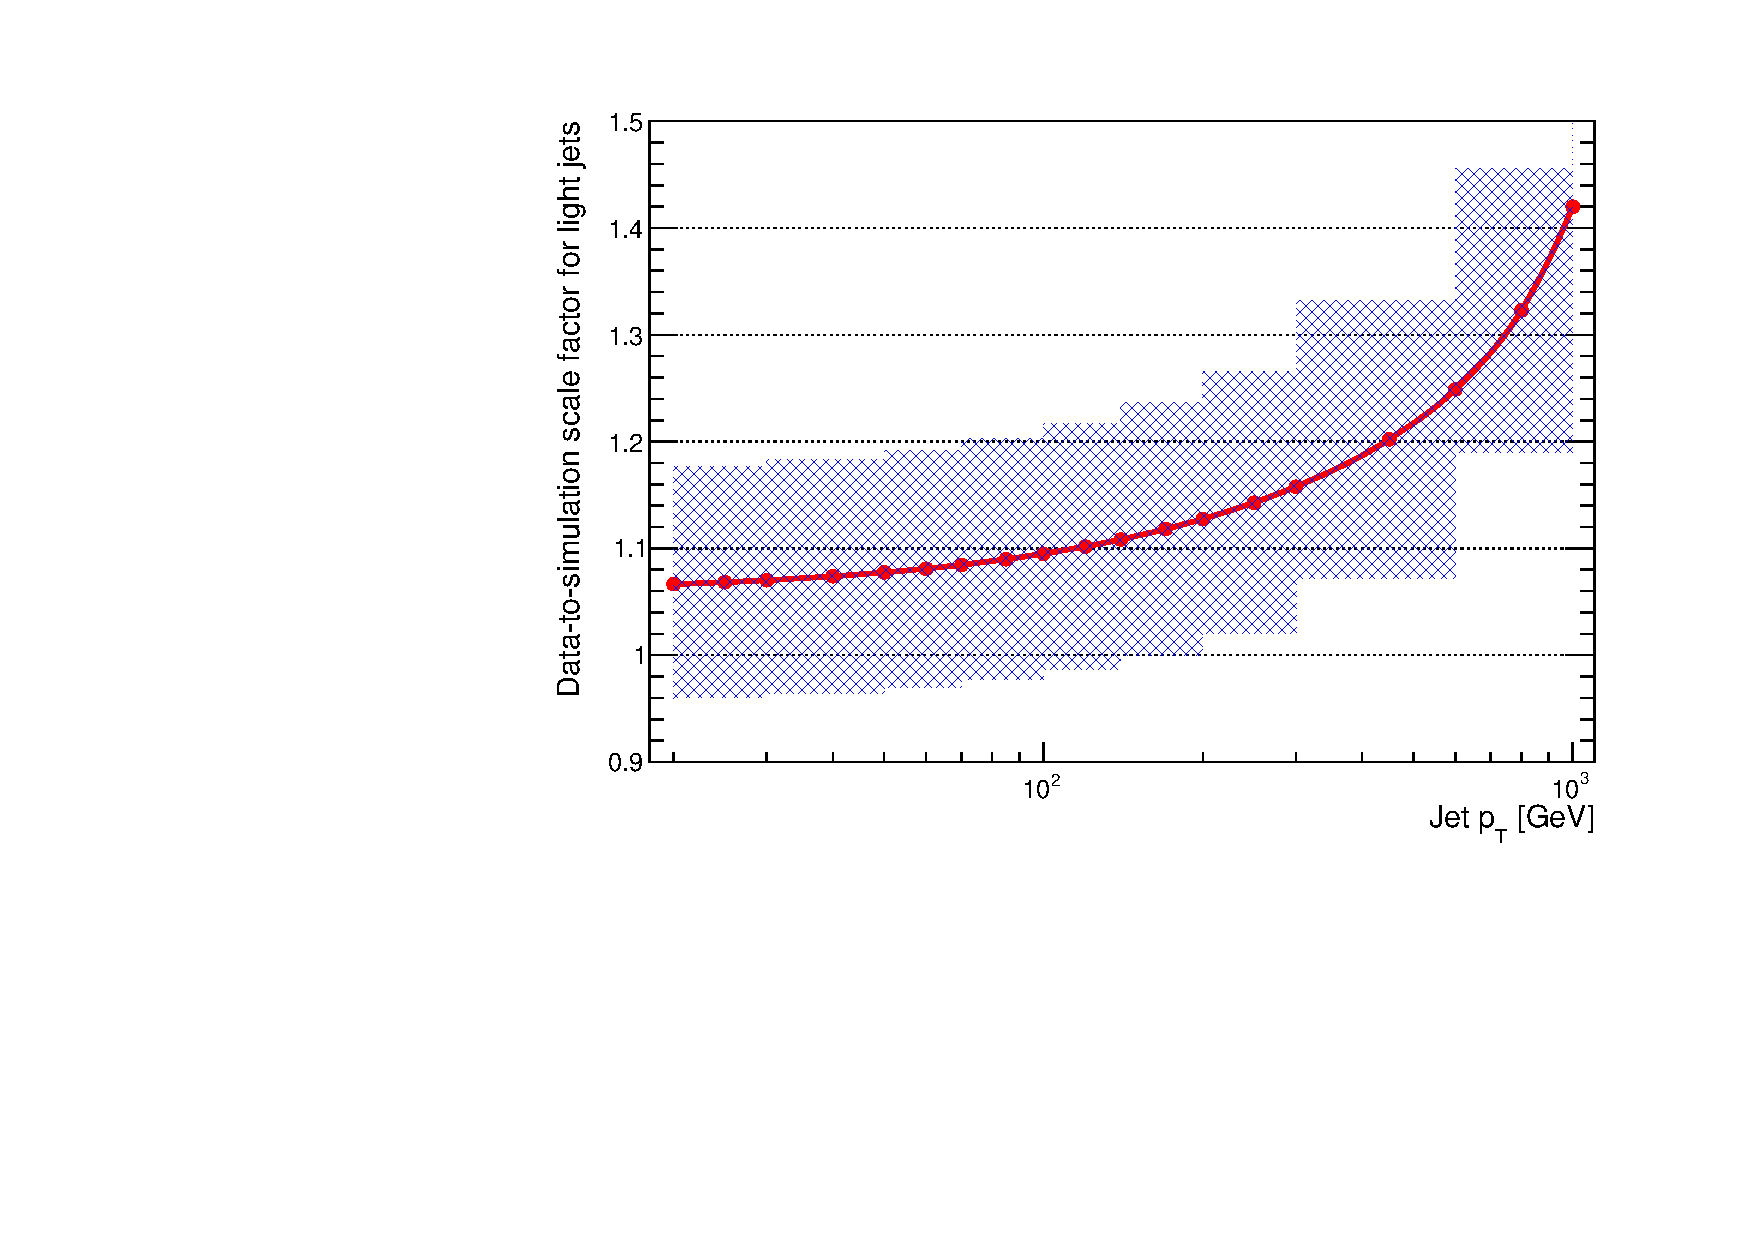
\includegraphics[angle=0,width=0.45\columnwidth]{fig/sfs_ljet.pdf}
\end{center}
\caption{The data-to-simulation scale factors for the tagging efficiency of b-flavor jets (top-left), charm-flavor jets (top-right), and light-flavor or gluon jets (bottom) are shown as a function of jet \pT.
The associated uncertainty with each scale factor is shown as a blue hashed band.}
\label{fig:bkg_sys_tables}
\end{figure}

The systematic uncertainties on the \Nb shape are assessed by the $\pm 1$~s.d.\ \Nb templates resulting from varying the SFs according to their uncertainties.
Because the b and c jet SFs have correlated uncertainties, they are conservatively varied together, creating one set of templates.
The light-flavor SFs are uncorrelated with the b and c jet SFs and are varied independently.
The effect of these variations on the \Nb distribution in \ttbar events is shown in Figure~\ref{fig:sf_bc_variations} and Figure~\ref{fig:sf_udsg_variations}.

\begin{figure}[tbp!]
\begin{center}
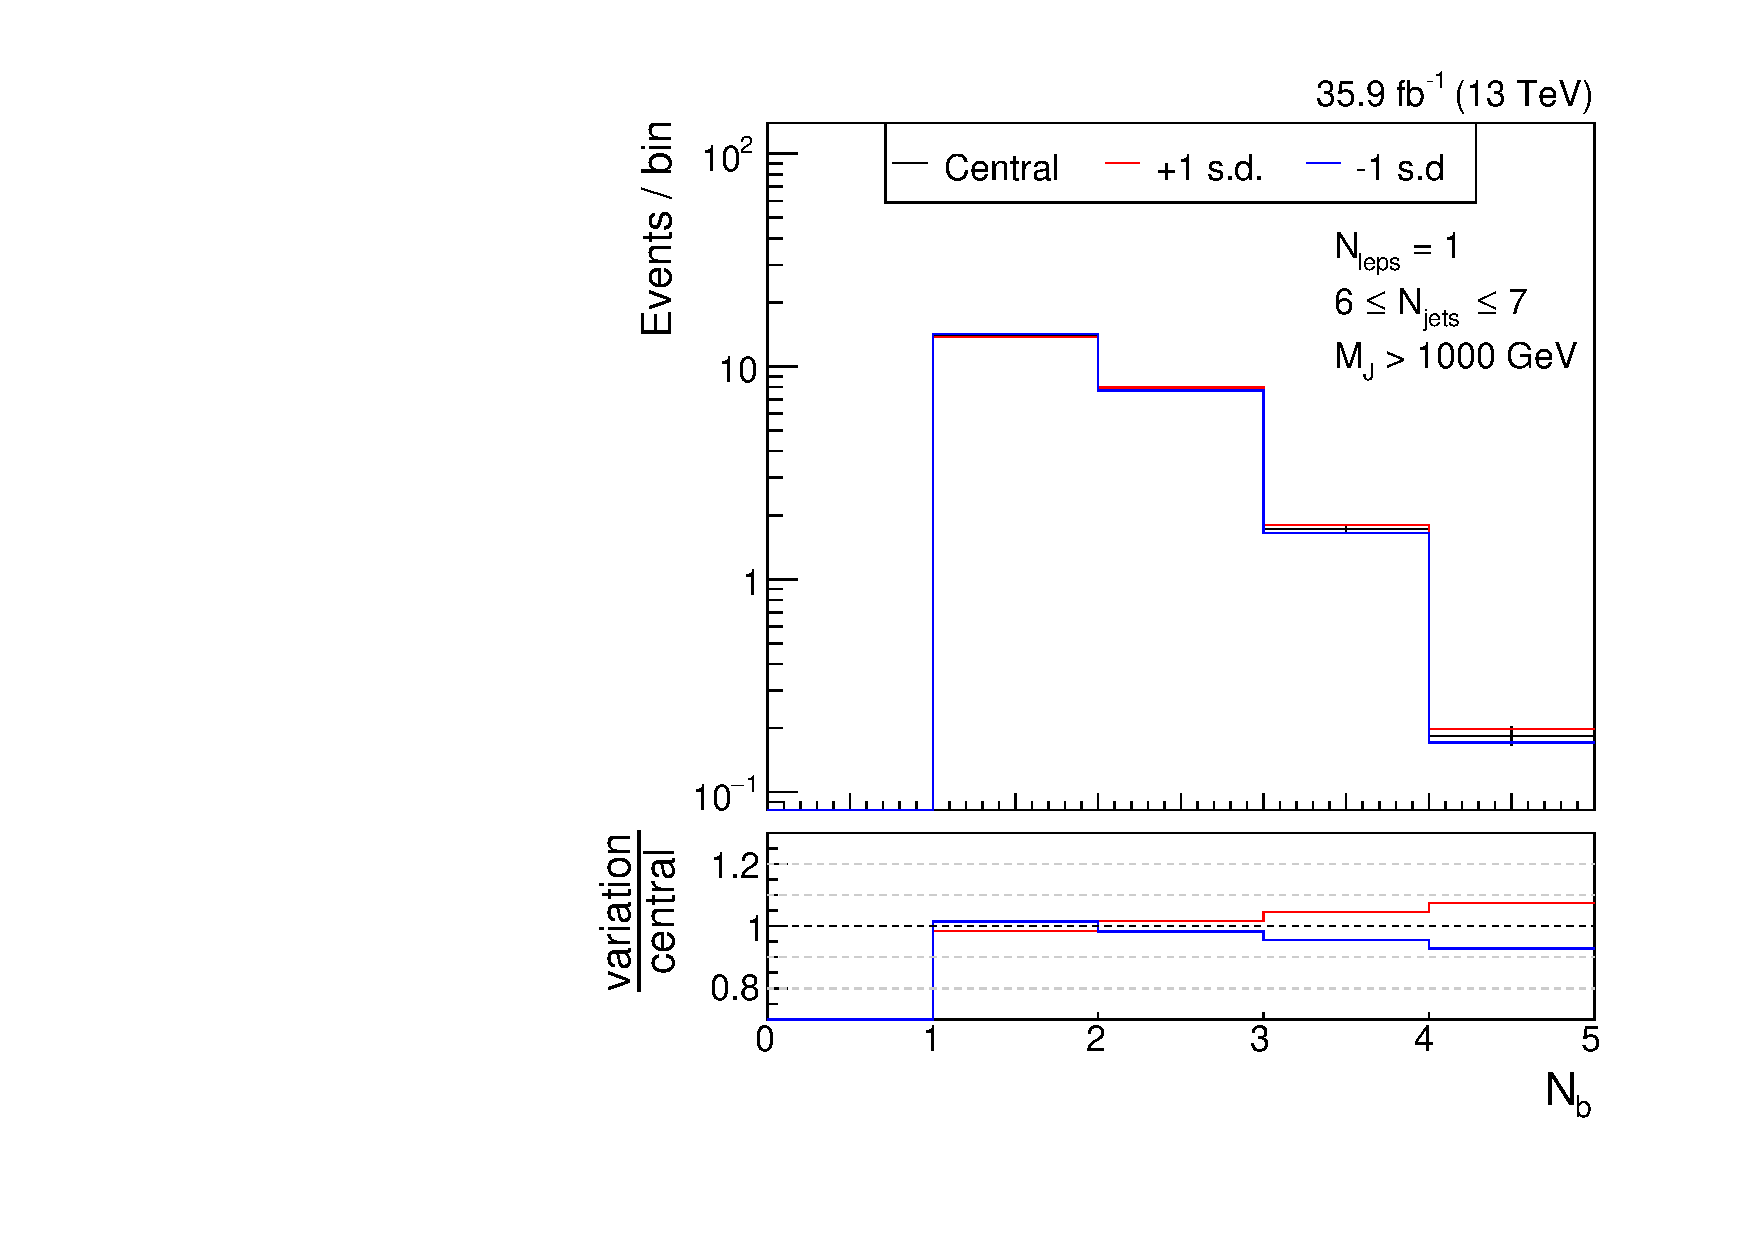
\includegraphics[angle=0,width=0.45\columnwidth]{fig/bin20_ttbar_btag_bc_mconly.pdf}
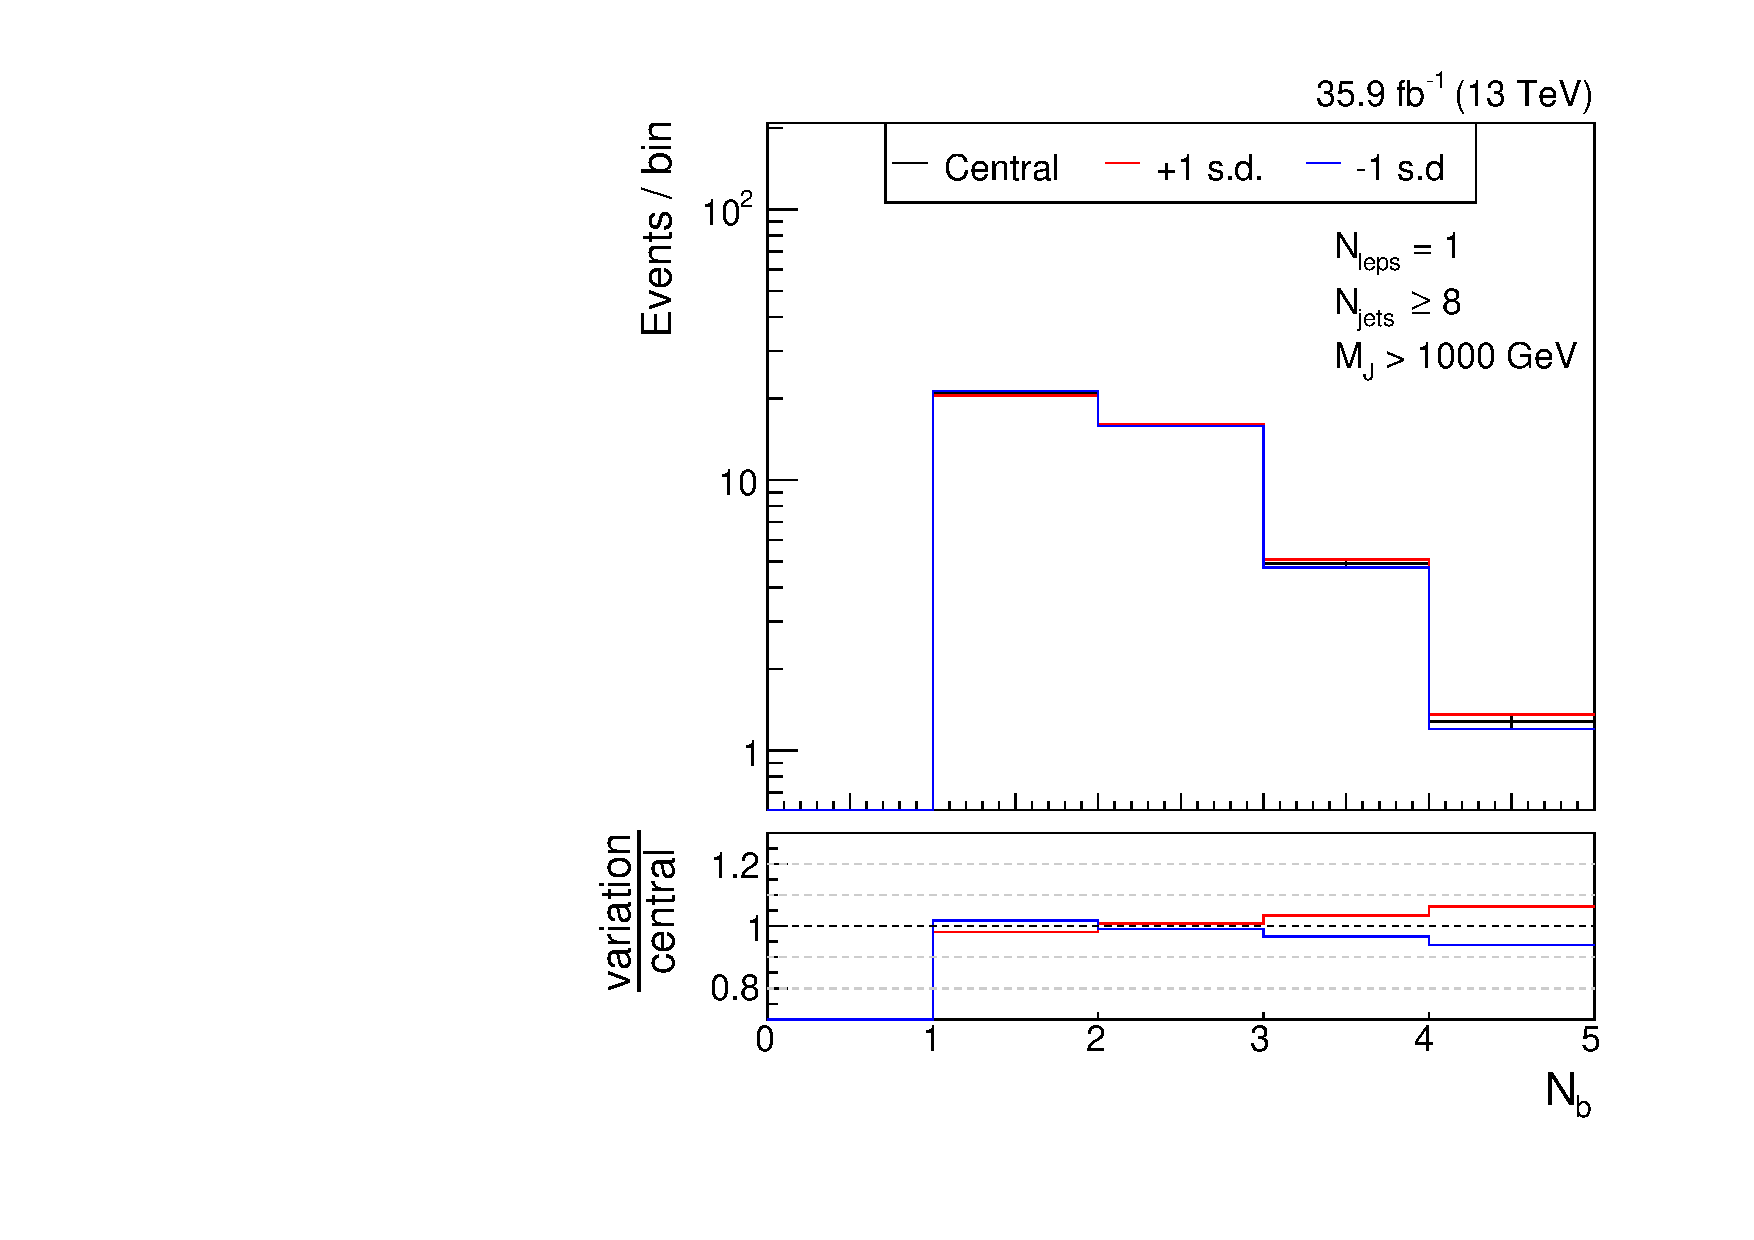
\includegraphics[angle=0,width=0.45\columnwidth]{fig/bin21_ttbar_btag_bc_mconly.pdf}
\end{center}
\caption{Effect of the $\pm 1$~s.d.\ correlated variations of the b-flavor and c-flavor jet data-to-simulation scale factors on the \Nb distribution in \ttbar for the two most sensitive bins: ($\Njets \geq 8$, $800 < \MJ \leq 1000~\GeV$) (left) and ($\Njets \geq 8$, $\MJ > 1000~\GeV$) (right).
Event yields are normalized to that expected in $35.9~\ifb$ of data.}
\label{fig:sf_bc_variations}
\end{figure}

\begin{figure}[tbp!]
\begin{center}
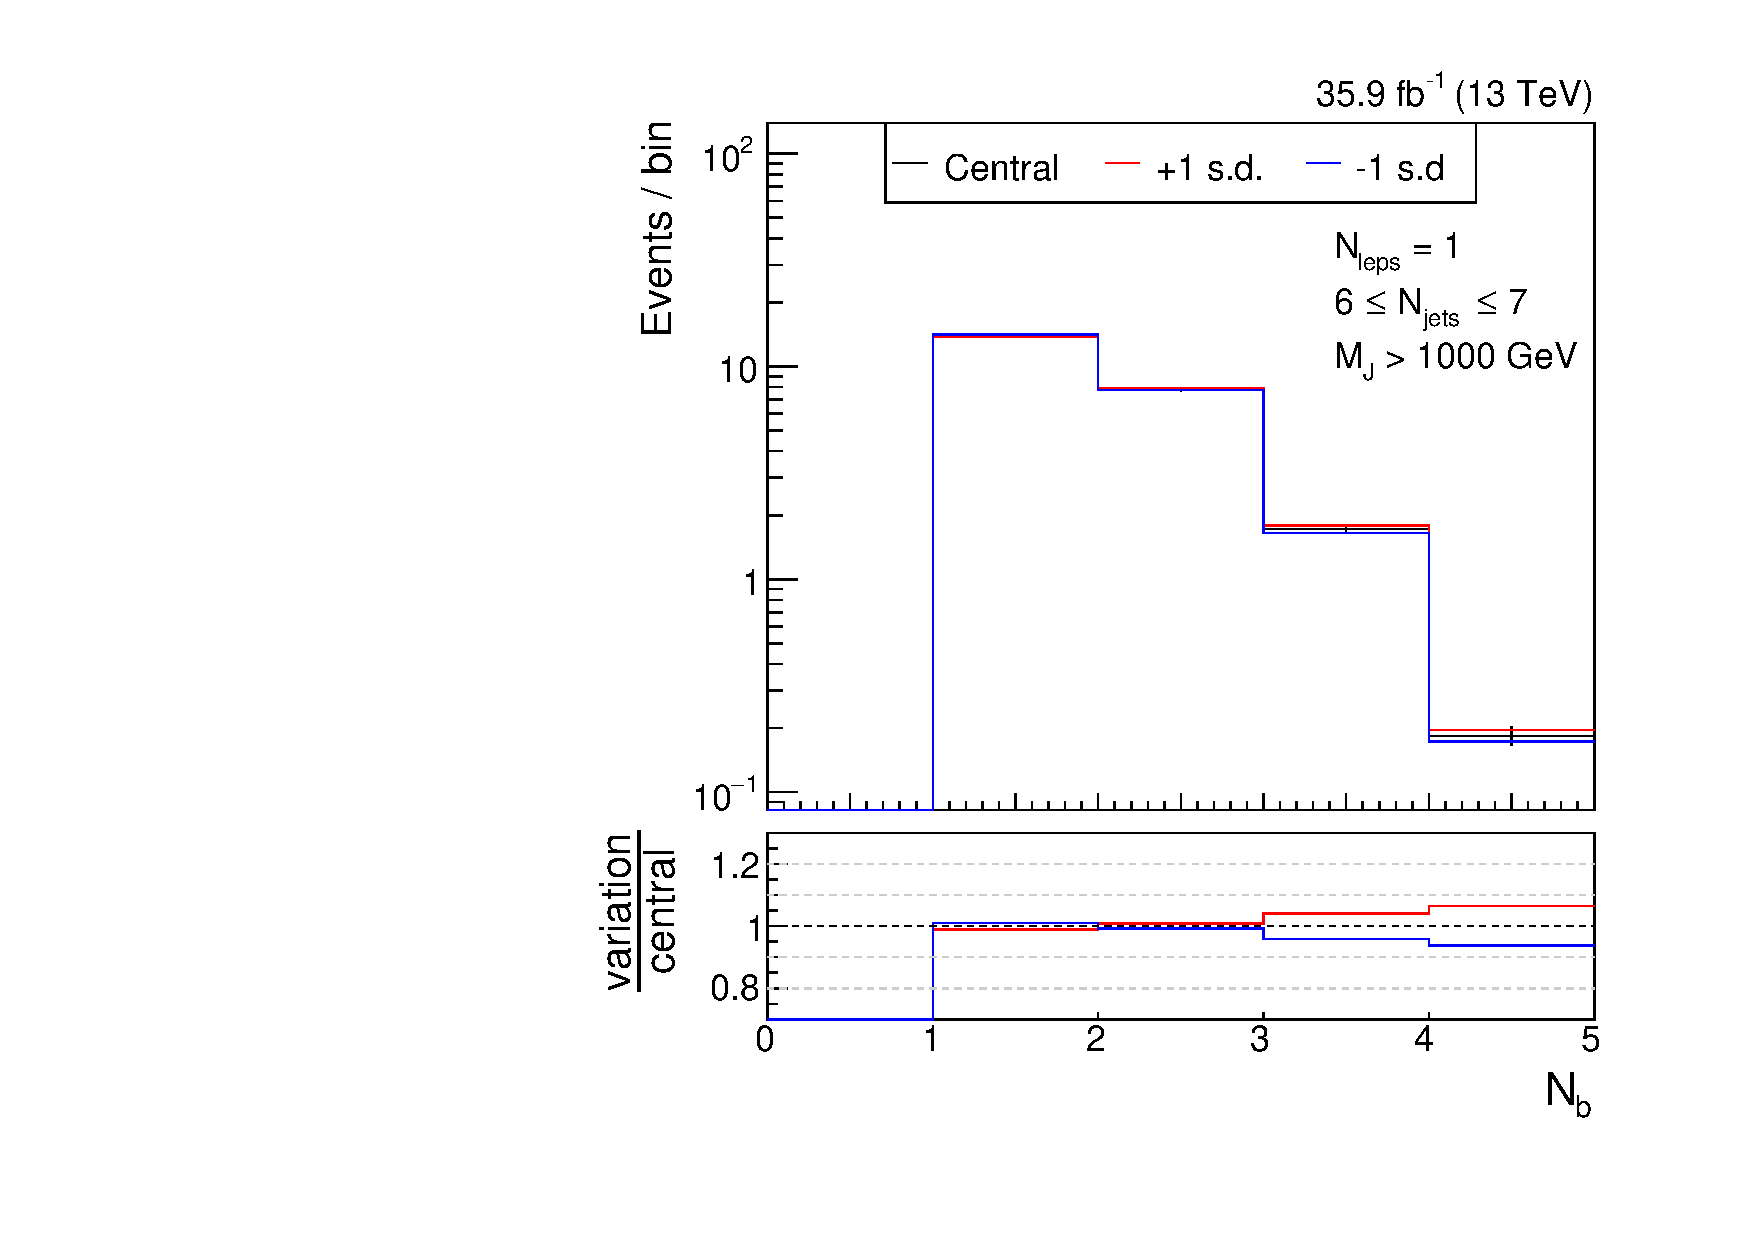
\includegraphics[angle=0,width=0.45\columnwidth]{fig/bin20_ttbar_btag_udsg_mconly.pdf}
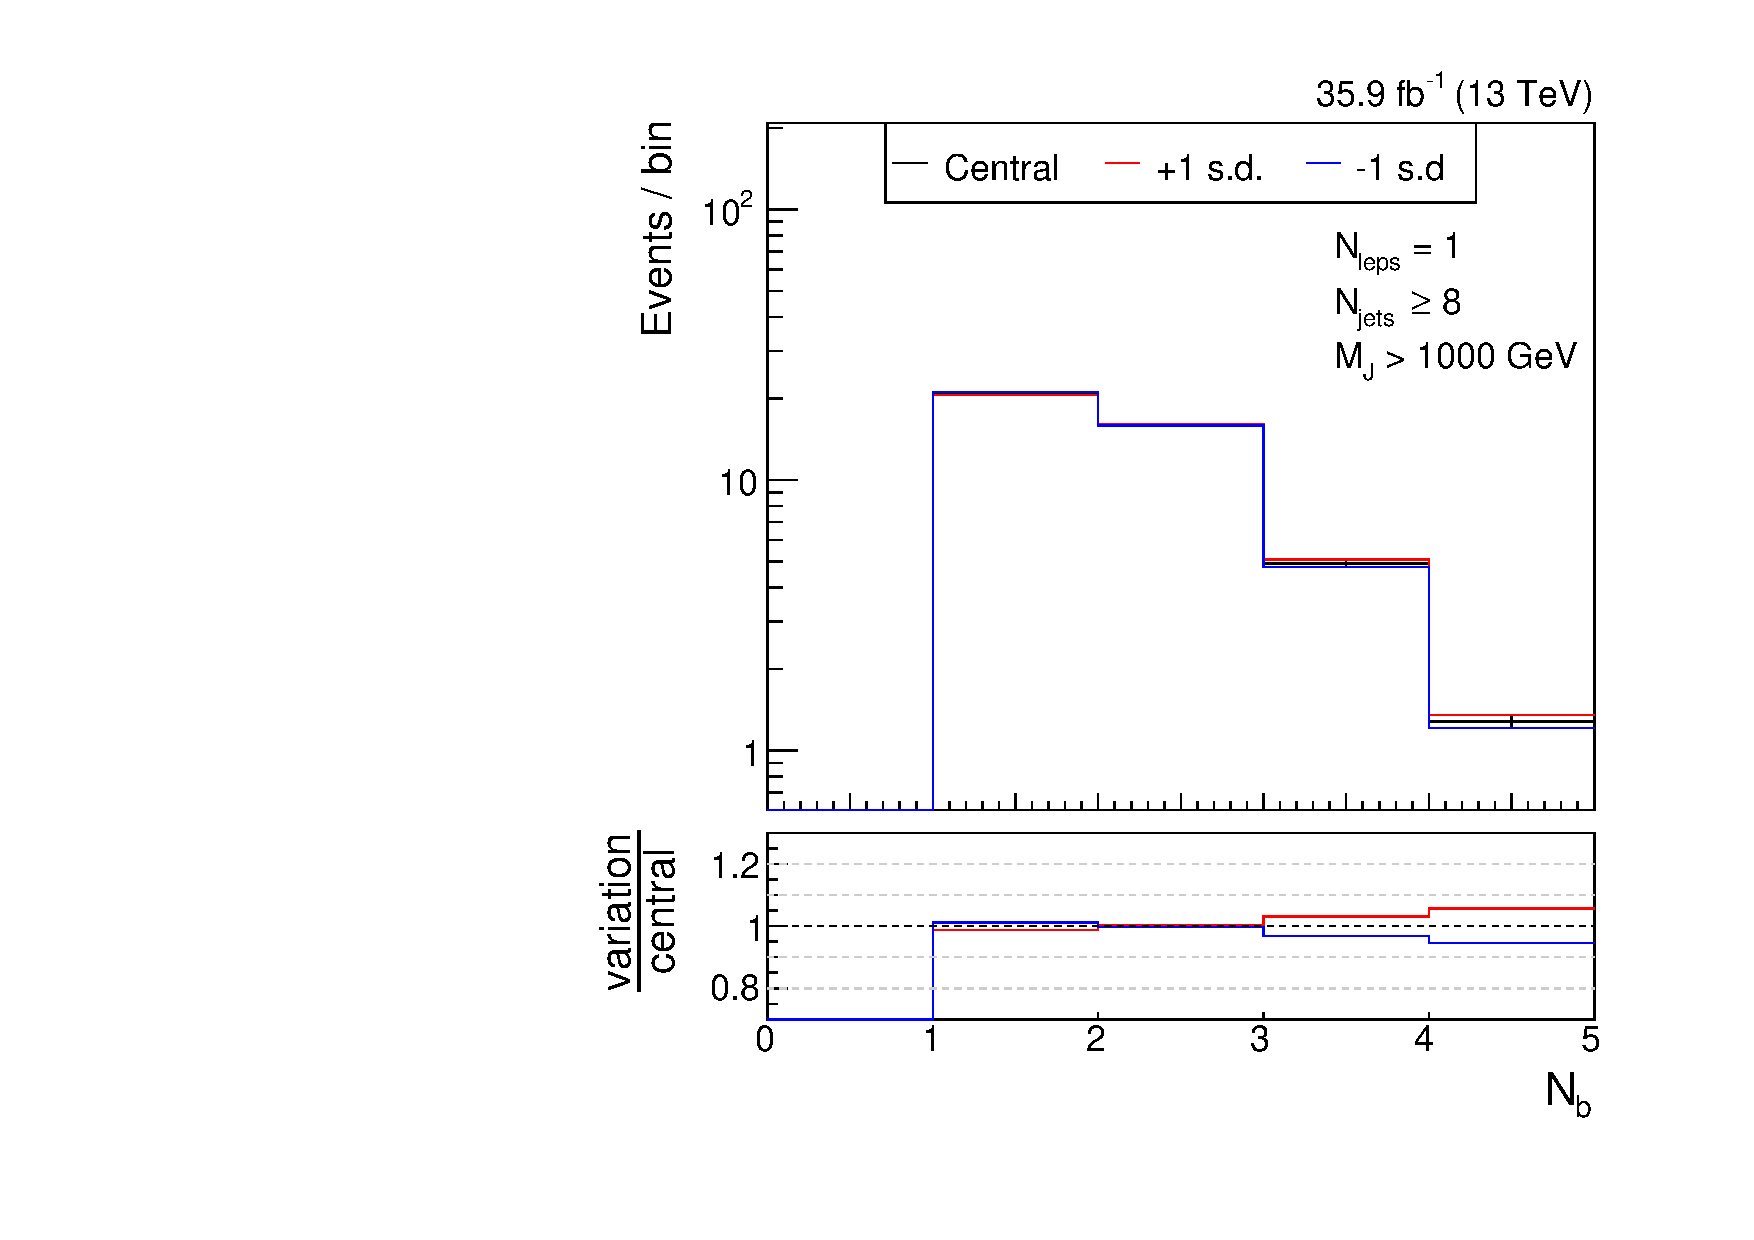
\includegraphics[angle=0,width=0.45\columnwidth]{fig/bin21_ttbar_btag_udsg_mconly.pdf}
\end{center}
\caption{Effect of the $\pm 1$~s.d.\ variations of the light-flavor jet data-to-simulation scale factors on the \Nb distribution in \ttbar for the two most sensitive bins: ($\Njets \geq 8$, $800 < \MJ \leq 1000~\GeV$) (left) and ($\Njets \geq 8$, $\MJ > 1000~\GeV$) (right).
Event yields are normalized to that expected in $35.9~\ifb$ of data.}
\label{fig:sf_udsg_variations}
\end{figure}

\end{section}

\begin{section}{Lepton Fake Rate in QCD}

While the QCD normalization is measured from data, it is mostly constrained by the $\Nleps = 0$ selection and applied in a $\Nleps = 1$ region.
If the simulated \Nleps distribution is not modelled perfectly, there may be residual differences between the normalizations of these two regions.
For processes that have true prompt leptons, such as \ttbar and \Wjets, the \Nleps distribution is well modelled, because the dominant effects are the W branching fractions and the acceptance (including selection efficiency), both of which are well understood. 
For QCD, however, this is less well modelled as the simulation of the tail of the jet fragmentation function as well as detector effects that can produce fake leptons are not as well understood.

To assign a systematic uncertainty on the modelling of the ratio of 0-lepton to 1-lepton events in QCD, the lepton isolation distributions are studied.
Figure~\ref{fig:lep_iso} shows the relative isolation distributions for eletrons (left) and muons (right) in a data sample corresponding to the control regions.
The binning of the histograms are chosen such that the first bin corresponds to the relative isolation requirement for signal leptons (0.1 for electrons and 0.2 for muons).
The normalizations of the QCD, \ttbar, and \Wjets processes are scaled to match the results of a control region fit described in Section~\ref{sec:crfit}.

\begin{figure}[tbp!]
\begin{center}
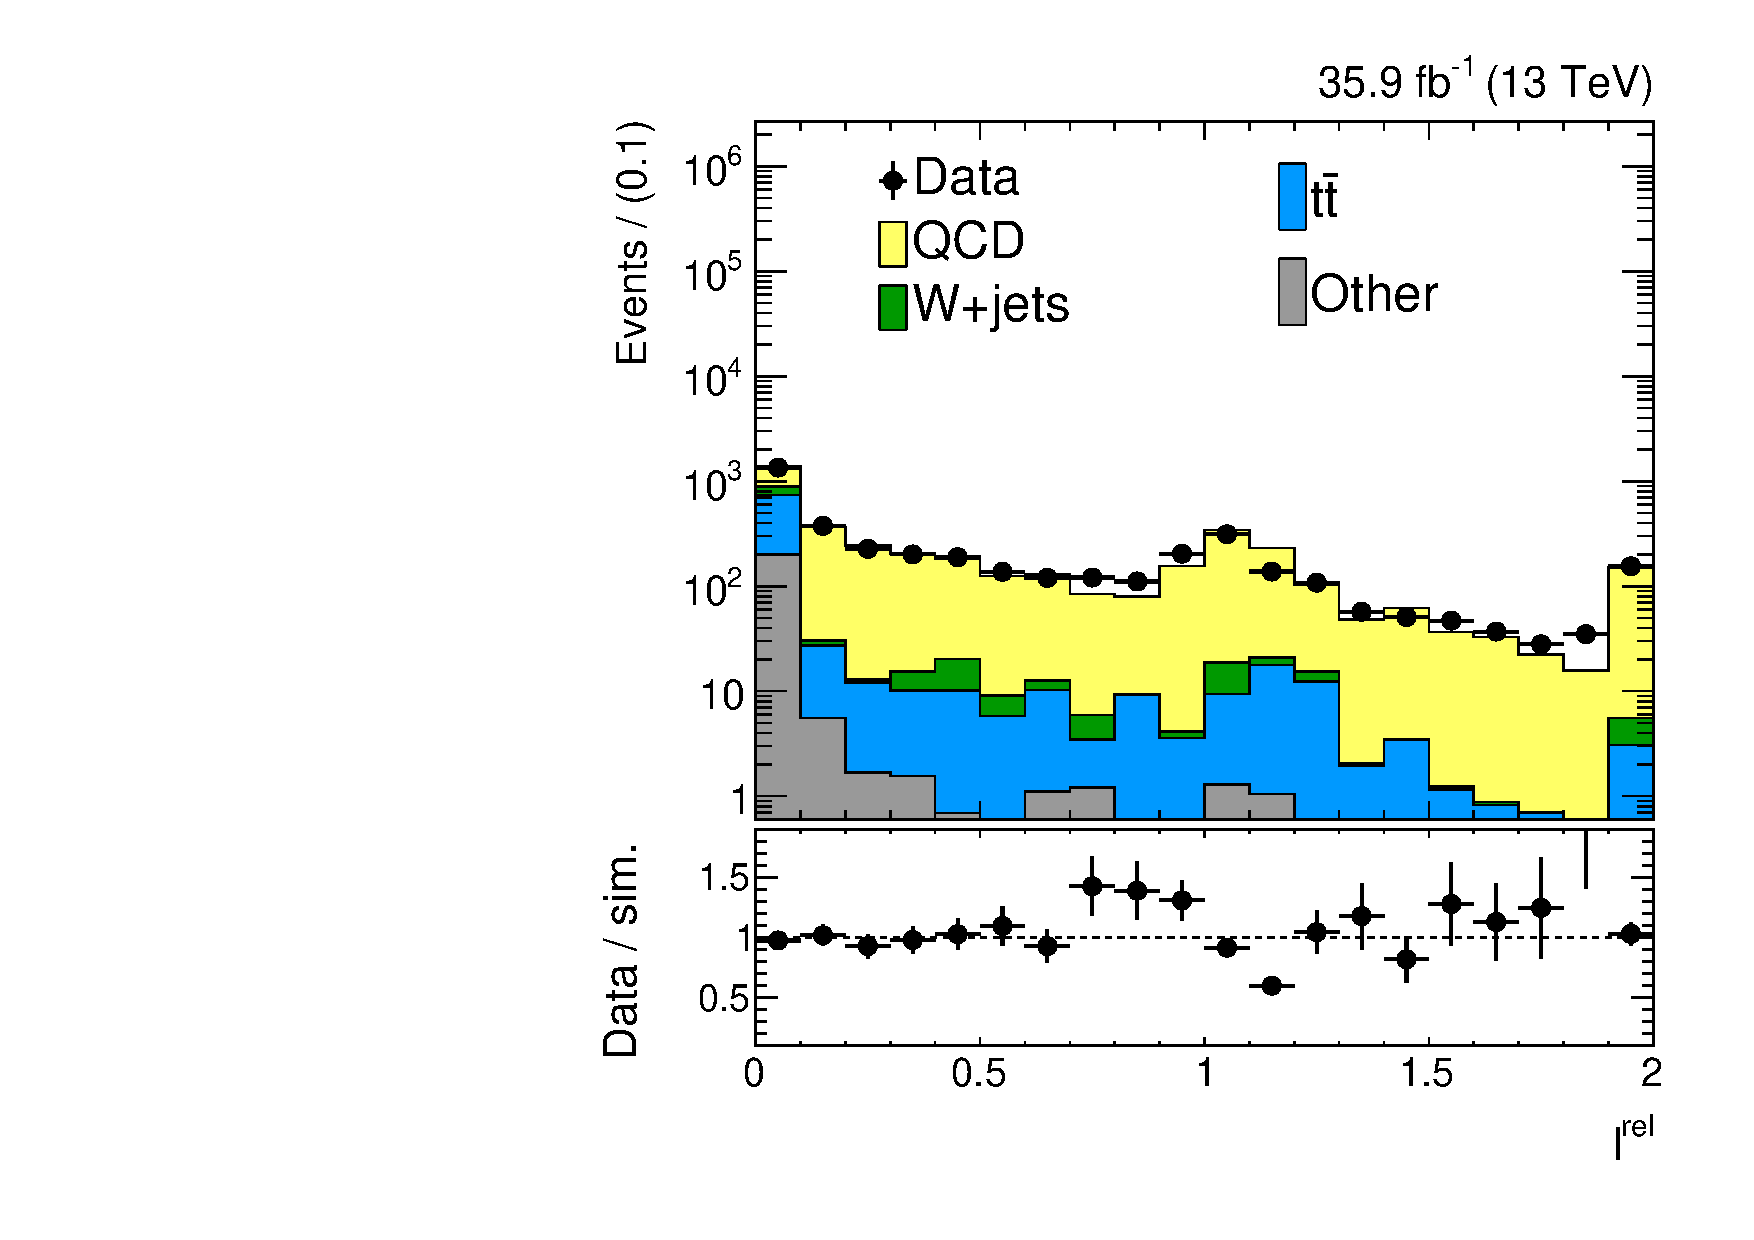
\includegraphics[angle=0,width=0.45\columnwidth]{fig/iso_els.pdf}
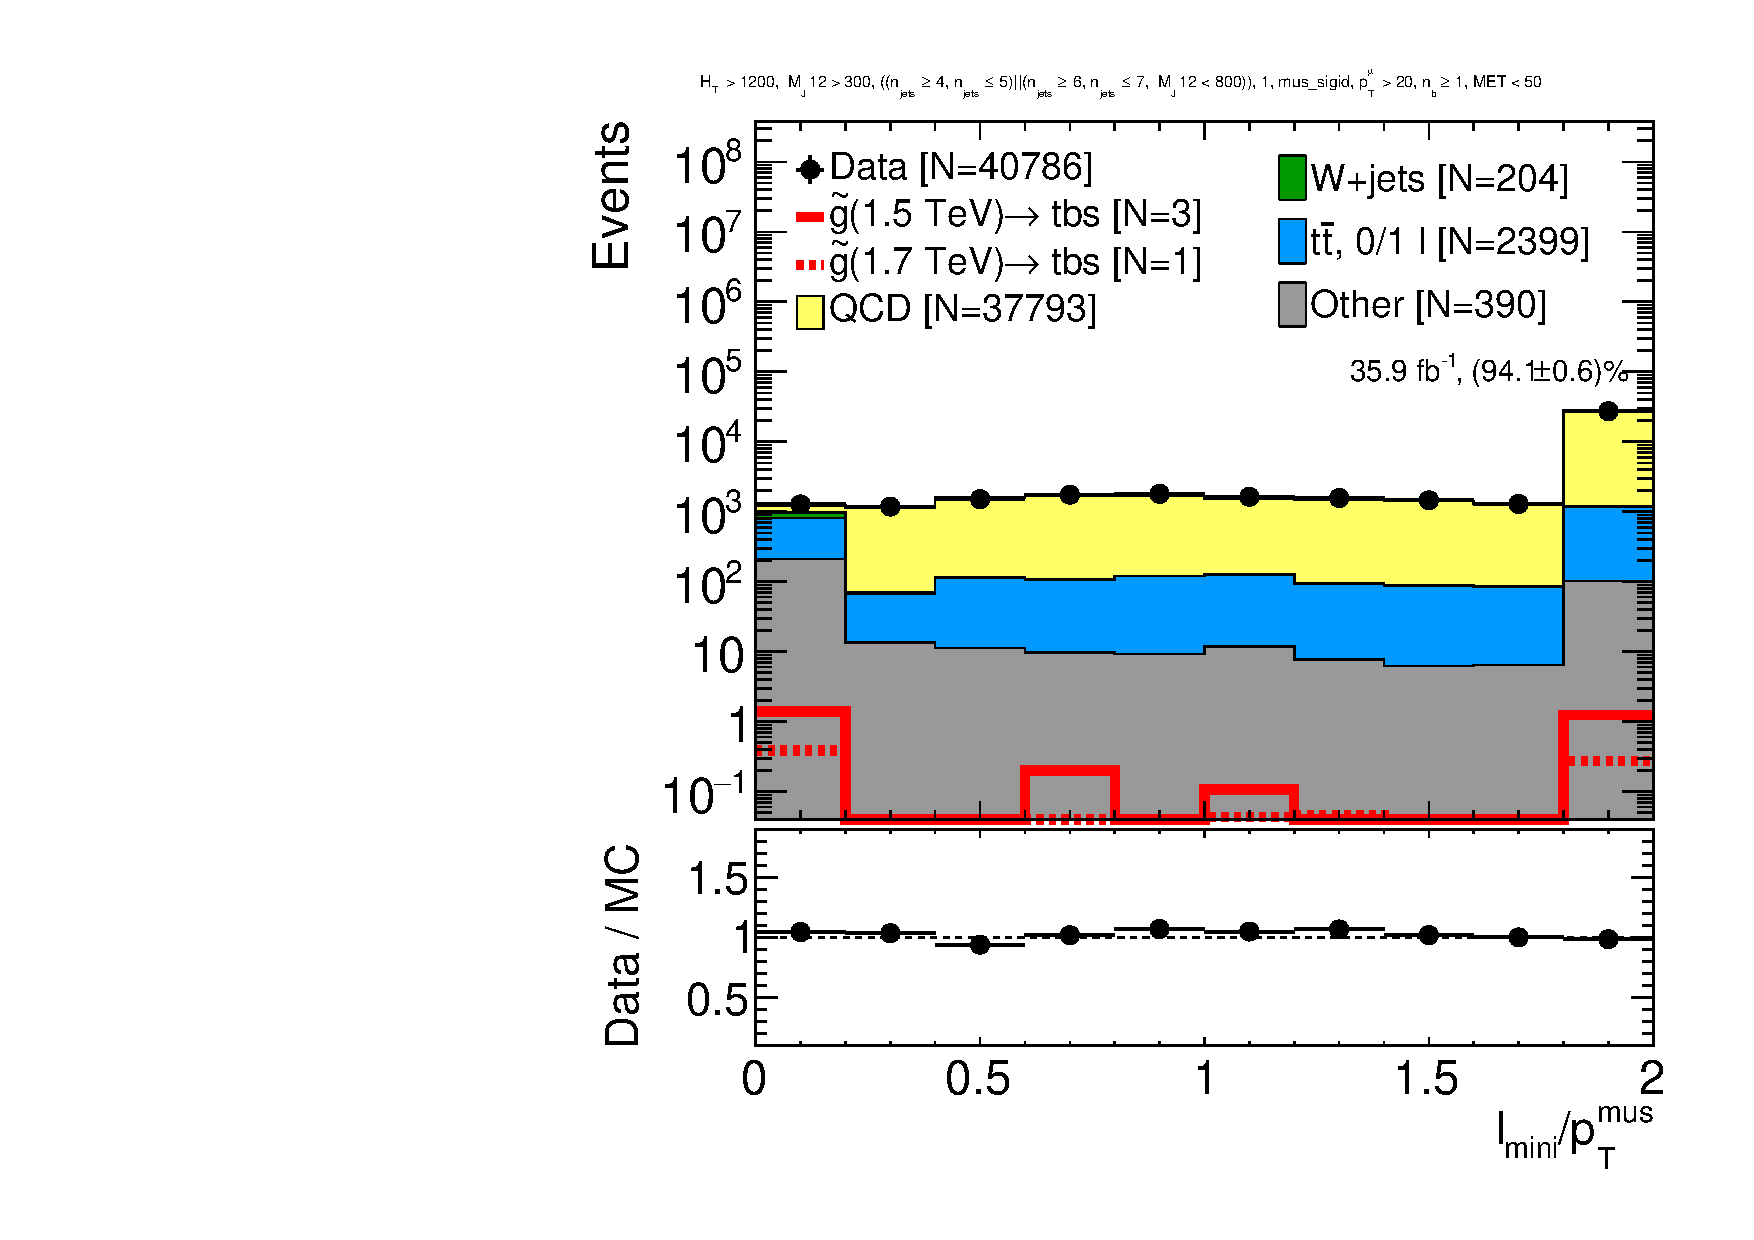
\includegraphics[angle=0,width=0.45\columnwidth]{fig/iso_mus.pdf}
\end{center}
\caption{The relative isolation distribution for electrons (left) and muons (right) in the control region bins.
The binning of the histograms are chosen such that the first bin corresponds to the relative isolation requirement for signal leptons (0.1 for electrons and 0.2 for muons).
The normalizations of the QCD, \ttbar, and \Wjets processes are scaled to match the results of a control region fit described in Section~\ref{sec:crfit}.}
\label{fig:lep_iso}
\end{figure}

Table~\ref{tab:lep_iso} shows the ratio of $I^{\mrm{rel}} < 0.1(0.2)$ to $I^{\mrm{rel}} \geq 0.1(0.2)$ for electrons(muons) in QCD and data with contributions for all other processes (\ttbar, \Wjets, Other) subtracted.
As the ratio in data agrees to that in QCD simulation within 20\%, an additional 20\% log-normal uncertainty is assigned to the QCD normalization in 1-lepton bins.

\begin{table}[h]
\centering
\begin{tabular}{l | cc|c | cc|c }
\hline\hline
\multirow{2}{*}{Process}  &  \multicolumn{3}{c|}{Electrons}                                        &  \multicolumn{3}{c}{Muons}                                        \\
                          &  $I^{\mrm{rel}} < 0.1$          &  $I^{\mrm{rel}} \geq 0.1$  & ratio  &  $I^{\mrm{rel}} < 0.2$      &  $I^{\mrm{rel}} \geq 0.2$  &  ratio \\
\hline
QCD                       &  496.8                          &  2455.5                    &  0.20  &  219.8                      &  36553.3                   & 0.0060 \\
Data - all other          &  452.8                          &  2500.5                    &  0.18  &  275.4                      &  37497.7                   & 0.0073 \\
\hline\hline
\end{tabular}
\caption{Comparison of the relative isolation distributions, as described in the caption of Figure~\ref{fig:lep_iso}, for electrons and muons between QCD and data with contributions from ``all other'' (\ttbar, \Wjets, and Other) subtracted.}
\label{tab:lep_iso}
\end{table}

\end{section}

\begin{section}{Additional systematic uncertainties}

Other experimental uncertainties are small and include lepton selection efficiency, jet energy scale, jet energy resolution, and integrated luminosity.
The uncertainty associated with lepton selection efficiency is determined by varying the efficiency to select a lepton within its uncertainty determined from data.
Jet energy scale uncertainties~\cite{Chatrchyan:2011ds,1748-0221-12-02-P02014} are assessed by varying the \pT of small-$R$ jets as a function of \pT and $\eta$.
The uncertainty arising from jet energy resolution~\cite{Chatrchyan:2011ds,1748-0221-12-02-P02014} is determined by applying an $|\eta|$-dependent factor to the jet \pT to match the jet energy resolution observed in data.
The integrated luminosity is varied according to its uncertainty of 2.5\%~\cite{CMS-PAS-LUM-17-001}, affecting only the backgrounds estimated from simulation.
No uncertainty is applied for the amount of pileup as studies have shown its effect to be negligible in this high-\HT selection.
The uncertainties due to the limited size of simulation samples are incorporated as uncorrelated nuisance parameters in the fit.

Theoretical systematic uncertainties are applied and include independent and correlated variations of the renormalization  and factorization scales.
Additionally, uncertainties on the PDF are incorporated by considering variations in the NNPDF 3.0 scheme~\cite{Ball:2014uwa}.
The size of these uncertainties is typically small as the effect of these variations is largely to modify the cross section of processes, which for the main backgrounds are constrained by data.

The background systematic uncertainties that affect the \Nb shape are shown in Figure~\ref{fig:bkg_sys_tables} for the two most sensitive search bin.

\begin{figure}[tbp!]
\begin{center}
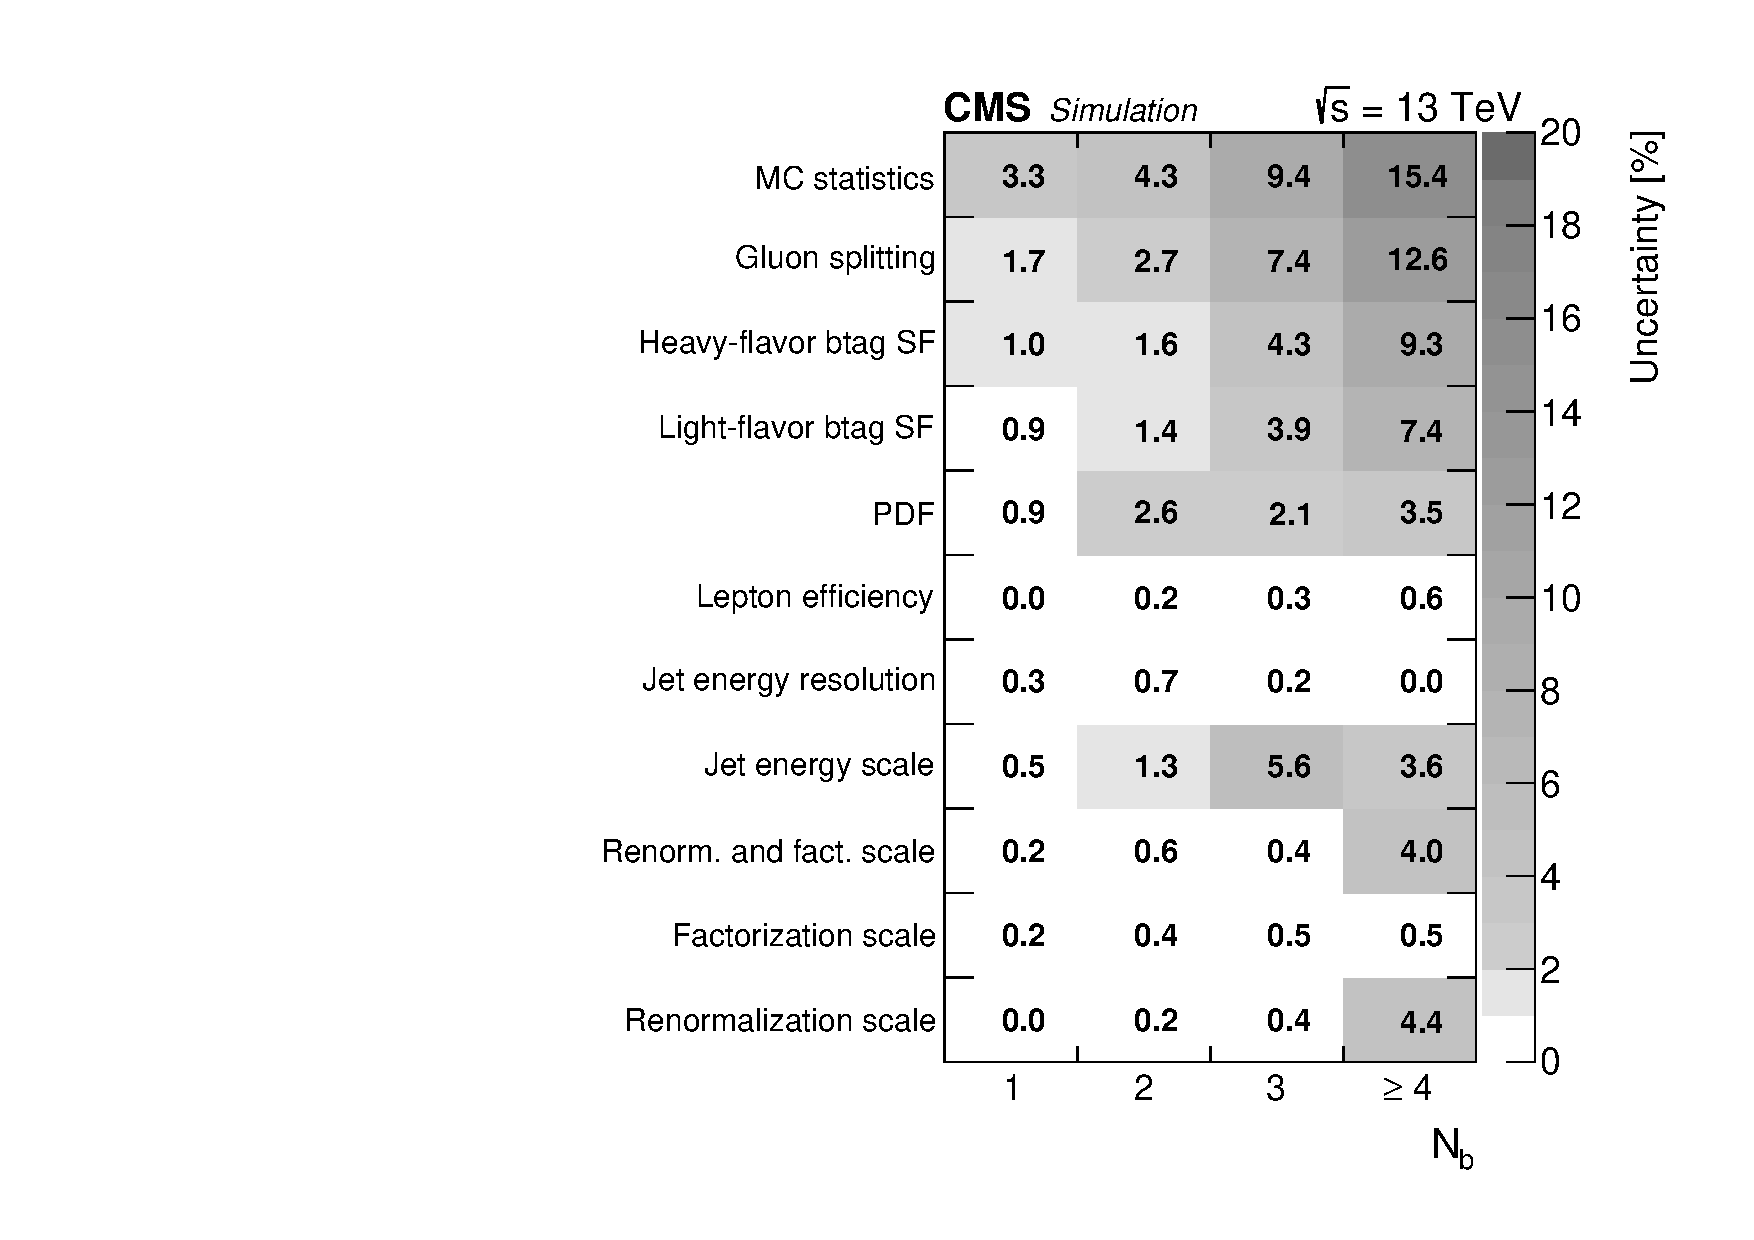
\includegraphics[angle=0,width=0.45\columnwidth]{fig/table_bkg_systs_bin20.pdf}
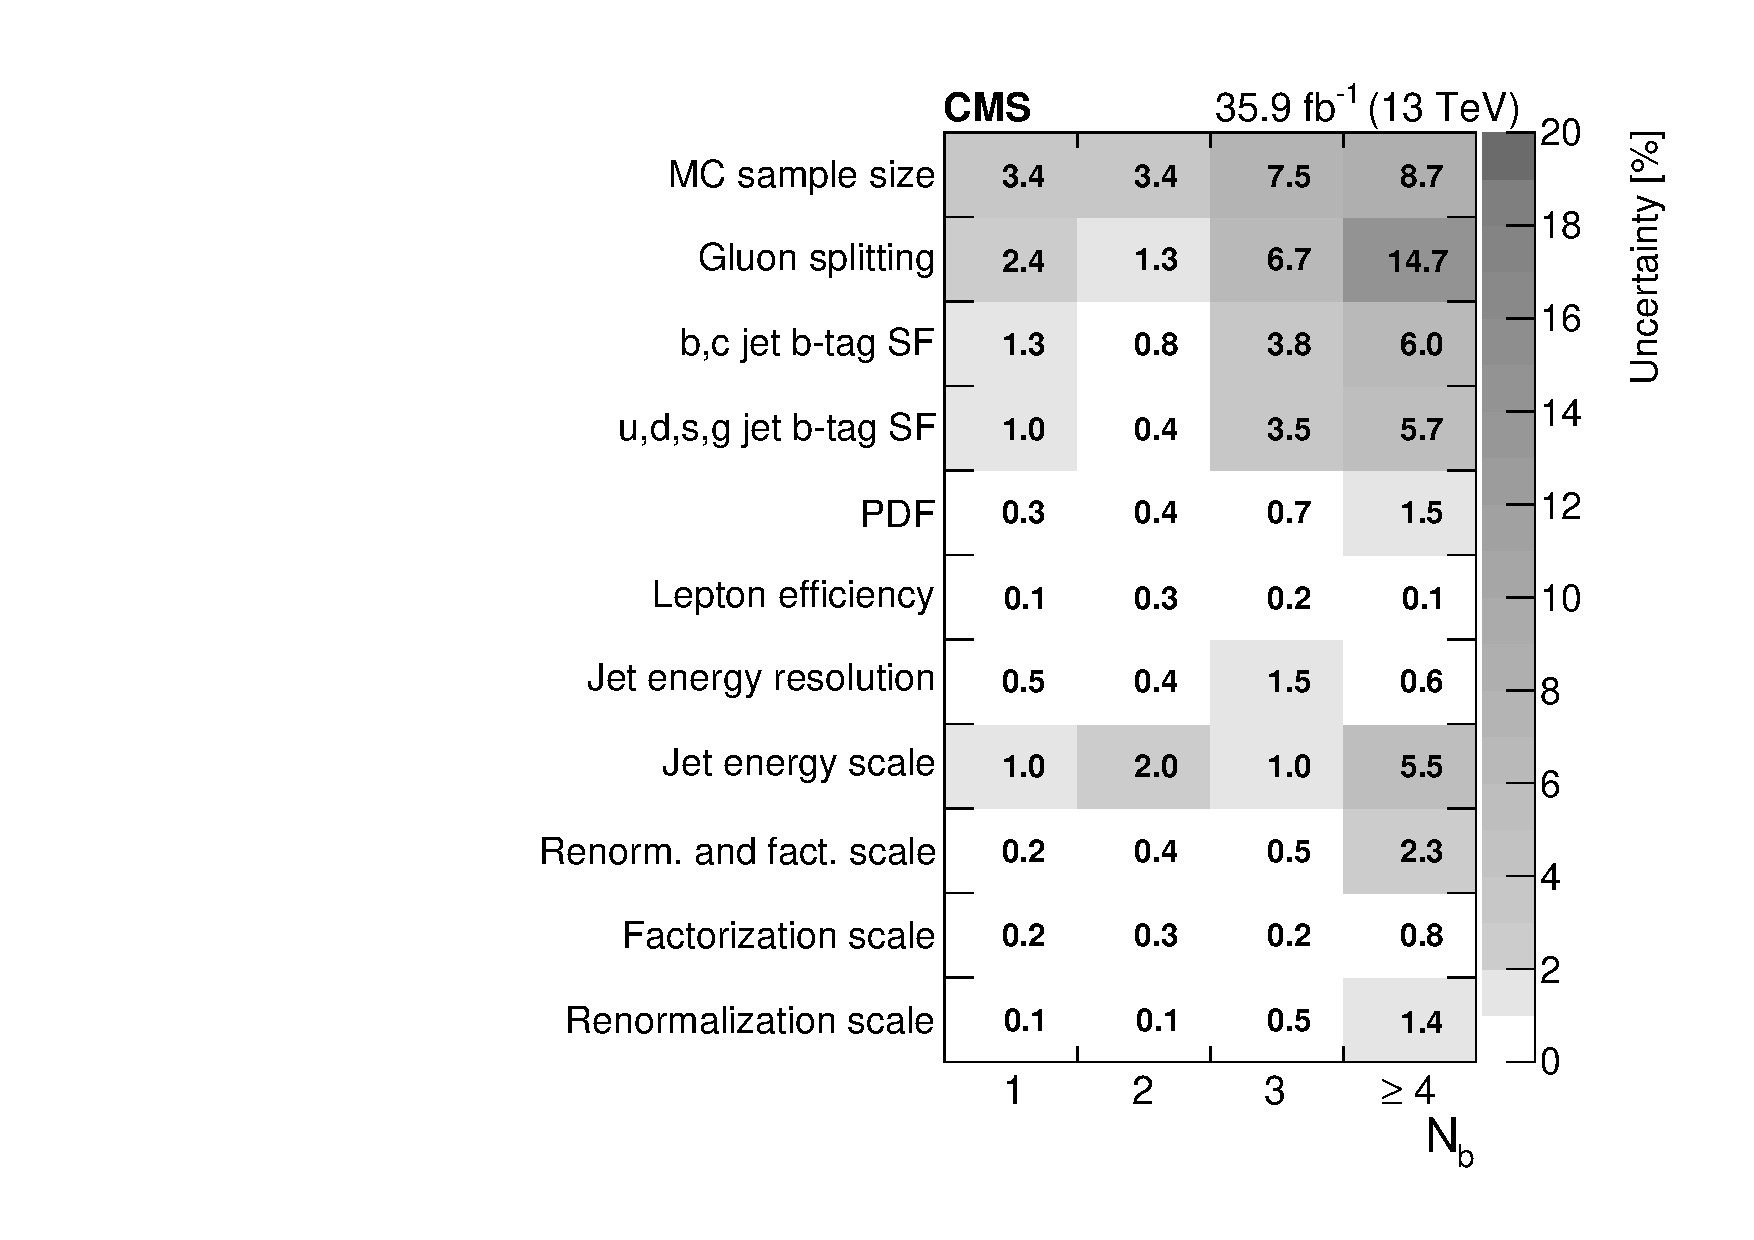
\includegraphics[angle=0,width=0.45\columnwidth]{fig/table_bkg_systs_bin21.pdf}
\end{center}
\caption{Background systematic uncertainties affecting the \Nb shape (in percent) for the ($\Njets \geq 8$, $500 < \MJ \leq 1000~\GeV$) (left) and ($\Njets \geq 8$, $\MJ > 1000~\GeV$) (right) bins.
The bottom row shows the total uncertainty for a given \Nb bin by summing in quadrature all uncertainties.
These values are similar for other (\Njets, \MJ) bins.}
\label{fig:bkg_sys_tables}
\end{figure}

\end{section}

\begin{section}{Signal Systematics}

Several of the systematic uncertainties affecting the signal yield are evaluated in the same way as the background yield.
These are the uncertainties due to gluon splitting, lepton selection efficiency, jet energy scale, jet energy resolution, b~tagging scale factors, simulation sample size, integrated luminosity, and theoretical uncertainties.
All systematic variations affect both the \Nb shape and normalization, except for the gluon splitting uncertainty, which is taken to affect only the \Nb shape.

The number of jets from ISR produced in the signal simulation is reweighted based on comparisons between data and simulated \ttbar samples.
The reweighting factors vary between 0.92 and 0.51 for the number of ISR jets between 1 and $\ge6$.
One half of the deviation from unity is taken as the systematic uncertainty in these reweighting factors.

The systematic uncertainties affecting the signal \Nb shape are shown in Fig.~\ref{fig:sig_sys_tables} (right) for the most sensitive bin in a model with $m_{\glu} = 1600~\GeV$.
The dominant signal systematic uncertainties arise from the limited simulation sample size, the b~tagging efficiency scale factors, and the ISR modeling.
There is no systematic uncertainty taken for pileup reweighting, as the signal efficiency is found to be insensitive to the number of pileup interactions, which is shown in Table~\ref{tab:sig_pu_dependence}.

\begin{figure}[tbp!]
\begin{center}
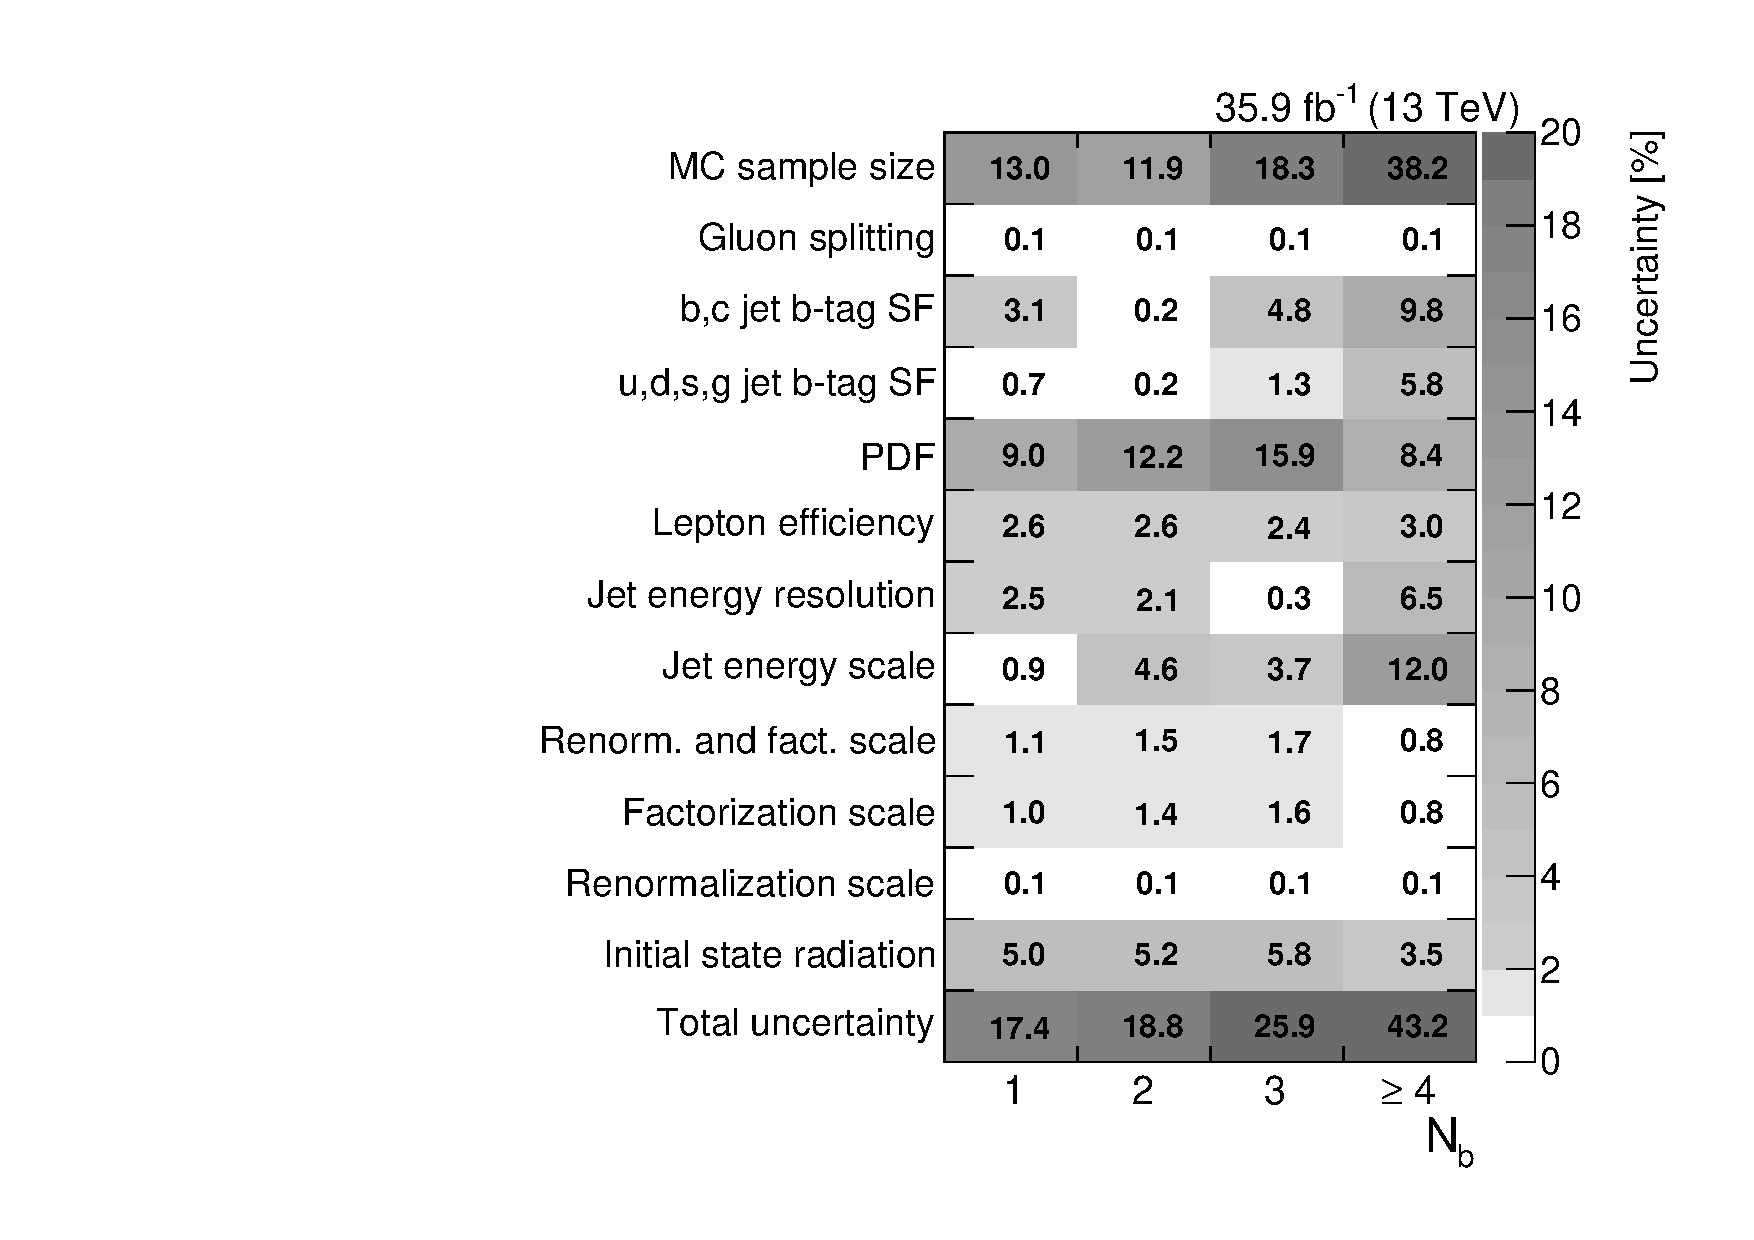
\includegraphics[angle=0,width=0.45\columnwidth]{fig/table_sig_systs_bin20_m1600.pdf}
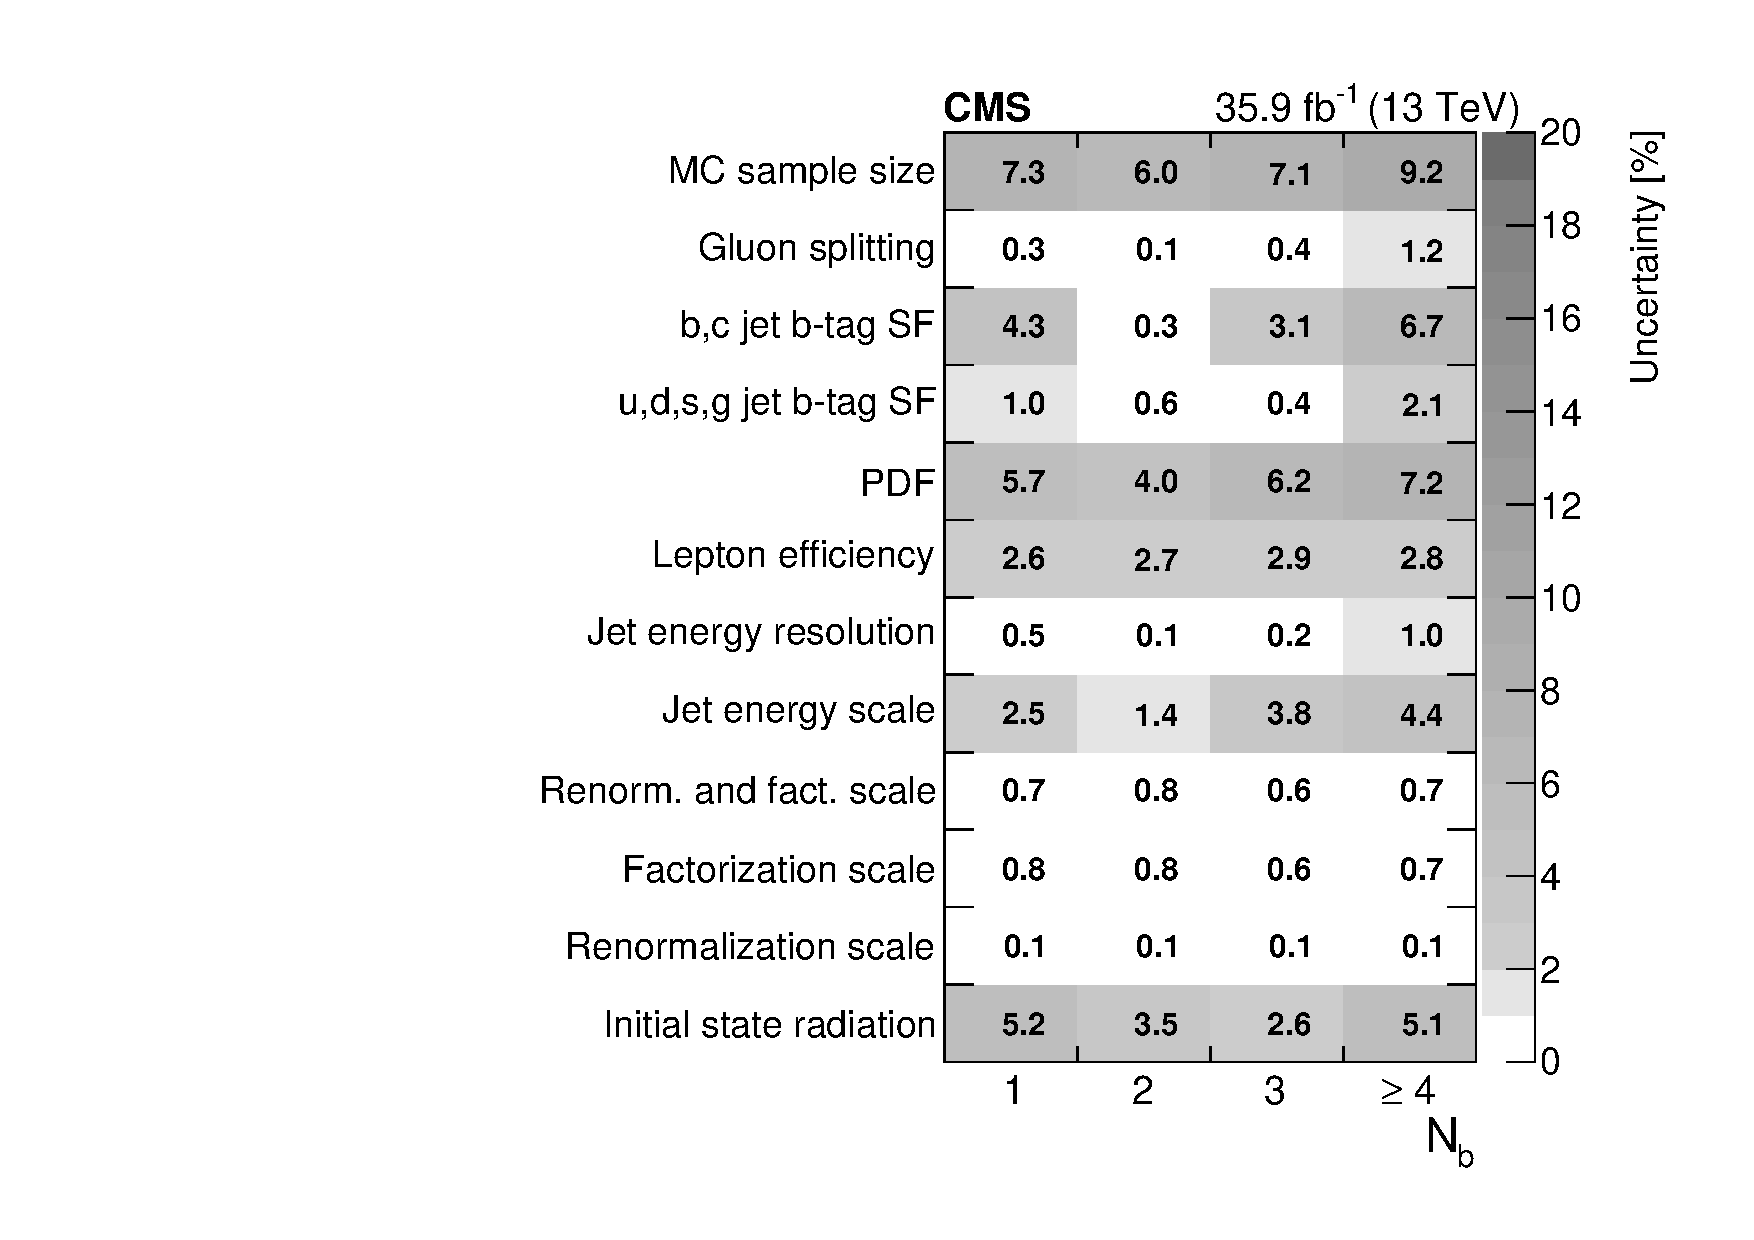
\includegraphics[angle=0,width=0.45\columnwidth]{fig/table_sig_systs_bin21_m1600.pdf}
\end{center}
\caption{Signal systematic uncertainties affecting the \Nb shape (in percent) for the ($\Njets \geq 8$, $500 < \MJ \leq 1000~\GeV$) (left) and ($\Njets \geq 8$, $\MJ > 1000~\GeV$) (right) bins.
The bottom row shows the total uncertainty for a given \Nb bin by summing in quadrature all uncertainties.
These values are similar for other (\Njets, \MJ) bins.}
\label{fig:sig_sys_tables}
\end{figure}

\begin{table}[tbp!]
\centering
\begin{tabular}{ |c|c|c| }
\hline
$N_{PV}^{true} \leq 20$ & $20 < N_{PV}^{true} \leq 40$ & $N_{PV}^{true} > 40$ \\ \hline
$8.0 \pm 0.5\%$ & $8.1 \pm 0.4\%$ & $7.5 \pm 1.5\%$ \\ \hline
\end{tabular}
\caption{The signal efficiency of the most sensitive bin ($\Njets \geq 8$, $\MJ > 1000~\GeV$) for a 1600~\GeV gluino in various bins of the number of truth-level primary vertices.}
\label{tab:sig_pu_dependence}
\end{table}

\end{section}

%TO DO
% 1. Check plot aesthetics since taken from AN, e.g. Preliminary -> Simulation
% 2. Gluon splitting shape plot with better range. (Check analysis/CWR comments or early version of paper).
% 3. Are categories GS -> qq -> 2 b-tagged jets or GS -> bb -> 2 b-tagged jets, etc
% 4. Add finer binned gs fit results plot.
% 5. Add plots for b-tag SF variation in ttbar
% 6. Expand ``other systematics'' section by going into detail about the lepton fake rate.
% 7. Use updated table for bkg sys that has the total uncertainty row.
% 8. Expand insensitivity on the pileup dependence with CWR explanation of why it doesn't matter.
% 9. Expand SF systematic section by discussing the Run split SFs.
% 10. Define \dR if not defined earlier in the document.

\chapter{Fit Validation}
\begin{section}{Section Title}

Lorem ipsum dolor sit amet, consectetur adipiscing elit, sed do eiusmod tempor incididunt ut labore et dolore magna aliqua. Ut enim ad minim veniam, quis nostrud exercitation ullamco laboris nisi ut aliquip ex ea commodo consequat. Duis aute irure dolor in reprehenderit in voluptate velit esse cillum dolore eu fugiat nulla pariatur. Excepteur sint occaecat cupidatat non proident, sunt in culpa qui officia deserunt mollit anim id est laborum.

\end{section}

\chapter{Results and Interpretation}
\begin{section}{Section Title}

Lorem ipsum dolor sit amet, consectetur adipiscing elit, sed do eiusmod tempor incididunt ut labore et dolore magna aliqua. Ut enim ad minim veniam, quis nostrud exercitation ullamco laboris nisi ut aliquip ex ea commodo consequat. Duis aute irure dolor in reprehenderit in voluptate velit esse cillum dolore eu fugiat nulla pariatur. Excepteur sint occaecat cupidatat non proident, sunt in culpa qui officia deserunt mollit anim id est laborum.

\end{section}

\chapter{Conclusions}
\begin{section}{Section Title}

Lorem ipsum dolor sit amet, consectetur adipiscing elit, sed do eiusmod tempor incididunt ut labore et dolore magna aliqua. Ut enim ad minim veniam, quis nostrud exercitation ullamco laboris nisi ut aliquip ex ea commodo consequat. Duis aute irure dolor in reprehenderit in voluptate velit esse cillum dolore eu fugiat nulla pariatur. Excepteur sint occaecat cupidatat non proident, sunt in culpa qui officia deserunt mollit anim id est laborum.

\end{section}


%=== Appendix ============================================
\part{Appendix}
\appendix
\dsp

\chapter{Mitagating the HIP Effect }{\label{appendix:a}}
\begin{section}{Section Title}

Appendicitis

\end{section}

\chapter{QCD Flavor Fit }{\label{appendix:b}}
\begin{section}{Section Title}

Appendicitis

\end{section}


\end{mainmatter}

%----- Bibliography ----------------
\ssp
\bibliographystyle{sty/JHEP3}
\bibliography{dissertation}

\end{document} 
